% B.Tech. Minor Project report, IIT Indore format (same template as the major BTP report)
% Times 12 pt, 1.5 line spacing, both-side printing (hard bound)
% Build (from report/btp):  pdflatex main -> bibtex main -> pdflatex main -> pdflatex main

\documentclass[12pt,a4paper,twoside,openright]{report}

% PAGE
\usepackage[inner=1.5in, outer=1in, top=1in, bottom=1in, headheight=15pt]{geometry}
\usepackage{setspace}
\onehalfspacing

% FONTS (Times New Roman look)
\usepackage{amsmath}
\usepackage[T1]{fontenc}
\usepackage[utf8]{inputenc}
\usepackage{newtxtext, newtxmath}

% FIGURES, TABLES, MATHS
\usepackage{graphicx}
\graphicspath{{images/}{../../figures/notebook/}{../../figures/pipeline/}{../../figures/intro/}{../generated/}{../../figures/gui/}}
\usepackage{booktabs, tabularx, multirow, array}
\usepackage{caption, subcaption}
\captionsetup{font=small, labelfont=bf}
\usepackage{float}
\usepackage{siunitx}
\usepackage{pifont}
\usepackage{enumitem}
\setlist{itemsep=2pt, topsep=4pt}
\usepackage[section]{placeins}

% COLOURS (cover: dark blue with golden fonts)
\usepackage{xcolor}
\definecolor{coverblue}{HTML}{0B1F4B}
\definecolor{covergold}{HTML}{D4AF37}
\usepackage{tikz}
\usetikzlibrary{positioning, arrows.meta, calc, fit, backgrounds, shapes.geometric, shapes.misc}
\usepackage{longtable}
% diagram colours (shared with the A3 poster)
\definecolor{inC}{HTML}{DCE9F5}   \definecolor{inD}{HTML}{2F5F8A}
\definecolor{prC}{HTML}{E3F1E6}   \definecolor{prD}{HTML}{2E7D4A}
\definecolor{reC}{HTML}{F3EAD7}   \definecolor{reD}{HTML}{8A6A2F}
\definecolor{ouC}{HTML}{FBE3D6}   \definecolor{ouD}{HTML}{B5532A}
\definecolor{okC}{HTML}{2E7D32}   \definecolor{noC}{HTML}{C62828}
\newcommand{\ok}{\textcolor{okC}{\ding{51}}}
\newcommand{\no}{\textcolor{noC}{\ding{55}}}

% HEADINGS, HEADERS
\setcounter{secnumdepth}{3}
\setcounter{tocdepth}{2}
\usepackage{titlesec}
\titleformat{\chapter}[display]{\normalfont\bfseries\centering}{\large\MakeUppercase{\chaptertitlename}\ \thechapter}{8pt}{\LARGE}
\titlespacing*{\chapter}{0pt}{0pt}{24pt}
\usepackage{fancyhdr}
\pagestyle{fancy}
\fancyhf{}
\fancyhead[LE,RO]{\small\nouppercase{\leftmark}}
\fancyfoot[C]{\thepage}
\renewcommand{\headrulewidth}{0.4pt}
\fancypagestyle{plain}{\fancyhf{}\fancyfoot[C]{\thepage}\renewcommand{\headrulewidth}{0pt}}

% REFERENCES, LINKS
\usepackage[numbers, sort&compress]{natbib}
\usepackage[nottoc]{tocbibind}
\usepackage[hidelinks, pageanchor=false]{hyperref}
\renewcommand{\bibname}{References}
\usepackage{emptypage}

% WRITING AIDS: \placeholder{...} shows what still has to be filled in; switch off with \placeholdersfalse
\newif\ifplaceholders
\placeholdersfalse
\newcommand{\placeholder}[1]{\ifplaceholders{\color{gray}\itshape [#1]}\fi}

% Fill these once; every page that needs them reads them from here.

\newcommand{\btptitle}{DEM-based SAR Simulation and its Comparison with Real Sentinel-1 Imagery}
\newcommand{\btpkind}{B. TECH. MINOR PROJECT REPORT}
\newcommand{\btpstudents}{Vedansh Shrivastava (230003086)}
\newcommand{\btpdiscipline}{Mechanical}               % printed as "... ENGINEERING"
\newcommand{\btpguide}{Dr. Unmesh Khati}
\newcommand{\btpguidedesignation}{\placeholder{Designation, Department}}
\newcommand{\btpmonthyear}{November 2026}
\newcommand{\btpyear}{B.Tech. IV Year}

\newcommand{\dateAsc}{\textcolor{red}{[pending]}}
\newcommand{\dateDesc}{\textcolor{red}{[pending]}}
\newcommand{\geoDRmax}{\textcolor{red}{[pending]}}
\newcommand{\geoDlineMax}{\textcolor{red}{[pending]}}
\newcommand{\geoDpixMax}{\textcolor{red}{[pending]}}
\newcommand{\geoDtMax}{\textcolor{red}{[pending]}}
\newcommand{\geoidN}{\textcolor{red}{[pending]}}
\newcommand{\holesBase}{\textcolor{red}{[pending]}}
\newcommand{\holesNoOver}{\textcolor{red}{[pending]}}
\newcommand{\incAsc}{\textcolor{red}{[pending]}}
\newcommand{\incDesc}{\textcolor{red}{[pending]}}
\newcommand{\kFitDb}{\textcolor{red}{[pending]}}
\newcommand{\nFit}{\textcolor{red}{[pending]}}
\newcommand{\nGrid}{\textcolor{red}{[pending]}}
\newcommand{\nRefitDesc}{\textcolor{red}{[pending]}}
\newcommand{\platAsc}{\textcolor{red}{[pending]}}
\newcommand{\platDesc}{\textcolor{red}{[pending]}}
\newcommand{\rAsc}{\textcolor{red}{[pending]}}
\newcommand{\rDemNinety}{\textcolor{red}{[pending]}}
\newcommand{\rDesc}{\textcolor{red}{[pending]}}
\newcommand{\rDescMu}{\textcolor{red}{[pending]}}
\newcommand{\rNoOver}{\textcolor{red}{[pending]}}
\newcommand{\repoURL}{https://github.com/Vedansh7-7/dem-sar-simulation}
\newcommand{\sceneAsc}{\textcolor{red}{[pending]}}
\newcommand{\sceneDesc}{\textcolor{red}{[pending]}}
\newcommand{\shiftAscL}{\textcolor{red}{[pending]}}
\newcommand{\shiftAscP}{\textcolor{red}{[pending]}}
\newcommand{\shiftNoGeoidP}{\textcolor{red}{[pending]}}
\newcommand{\ssimAsc}{\textcolor{red}{[pending]}}
\newcommand{\ssimDesc}{\textcolor{red}{[pending]}}

\newcommand{\sigz}{\sigma^0}

\begin{document}

% COVER AND TITLE (no numbers)
% COVER: dark blue with golden fonts
\newgeometry{left=0.6in, right=0.6in, top=1in, bottom=1in}
\begin{titlepage}
\begin{tikzpicture}[remember picture, overlay]
  \fill[coverblue] (current page.south west) rectangle (current page.north east);
\end{tikzpicture}
\centering
\color{covergold}
{\fontsize{28}{34}\selectfont\bfseries \btpkind\par}
\vspace{4pt}
{\fontsize{20}{24}\selectfont\bfseries On\par}
\vspace{4pt}
{\fontsize{34}{41}\selectfont\bfseries \btptitle\par}
\vfill
{\fontsize{16}{20}\selectfont BY\par}
\vspace{4pt}
{\fontsize{14}{18}\selectfont\bfseries \btpstudents\par}
\vfill
\begin{tikzpicture}
  \node[circle, fill=white, inner sep=8pt] {
\includegraphics[width=0.24\textwidth]{iit_indore_logo}};
\end{tikzpicture}\par
\vfill
{\fontsize{16}{20}\selectfont\bfseries DISCIPLINE OF \MakeUppercase{\btpdiscipline} ENGINEERING\par}
\vspace{2pt}
{\fontsize{18}{22}\selectfont\bfseries INDIAN INSTITUTE OF TECHNOLOGY INDORE\par}
\vspace{2pt}
{\fontsize{16}{20}\selectfont\bfseries \btpmonthyear\par}
\end{titlepage}
\restoregeometry
\cleardoublepage

% TITLE PAGE (inner, white)
\newgeometry{left=0.6in, right=0.6in, top=1in, bottom=1in}
\begin{titlepage}
\singlespacing
\centering
{\fontsize{28}{34}\selectfont\bfseries \btptitle\par}
\vspace{1cm}
{\large\bfseries A MINOR PROJECT REPORT\par}
\vspace{0.5cm}
{\large\itshape Submitted in partial fulfillment of the\\ requirements for the award of the degree\par}
\vspace{0.5cm}
{\large\bfseries\itshape of\par}
{\large\bfseries BACHELOR OF TECHNOLOGY\par}
{\large\bfseries in\par}
\vspace{0.3cm}
{\large\bfseries \MakeUppercase{\btpdiscipline} ENGINEERING\par}
\vspace{0.5cm}
{\large\itshape Submitted by:\par}
{\large\bfseries \btpstudents\par}
\vspace{0.5cm}
{\large\itshape Guided by:\par}
{\large\bfseries \btpguide\\ \btpguidedesignation\par}
\vspace{0.5cm}

\includegraphics[width=0.22\textwidth]{iit_indore_logo}\par
\vfill
{\fontsize{16}{20}\selectfont\bfseries INDIAN INSTITUTE OF TECHNOLOGY INDORE\par}
{\fontsize{16}{20}\selectfont\bfseries \btpmonthyear\par}
\end{titlepage}
\onehalfspacing
\restoregeometry
\cleardoublepage


% FRONT MATTER (roman numbers)
\pagenumbering{roman}
\setcounter{page}{1}
% CANDIDATE'S DECLARATION and the guide's CERTIFICATE
\chapter*{Candidate's Declaration}
\addcontentsline{toc}{chapter}{Candidate's Declaration}
\thispagestyle{plain}

I hereby declare that the project entitled ``\btptitle'' submitted in partial fulfillment for the award of the
degree of Bachelor of Technology in \btpdiscipline\ Engineering completed under the supervision of
\btpguide, \btpguidedesignation, IIT Indore is an authentic work.

Further, I declare that I have not submitted this work for the award of any other degree elsewhere.

\vspace{1.5cm}
\noindent Signature and name of the student with date

\vspace{0.6cm}
\noindent\rule{\textwidth}{0.4pt}

\section*{Certificate by BTP Guide}
\addcontentsline{toc}{chapter}{Supervisor's Certificate}

It is certified that the above statement made by the student is correct to the best of my knowledge.

\vspace{1.5cm}
\noindent Signature of BTP Guide with dates and their designation
\cleardoublepage

\chapter*{Preface}
\addcontentsline{toc}{chapter}{Preface}
\thispagestyle{plain}

This report on ``\btptitle'' is prepared under the guidance of \btpguide.

The report describes how a synthetic aperture radar (SAR) simulator was built from first principles, verified step
by step from a single point target to a real digital elevation model, and used to predict real Sentinel-1 images of
Alpine terrain around Innsbruck, Austria. Chapters~1 and~2 set out the problem and the literature reviewed to gather
the basic understanding of SAR image formation and simulation. Chapter~3 describes the study site and the data.
Chapter~4 presents the methodology, from the raw-signal simulator to the simulation in the exact geometry of
Sentinel-1 products and the finalized design. Chapter~5 presents and discusses the results together with the
limitations of the study, Chapter~6 describes the software that implements the work, and Chapter~7 concludes with the
future work worth pursuing.

\placeholder{Revise in your own words if needed.}

\vspace{1.5cm}
\begin{flushright}
\btpstudents\\
\btpyear\\
Discipline of \btpdiscipline\ Engineering\\
IIT Indore
\end{flushright}
\cleardoublepage

\chapter*{Acknowledgements}
\addcontentsline{toc}{chapter}{Acknowledgements}
\thispagestyle{plain}

I wish to thank \btpguide\ for his supervision, support and encouragement throughout this project, and for the
guidance on synthetic aperture radar remote sensing that shaped this work.

The Copernicus DEM is provided by ESA and Airbus, and Sentinel-1 data and the WorldCover map are provided by ESA within
the Copernicus Programme. Data access was provided by the Microsoft Planetary Computer.

\placeholder{Acknowledgements, as per your experience.}

\vspace{1.5cm}
\begin{flushright}
\btpstudents\\
\btpyear\\
Discipline of \btpdiscipline\ Engineering\\
IIT Indore
\end{flushright}
\cleardoublepage

\chapter*{Abstract}
\addcontentsline{toc}{chapter}{Abstract}
\thispagestyle{plain}

Synthetic aperture radar (SAR) images of mountainous terrain are dominated by geometry: foreshortening, layover and
radar shadow relocate and redistribute the backscattered energy long before surface properties determine the signal.
This work develops a SAR simulator from first principles and assesses how much of a real Sentinel-1 image of Alpine
terrain can be predicted from a digital elevation model (DEM) alone. A raw-signal simulator, verified against theory
for point targets (slant-range resolution of 2.66\,m, azimuth resolution of 5.45\,m), distributed scatterers and
periodic topography, is used to validate a fast image-domain simulator ($r=0.97$ on a real DEM patch, about 3000 times
faster). The image-domain simulator is then driven by the Copernicus GLO-30 DEM and by the orbit, timing and
slant-to-ground-range annotation of two Sentinel-1 IW GRD scenes (ascending and descending) over Innsbruck, Austria.

The implemented range-Doppler geocoding reproduces the geolocation grid of the products to \geoDpixMax{} pixels in
range and \geoDtMax{} ms in azimuth time, provided that the slant-to-ground-range polynomials are applied piece-wise
rather than interpolated. Predicted radar shadow coincides with the darkest real pixels (median $-21.0$\,dB, the noise
floor) and predicted layover with the brightest ($-3.5$\,dB). A local-incidence-angle law $k\cos^{n}\theta_{loc}$
fitted to the ascending scene ($n=\nFit$) reproduces the real $\sigma^0$ with a Pearson correlation of \rAsc{} and
transfers unchanged to the descending scene ($r=\rDesc$). Land cover explains most of the remaining disagreement:
forest is reproduced without bias, whereas built-up areas and bare rock are about 3\,dB brighter and water about 4\,dB
darker than predicted.

The simulator, the experiment pipeline, a tutorial notebook and a graphical application are openly available.

\vspace{1cm}
\noindent\textbf{Keywords:} SAR simulation; Sentinel-1; digital elevation model; Copernicus DEM; layover; radar
shadow; range-Doppler geocoding; backscatter model; Alps
\cleardoublepage


\cleardoublepage
\tableofcontents
\cleardoublepage
\listoffigures
\cleardoublepage
\listoftables
\cleardoublepage
\chapter*{Nomenclature}
\addcontentsline{toc}{chapter}{Nomenclature}
\thispagestyle{plain}

\begin{longtable}{@{}p{30mm} p{90mm} l@{}}
\toprule
Symbol & Meaning & Unit \\
\midrule
\endhead
$A$ & true area of a DEM facet & m$^2$ \\
$A_\sigma$ & radiometric calibration constant of a GRD pixel & -- \\
$a_i$ & complex reflectivity of scatterer $i$ & -- \\
$B$ & chirp bandwidth & Hz \\
$c$ & speed of light & m/s \\
$c_k$ & coefficients of the slant-to-ground-range polynomial & -- \\
$f(t)$ & Doppler condition of the zero-Doppler solution & m$^2$/s \\
$G$ & two-way azimuth antenna pattern & -- \\
$g(R)$ & ground range of slant range $R$ & m \\
$H$ & orthometric (geoid) height of the DEM & m \\
$h$ & ellipsoidal height & m \\
$K_r$ & chirp rate & Hz/s \\
$k$, $n$ & scale and exponent of the $\cos^n$ backscatter law & --, -- \\
$L$ & antenna length & m \\
$L_{sa}$ & synthetic aperture length & m \\
$N$ & EGM2008 geoid undulation & m \\
$R$, $R_0$ & slant range, slant range of closest approach & m \\
$r$ & Pearson correlation coefficient & -- \\
$\mathbf{S}$, $\mathbf{V}$, $\mathbf{A}$ & sensor position, velocity and acceleration (ECEF) & m, m/s, m/s$^2$ \\
$s(t)$ & transmitted chirp & -- \\
$T_p$ & pulse length & s \\
$t$, $\eta$ & fast time (range), slow time (azimuth) & s \\
$\hat{\mathbf{n}}$, $\hat{\mathbf{u}}$ & facet normal and unit look vector & -- \\
$\mathbf{X}$ & ECEF position of a ground point or facet & m \\
$\alpha$ & off-nadir look angle from the sensor to a facet & rad \\
$\Delta_{az}$, $\Delta_{gr}$ & GRD pixel spacing in azimuth and ground range & m \\
$\Delta t_{az}$ & azimuth time interval between GRD lines & s \\
$\theta$ & incidence angle on the ellipsoid & $^\circ$ \\
$\theta_{loc}$ & local incidence angle & $^\circ$ \\
$\lambda$ & radar wavelength & m \\
$\rho$ & Spearman rank correlation coefficient & -- \\
$\rho_r$, $\rho_g$, $\rho_{az}$ & slant-range, ground-range and azimuth resolution & m \\
$\sigma^0$ & backscattering coefficient (ellipsoid reference) & m$^2$/m$^2$, dB \\
$\psi$ & ground position along range (geocentric angle) & rad \\
\midrule
DEM & digital elevation model & \\
ECEF & Earth-centred, Earth-fixed coordinates & \\
GRD & Ground Range Detected (Sentinel-1 product) & \\
IRF & impulse response function & \\
IW & Interferometric Wide-swath mode & \\
PSLR & peak side-lobe ratio & dB \\
RMSE & root mean square difference & dB \\
SAR & synthetic aperture radar & \\
SRGR & slant-to-ground-range conversion & \\
SSIM & structural similarity index & -- \\
\bottomrule
\end{longtable}
\cleardoublepage


% CHAPTERS (arabic numbers)
\cleardoublepage
\pagenumbering{arabic}
\setcounter{page}{1}
\chapter{Introduction}
\label{ch:introduction}

\section{Background and Motivation}
Spaceborne synthetic aperture radar (SAR) systems provide images of the Earth's surface independently of daylight and
cloud cover, and the Copernicus Sentinel-1 constellation delivers C-band acquisitions over most land surfaces every few
days \cite{torres2012,moreira2013}. Image formation in a SAR is based on the measurement of range and Doppler history
rather than on angular projection \cite{curlander1991,cumming2005}. In mountainous terrain this side-looking range
geometry produces characteristic distortions: slopes facing the radar are compressed into few resolution cells
(foreshortening), the top of steep slopes is imaged before their foot (layover), and slopes facing away from the sensor
may not be illuminated at all (radar shadow) \cite{leberl1990,kropatsch1990}. In the Alps these effects affect a large
fraction of every scene and make visual interpretation and quantitative use of the backscatter difficult
\cite{gelautz1998}. Fig.~\ref{fig:intro} illustrates the three effects on a synthetic mountain profile.

\begin{figure}[htbp]
\centering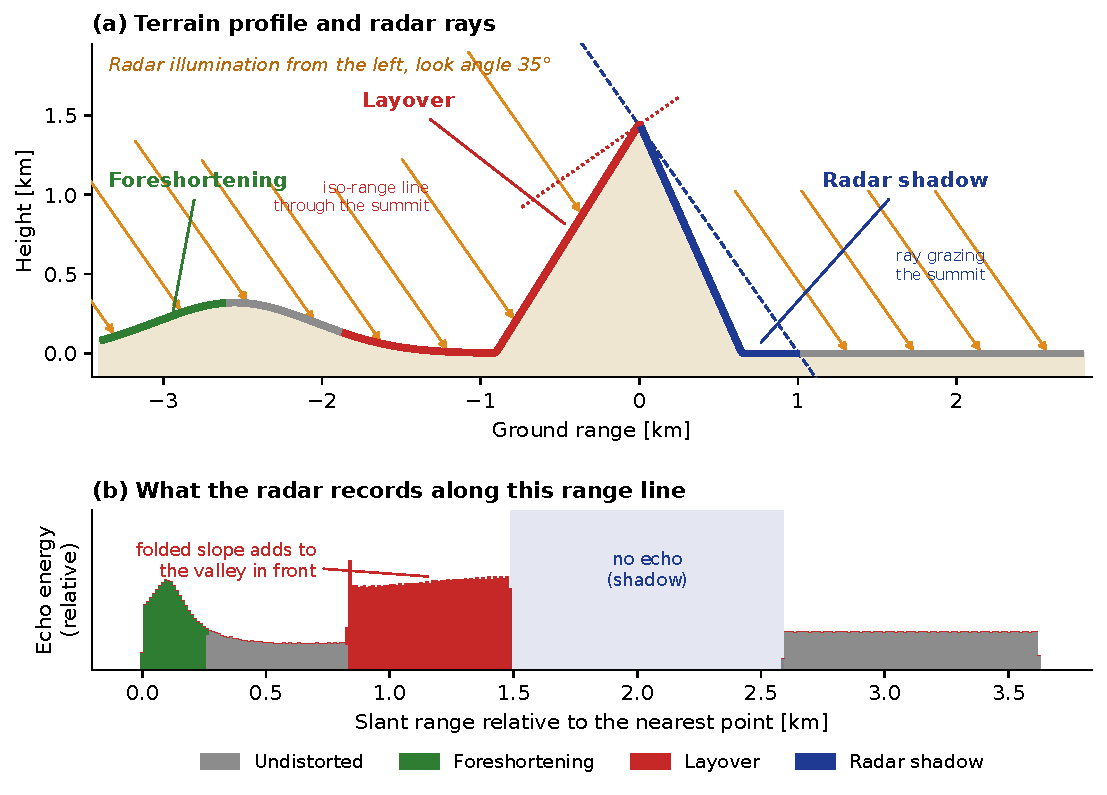
\includegraphics[width=\textwidth]{sar_distortions.pdf}
\caption[Geometric distortions of a side-looking SAR]{Geometric distortions of a side-looking SAR. (a) Terrain profile
illuminated from the left at a look angle of 35$^\circ$: the gentle slope facing the radar is foreshortened, the steep
fore-slope and the valley floor in front of it are in layover, and the back-slope and the terrain behind it lie in
radar shadow. (b) Echo energy recorded along this range line: the foreshortened slope is compressed and bright, the
folded fore-slope is added to the valley floor, and the shadow returns no echo.}
\label{fig:intro}
\end{figure}

Simulating the image that a SAR should record from a digital elevation model (DEM) is the classical way to understand,
predict and correct these effects. DEM-based simulations are used to geocode and terrain-correct SAR data
\cite{schreier1993,meier1993,small2011,low2007}, to generate layover and shadow masks \cite{kropatsch1990}, to estimate
the illuminated area for radiometric normalisation \cite{ulander1996,small2011,frey2013}, and to co-register images
precisely \cite{nitti2011}. Two recent developments make a fresh assessment timely. First, the Copernicus GLO-30 DEM
provides a consistent global elevation model at 1\,arcsec resolution \cite{copdem}. Second, Sentinel-1 Ground Range
Detected (GRD) products are distributed with a complete annotation of orbit state vectors, zero-Doppler timing,
slant-to-ground-range (SRGR) polynomials and radiometric calibration \cite{s1pd}, and are streamed as cloud-optimised
files without registration \cite{planetary}. Together, they allow a simulation to be computed in the exact geometry of a
product and compared with it pixel by pixel.

\section{Problem Statement}
Although DEM-based simulation is an established tool, it is usually embedded in large processing systems whose
internal assumptions are not visible to the user, and it is rarely assessed against real images beyond a visual
comparison. What is less well documented is how far such a DEM-only simulation goes in explaining a real C-band image of
high-relief terrain, which processing choices matter for its geometric and radiometric agreement, and where the
remaining disagreement comes from. A transparent simulator, verified component by component and assessed
quantitatively against real Sentinel-1 data, is required to answer these questions.

\section{Objectives}
The objectives of this work are:
\begin{enumerate}
\item to build a transparent SAR simulator from first principles and verify each of its components quantitatively,
from the impulse response of a point target to a real DEM;
\item to drive the simulator with the annotated geometry of real Sentinel-1 GRD products and assess its geometric
accuracy against the products' own geolocation;
\item to assess the radiometric agreement with the real images for several backscatter laws, for two viewing
geometries and for several processing choices;
\item to identify, with an independent land-cover map, which part of the image a DEM cannot explain.
\end{enumerate}

\section{Scope of the Work}
The study is limited to C-band Sentinel-1 IW GRD products in VV polarisation over one Alpine study site around
Innsbruck, Austria, observed from one ascending and one descending pass. The simulator is an incoherent, single-bounce
image-domain model driven by the Copernicus GLO-30 DEM; double bounce, volume scattering and multi-temporal effects are
outside its scope and are discussed as limitations. All data are open and all software is released with the report.

\section{Organisation of the Report}
The report is organised as follows. Chapter~\ref{ch:literature} reviews SAR image formation, the geometric and
radiometric effects of terrain, and existing SAR simulators. Chapter~\ref{ch:data} describes the study site and the
data. Chapter~\ref{ch:method} presents the raw-signal and image-domain simulators, the range-Doppler geocoding, the
treatment of shadow, layover and radiometry, the comparison strategy and the finalized design.
Chapter~\ref{ch:results} presents and discusses the results, including the limitations of the study.
Chapter~\ref{ch:software} describes the software that implements the work, and Chapter~\ref{ch:conclusions} draws the
conclusions and outlines future work.

\chapter{Literature Review}
\label{ch:literature}
This chapter summarises the principles of SAR image formation and the effects of terrain on SAR images that the
simulator has to reproduce, and reviews the existing approaches to SAR simulation and DEM-based geocoding.

\section{Range Resolution and Pulse Compression}
A SAR transmits a linear frequency-modulated pulse (chirp) $s(t)=\exp(j\pi K_r t^2)$ for $|t|<T_p/2$, of bandwidth
$B=K_rT_p$. A scatterer at slant range $R$ returns a copy of the pulse delayed by $2R/c$ and phase-shifted by
$-4\pi R/\lambda$. Correlating the echo with the transmitted replica (matched filtering) compresses the long pulse into a
sinc-shaped peak whose $-3$\,dB width defines the slant-range resolution
\begin{equation}
\rho_r = 0.886\,\frac{c}{2B}, \qquad \rho_g = \frac{\rho_r}{\sin\theta},
\end{equation}
where $\rho_g$ is the corresponding ground-range resolution at incidence angle $\theta$ \cite{cumming2005,curlander1991}.
The resolution therefore depends on the bandwidth and not on the pulse length, which can be chosen long enough to
deliver the required energy.

\section{Azimuth Resolution and the Synthetic Aperture}
Along the flight track (azimuth) a single pulse cannot separate targets, since the real antenna beam is several
kilometres wide on the ground. As the platform moves with speed $v$, the range to a target follows the hyperbola
$R(\eta)=\sqrt{R_0^2+v^2\eta^2}$, which produces a phase history $\exp(-j4\pi R(\eta)/\lambda)$ that is a chirp in
Doppler with a rate of $2v^2/(\lambda R_0)$. Matched filtering in azimuth over the synthetic aperture
$L_{sa}=\lambda R_0/L$, where $L$ is the antenna length, yields an azimuth resolution of about $L/2$, independent of
range \cite{moreira2013,curlander1991}. Several focusing algorithms exist; time-domain back-projection, in which the
range-compressed samples at the exact range of every image point are phase-corrected and summed over all pulses, is
the most direct and is exact for arbitrary scene geometry \cite{cumming2005}.

\section{Speckle}
A natural surface contains many elementary scatterers per resolution cell. Their coherent sum has a random phase, so
that the single-look intensity of a homogeneous surface is exponentially distributed with a standard deviation equal to
its mean \cite{goodman1976}. Averaging $L$ independent looks (multilooking) produces a Gamma distribution with a
relative variance of $1/L$, at the cost of spatial resolution \cite{oliver1998}. Speckle is therefore a property of the
measurement rather than of the surface, and comparisons between simulated and real images are made on multilooked
data.

\section{Geometric Distortions in Mountainous Terrain}
Because a SAR orders echoes by slant range, terrain height $h$ shifts a point towards the sensor by $h\cot\theta$ in
ground range, and the slope of the terrain controls how much ground falls into each range cell
\cite{leberl1990}. Three regimes follow (Fig.~\ref{fig:intro}). Slopes facing the radar with a slope smaller than the
look angle are compressed into fewer range cells and appear bright (foreshortening). If the slope exceeds the look
angle, the top of the slope is closer to the radar than its foot, so that the slope is imaged reversed and mixed with
the terrain in front of it (layover). Slopes facing away from the radar with a slope larger than the complement of the
look angle, together with all terrain hidden behind them, return no echo (radar shadow). Kropatsch and Strobl
\cite{kropatsch1990} showed how layover and shadow maps can be derived from a DEM, and Gelautz et al.
\cite{gelautz1998} analysed simulated and real SAR images of Alpine terrain, where these effects are pervasive.

\section{Radiometry and Backscatter Models}
The radar cross-section per unit ground area, $\sigma^0$, depends on the surface material, its roughness and moisture,
and on the local incidence angle $\theta_{loc}$ between the radar beam and the surface normal
\cite{ulaby1982,ulaby1989}. Simulators commonly reduce this dependence to a simple law of $\theta_{loc}$, such as the
cosine law, Lambert's law ($\cos^2\theta_{loc}$) or Muhleman's law \cite{muhleman1964}, whose validity for real
terrain remains an empirical question. In addition, the area of terrain that maps into one image pixel varies with the
topography. ESA calibrates GRD products to $\sigma^0$ referred to the ellipsoid pixel area, so that the brightness of a
pixel contains both effects; separating them is the purpose of radiometric slope correction and terrain flattening
\cite{ulander1996,small2011,frey2013}.

\section{SAR Simulators and DEM-Based Geocoding}
SAR simulators span a wide range of complexity. Raw-signal simulators generate the echo of every pulse and are used to
test focusing algorithms and system designs \cite{franceschetti1992}. Ray tracers model multiple bounces in urban
scenes and are used to interpret high-resolution images of buildings \cite{balz2009,auer2010}. Image-domain
simulators, finally, project each DEM facet directly into the image and form the basis of operational geocoding and
terrain correction \cite{schreier1993,meier1993,small2011,low2007}; they are also used for DEM-assisted co-registration
in interferometry \cite{nitti2011,bamler1998}. The absolute geolocation accuracy of Sentinel-1 products, which bounds
how well any simulation can be aligned with them without co-registration, has been verified with corner reflectors and
reaches a few metres when atmospheric delay and solid-earth tides are corrected \cite{schubert2015,gisinger2021}.

\section{Research Gap}
Existing studies either use DEM-based simulation as an internal step of geocoding and terrain-correction chains, or
analyse simulated images qualitatively. A transparent simulator that is verified from its physical principles upwards,
driven by the exact annotation of current Sentinel-1 products, and assessed quantitatively against real images for
several backscatter laws, viewing geometries, processing choices and land-cover classes is not readily available. This
work addresses this gap.

\chapter{Study Area and Data}
\label{ch:data}
\section{Study Site}
The study site (11.25--11.55$^\circ$\,E, 47.15--47.35$^\circ$\,N; approximately $23\times22$\,km$^2$) is centred on the city of Innsbruck in Tyrol, Austria (Fig.~\ref{fig:site}). The east--west oriented Inn valley, with a floor at about 580\,m above sea level, separates the steep south face of the Nordkette (up to 2300\,m) in the north from the Patscherkofel and the Stubai pre-Alps in the south; the Sill gorge (Wipptal) enters the valley from the south. Elevations within the site range from 552\,m to 2789\,m. The site therefore contains all regimes of geometric distortion and a strong land-cover contrast between the urbanised valley floor, extensive forests, alpine grassland and bare rock.

\begin{figure}[htbp]
\centering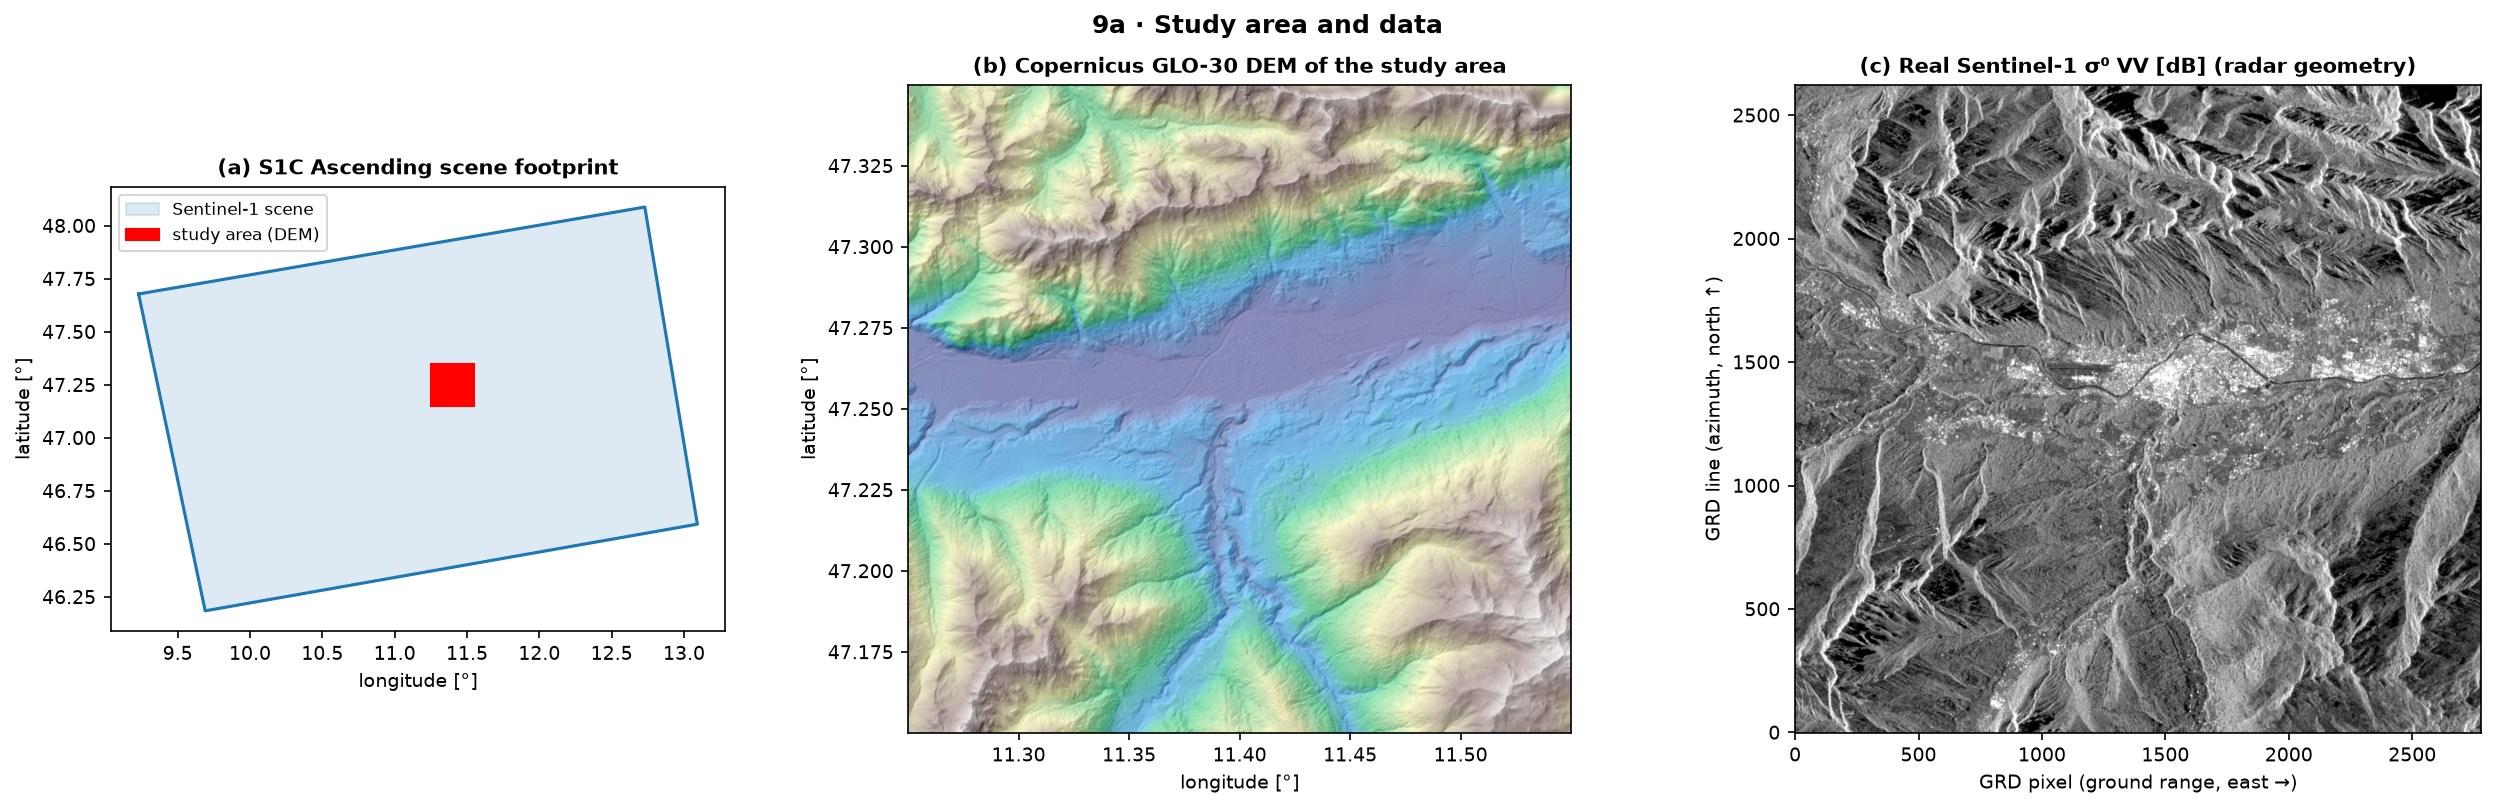
\includegraphics[width=\textwidth]{09a_study_area_data.png}
\caption[Study site and data]{Study site and data. (\textbf{a}) Footprint of the ascending Sentinel-1 scene and the study site (red). (\textbf{b}) Copernicus GLO-30 DEM of the study site. (\textbf{c}) Calibrated Sentinel-1 $\sigz$ (VV) of the study site in radar geometry.}
\label{fig:site}
\end{figure}

\section{Digital Elevation Model}
The Copernicus GLO-30 DEM~\cite{copdem} tile N47\,E011 was cropped to the study site, yielding $720\times1080$ samples at 1\,arcsec spacing (about 31\,m north--south and 21\,m east--west). GLO-30 heights refer to the EGM2008 geoid~\cite{pavlis2012}; they were converted to WGS84 ellipsoidal heights with the geoid undulation $N=\geoidN$\,m obtained from the EGM2008 model, as required by the orbit-based geocoding.

\section{Sentinel-1 Data}
Two Sentinel-1C Interferometric Wide-swath (IW) GRD high-resolution products in VV polarisation, one from an ascending and one from a descending pass, were selected as the most recent scenes in August--September 2025 that fully cover the site (Table~\ref{tab:s1}). The ascending pass looks east and the descending pass looks west, so that the two geometries illuminate opposite slopes. Only the window of each GRD image that covers the DEM (about $2600\times2780$ pixels of $10\times10$\,m) was read from the cloud-optimised file. For each product, the annotation provides the orbit state vectors (10\,s spacing), the zero-Doppler time of the first line and the azimuth time interval, 28 time-tagged SRGR polynomials, the geolocation grid (210 tie points) and the radiometric calibration look-up table~\cite{s1pd}.

\begin{table}[htbp]
\caption[Sentinel-1 data used in this study]{Sentinel-1 data used in this study. Incidence angle at mid-swath; window size in GRD pixels.}
\label{tab:s1}
\centering\small
\begin{tabularx}{\textwidth}{lXX}
\toprule
 & \textbf{Ascending} & \textbf{Descending}\\\midrule
Platform, mode, polarisation & \platAsc, IW GRDH, VV & \platDesc, IW GRDH, VV\\
Acquisition start (UTC) & \dateAsc, 17:06:22 & \dateDesc, 05:17:54\\
Absolute orbit & 4313 & 4291\\
Look direction & east & west\\
Incidence angle (mid-swath) & \incAsc$^\circ$ & \incDesc$^\circ$\\
Pixel spacing (range $\times$ azimuth) & $10\times10$\,m & $10\times10$\,m\\
Window covering the DEM & $2622\times2780$ & $2600\times2772$\\
\bottomrule
\end{tabularx}
\end{table}

\section{Land Cover}
The ESA WorldCover 2021 map at 10\,m resolution~\cite{worldcover} was sampled at the DEM grid by nearest-neighbour interpolation. Within the analysed area, tree cover represents 55\,\% of the pixels, grassland 26\,\%, built-up areas 7\,\%, bare or sparsely vegetated land 6\,\% and cropland 4\,\%; water, snow and ice, and moss and lichen together represent about 2\,\%. All data sets were accessed through the Microsoft Planetary Computer~\cite{planetary}.

\chapter{Methodology}
\label{ch:method}
The simulator was developed incrementally, from a single point target to a full Sentinel-1 scene. Each stage had to pass a quantitative test before the next stage was built, and the tests that failed determined the design decisions of the final processing chain (Fig.~\ref{fig:design}). The final data flow is summarised in Fig.~\ref{fig:dataflow}.

\section{Raw-Signal Simulator}
\label{sec:raw}
To verify the physics of the simulation, a raw-signal simulator was implemented for a sensor with Sentinel-1-like parameters (wavelength $\lambda=5.55$\,cm, chirp bandwidth $B=50$\,MHz, pulse length $T_p=10\,\mu$s, sampling rate 60\,MHz, antenna length $L=12.3$\,m, pulse repetition frequency 1700\,Hz) flying a straight track at 693\,km altitude with a look angle of 35$^\circ$ over a flat Earth. The transmitted pulse is the linear frequency-modulated chirp
\begin{equation}
s(t)=\exp\!\left(j\pi K_r t^2\right),\qquad |t|<T_p/2,\qquad K_r=B/T_p .
\end{equation}
For a set of point scatterers with complex reflectivity $a_i$ at positions $\mathbf{P}_i$, the echo received at slow time $\eta$ is
\begin{equation}
e(t,\eta)=\sum_i a_i\,G\!\left(\vartheta_i(\eta)\right)\,s\!\left(t-\frac{2R_i(\eta)}{c}\right)\exp\!\left(-j\frac{4\pi R_i(\eta)}{\lambda}\right),
\label{eq:raw}
\end{equation}
where $R_i(\eta)$ is the range from the sensor to scatterer $i$ and $G$ is the two-way azimuth antenna pattern $\mathrm{sinc}^2(L\vartheta/\lambda)$ of the squint angle $\vartheta$. Equation~(\ref{eq:raw}) is evaluated efficiently by placing a band-limited impulse at the exact fractional delay of each scatterer and convolving with the chirp in the frequency domain. Range compression is performed by matched filtering with the chirp replica, and azimuth compression by time-domain back-projection,
\begin{equation}
I(\mathbf{x})=\sum_{\eta} s_{rc}\!\left(\frac{2R(\mathbf{x},\eta)}{c},\eta\right)\exp\!\left(j\frac{4\pi R(\mathbf{x},\eta)}{\lambda}\right),
\end{equation}
which is exact for arbitrary scene geometry and therefore also displaces elevated points towards the sensor when the image is formed on a flat reference plane. The simulator was verified on a single point target, on lines of targets, on three targets observed along the synthetic aperture, on fields of randomly distributed scatterers (speckle), on a sinusoidal surface and on a $480\times480$\,m patch of the Copernicus DEM (Section~\ref{sec:res-verif}).

\section{Image-Domain Simulator}
Because generating raw data for millions of scatterers is impractical, scene-scale simulations use an image-domain simulator: every DEM facet is projected directly to its zero-Doppler position (azimuth time, slant range), its backscattered power is accumulated in the image grid and, for comparison with focused raw-signal simulations, blurred with the impulse response measured in Section~\ref{sec:res-verif}. The equivalence of the two approaches was verified on the sinusoidal surface and on the DEM patch.

\section{Range-Doppler Geocoding in Sentinel-1 GRD Geometry}
For the real scenes, the orbit state vectors within $\pm90$\,s of the scene are fitted with a polynomial of degree 7 per ECEF coordinate; its derivative reproduces the annotated velocities to 0.1\,mm/s. For a ground point $\mathbf{X}$, the zero-Doppler azimuth time $t$ solves
\begin{equation}
f(t)=\left(\mathbf{X}-\mathbf{S}(t)\right)\cdot\mathbf{V}(t)=0,
\label{eq:zd}
\end{equation}
where $\mathbf{S}$ and $\mathbf{V}$ are the sensor position and velocity. Equation~(\ref{eq:zd}) is solved by Newton iteration with $f'(t)=-|\mathbf{V}|^2+(\mathbf{X}-\mathbf{S})\cdot\mathbf{A}$; eight iterations reach machine precision. The GRD line is $t/\Delta t_{az}$, with $t$ measured from the first image line. The slant range $R=|\mathbf{X}-\mathbf{S}(t)|$ is converted to ground range with the annotated SRGR polynomial
\begin{equation}
g(R)=\sum_{k=0}^{8}c_k\,(R-R_0)^k ,
\end{equation}
and the GRD pixel is $g/\Delta_{gr}$. The annotation lists one polynomial set per second of azimuth time. Interpolating linearly between consecutive sets, an apparently natural choice, produced range errors of up to 3.3 pixels with respect to the geolocation grid of the product, because consecutive sets differ by up to 19 pixels. Applying each set from its time tag until the next one (``valid-from'' rule) removes this error (Section~\ref{sec:res-geo}).

\section{DEM Facets, Local Incidence Angle, Shadow and Layover}
The ellipsoidal DEM is oversampled three times by bilinear interpolation (about $10\times7$\,m facets, smaller than a GRD pixel) and converted to ECEF coordinates. Facet normals $\hat{\mathbf{n}}$ and true facet areas $A$ follow from the cross product of the grid tangent vectors, and the local incidence angle from $\cos\theta_{loc}=-\hat{\mathbf{u}}\cdot\hat{\mathbf{n}}$, with $\hat{\mathbf{u}}$ the unit look vector. To detect shadow and layover, facets are sorted along each azimuth line by their ground position $\psi$ (geocentric angle from the sensor). A facet is in shadow if a facet closer to the ground track is seen under a larger off-nadir angle $\alpha$, and in layover if a closer facet has a larger slant range or a farther facet a smaller one:
\begin{equation}
\mathrm{shadow}:\ \alpha<\max_{\psi'<\psi}\alpha',\qquad \mathrm{layover}:\ R<\max_{\psi'<\psi}R' \ \ \lor\ \ R>\min_{\psi'>\psi}R' .
\end{equation}
The grouped running extrema are computed in one vectorised pass. For the 7.0 million facets of a scene, the geometry is computed in blocks of DEM rows and stored in single precision (about 34 bytes per facet), which keeps the memory footprint at about 240\,MB.

\section{Radiometric Model}
Each illuminated facet contributes $\sigz(\theta_{loc})\,A$ to the four GRD pixels surrounding its fractional (line, pixel) position by bilinear splatting, and the sum is divided by the ellipsoid pixel area $\Delta_{az}\Delta_{gr}$. The simulated image is therefore in the same unit as ESA-calibrated $\sigz$, which refers to the ellipsoid~\cite{small2011}. Five backscatter laws were compared: a constant law, which retains only the illuminated-area term; the cosine law $\sigz\propto\cos\theta_{loc}$; Lambert's law $\sigz\propto\cos^2\theta_{loc}$~\cite{ulaby1982}; Muhleman's law~\cite{muhleman1964},
\begin{equation}
\sigz(\theta_{loc})=0.0133\,\frac{\cos\theta_{loc}}{\left(\sin\theta_{loc}+0.1\cos\theta_{loc}\right)^3},
\end{equation}
and a law $\sigz=k\cos^{n}\theta_{loc}$ fitted to the real image. The fit is a least-squares regression of the median real $\sigz$ (in dB) in 2$^\circ$ bins of $\theta_{loc}$ between 5$^\circ$ and 80$^\circ$, excluding layover and shadow, on $10\log_{10}\cos\theta_{loc}$.

\section{Comparison with Sentinel-1}
Real digital numbers were calibrated to $\sigz=\mathrm{DN}^2/A_\sigma^2$ with the bilinearly interpolated calibration table; thermal noise was not removed. Real and simulated images were multilooked with a $5\times5$ boxcar ($50\times50$\,m) and converted to dB. The simulation was co-registered to the real image by sub-pixel cross-correlation within the largest fully valid interior box of the footprint, and its absolute level was calibrated by a single constant, the median difference between real and simulated $\sigz$ in dB. Agreement is reported as the Pearson correlation $r$ and the Spearman correlation $\rho$ over all valid pixels, the structural similarity index (SSIM)~\cite{wang2004} within the interior box, and the root mean square difference (RMSE) after level calibration. For analyses in map geometry, the real image is back-geocoded to the DEM grid using the facet positions.

\section{Experimental Design}
The following experiments were carried out (Fig.~\ref{fig:dataflow}):
\begin{itemize}
\item E1, backscatter laws: the five laws are applied to the same ascending geometry.
\item E2, second viewing geometry: the law fitted on the ascending scene is applied, unchanged, to the descending scene, which acts as an independent validation.
\item E3, geometric validation: the geocoding is compared with the geolocation grid of both products, and the real $\sigz$ is analysed inside the predicted shadow, layover and foreshortening classes.
\item E4, sensitivity: the simulation is repeated without geoid correction, without DEM oversampling and with a 90\,m DEM obtained by $3\times3$ aggregation of GLO-30.
\item E5, land cover: the residual (real minus simulated) is analysed per WorldCover class in map geometry.
\end{itemize}

\begin{figure}[htbp]
\centering
\resizebox{\textwidth}{!}{% Data flow of the simulator (shared style with the A3 poster)
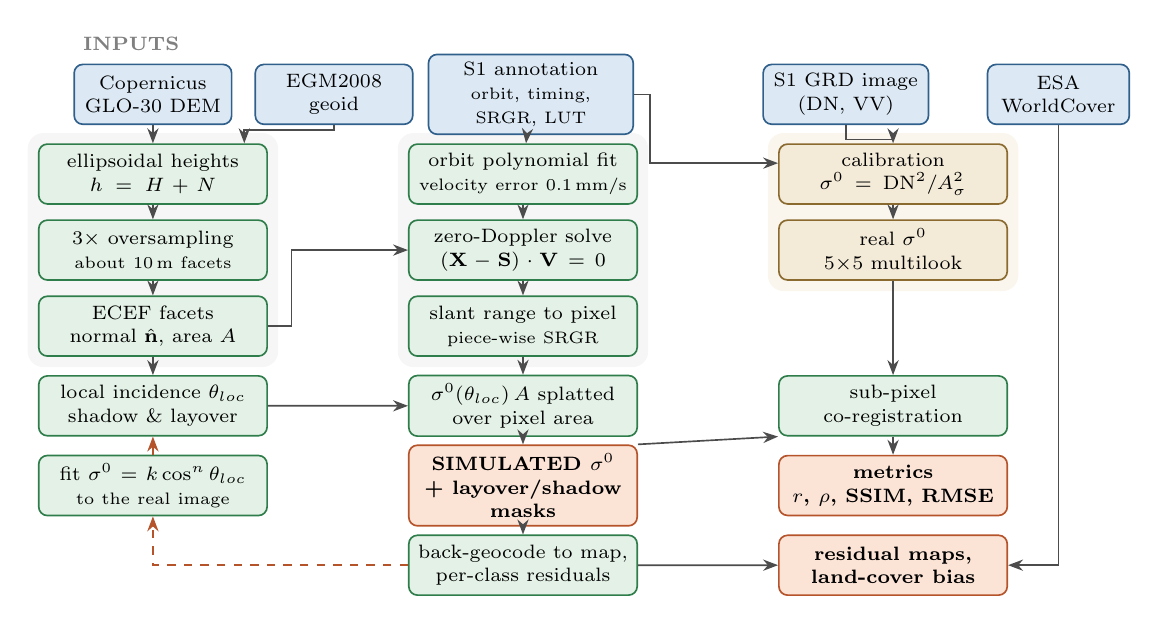
\begin{tikzpicture}[yscale=0.92,
  font=\fontsize{7.4}{8.6}\selectfont, >={Stealth[length=1.9mm]},
  base/.style={draw, rounded corners=1.1mm, align=center, minimum height=7.6mm, inner sep=1mm, line width=0.6pt},
  inp/.style={base, fill=inC, draw=inD, text width=19mm},
  pro/.style={base, fill=prC, draw=prD, text width=27mm},
  rea/.style={base, fill=reC, draw=reD, text width=27mm},
  prod/.style={base, fill=ouC, draw=ouD, text width=27mm, font=\fontsize{7.4}{8.6}\selectfont\bfseries},
  ar/.style={->, line width=0.6pt, draw=black!70},
  fb/.style={->, line width=0.75pt, draw=ouD, dashed}]
\def\xA{0mm} \def\xB{47mm} \def\xC{94mm}
\node[inp, text width=18mm] (dem) at (\xA,0) {Copernicus\\GLO-30 DEM};
\node[inp, text width=18mm] (geo) at (23mm,0) {EGM2008\\geoid};
\node[inp, text width=24mm] (ann) at (\xB+1mm,0) {S1 annotation\\{\fontsize{6.4}{7.2}\selectfont orbit, timing, SRGR, LUT}};
\node[inp, text width=19mm] (grd) at (\xC-6mm,0) {S1 GRD image\\(DN, VV)};
\node[inp, text width=16mm] (wc) at (\xC+21mm,0) {ESA\\WorldCover};
\node[pro] (hgt)  at (\xA,-11mm) {ellipsoidal heights\\$h=H+N$};
\node[pro] (orb)  at (\xB,-11mm) {orbit polynomial fit\\{\fontsize{6.4}{7.2}\selectfont velocity error 0.1\,mm/s}};
\node[rea] (cal)  at (\xC,-11mm) {calibration\\$\sigma^0=\mathrm{DN}^2/A_\sigma^2$};
\node[pro] (ovs)  at (\xA,-21.5mm) {3$\times$ oversampling\\{\fontsize{6.4}{7.2}\selectfont about 10\,m facets}};
\node[pro] (zd)   at (\xB,-21.5mm) {zero-Doppler solve\\$(\mathbf X-\mathbf S)\cdot\mathbf V=0$};
\node[rea] (rml)  at (\xC,-21.5mm) {real $\sigma^0$\\5$\times$5 multilook};
\node[pro] (ecef) at (\xA,-32mm) {ECEF facets\\normal $\hat{\mathbf n}$, area $A$};
\node[pro] (srgr) at (\xB,-32mm) {slant range to pixel\\{\fontsize{6.4}{7.2}\selectfont piece-wise SRGR}};
\node[pro] (inc)  at (\xA,-43mm) {local incidence $\theta_{loc}$\\shadow \& layover};
\node[pro] (spl)  at (\xB,-43mm) {$\sigma^0(\theta_{loc})\,A$ splatted\\over pixel area};
\node[pro] (reg)  at (\xC,-43mm) {sub-pixel\\co-registration};
\node[pro] (fit)  at (\xA,-54mm) {fit $\sigma^0=k\cos^n\theta_{loc}$\\{\fontsize{6.4}{7.2}\selectfont to the real image}};
\node[prod] (sim) at (\xB,-54mm) {SIMULATED $\sigma^0$\\+ layover/shadow masks};
\node[prod] (met) at (\xC,-54mm) {metrics\\$r$, $\rho$, SSIM, RMSE};
\node[pro]  (map) at (\xB,-65mm) {back-geocode to map,\\per-class residuals};
\node[prod] (res) at (\xC,-65mm) {residual maps,\\land-cover bias};
\draw[ar] (dem) -- (hgt);
\draw[ar] (geo.south) |- ($(hgt.north east)+(-3mm,1.8mm)$) -- ++(0,-1.8mm);
\draw[ar] (hgt) -- (ovs);
\draw[ar] (ovs) -- (ecef);
\draw[ar] (ann) -- (orb);
\draw[ar] (orb) -- (zd);
\draw[ar] (zd) -- (srgr);
\draw[ar] (ecef.east) -- ++(3mm,0) |- (zd.west);
\draw[ar] (ecef) -- (inc);
\draw[ar] (srgr) -- (spl);
\draw[ar] (inc) -- (spl);
\draw[ar] (spl) -- (sim);
\draw[ar] (grd.south) -- ++(0,-2mm) -| (cal.north);
\draw[ar] (ann.east) -- ++(2mm,0) |- ($(cal.west)+(0,1.5mm)$);
\draw[ar] (cal) -- (rml);
\draw[ar] (rml) -- (reg);
\draw[ar] (sim.north east) -- (reg.south west);
\draw[ar] (reg) -- (met);
\draw[ar] (sim) -- (map);
\draw[ar] (map) -- (res);
\draw[ar] (wc.south) |- (res.east);
\draw[fb] (map.west) -| (fit.south);
\draw[fb] (fit.north) -- (inc.south);
\node[font=\fontsize{7}{8}\selectfont\bfseries\color{black!50}, anchor=south west] at ($(dem.north west)+(0,0.5mm)$) {INPUTS};
\begin{scope}[on background layer]
  \node[fill=black!3.5, rounded corners=2mm, fit=(hgt)(ovs)(ecef), inner sep=1.3mm] {};
  \node[fill=black!3.5, rounded corners=2mm, fit=(orb)(zd)(srgr), inner sep=1.3mm] {};
  \node[fill=reC!45, rounded corners=2mm, fit=(cal)(rml), inner sep=1.3mm] {};
\end{scope}
\end{tikzpicture}
}
\caption[Data flow of the simulator]{Data flow of the simulator. Blue: inputs; green: simulation; beige: real-image path; orange: products. The dashed loop fits the backscatter law to the real image and feeds it back into the simulation.}
\label{fig:dataflow}
\vspace{8mm}
\resizebox{\textwidth}{!}{% Design evolution of the simulator (shared style with the A3 poster)
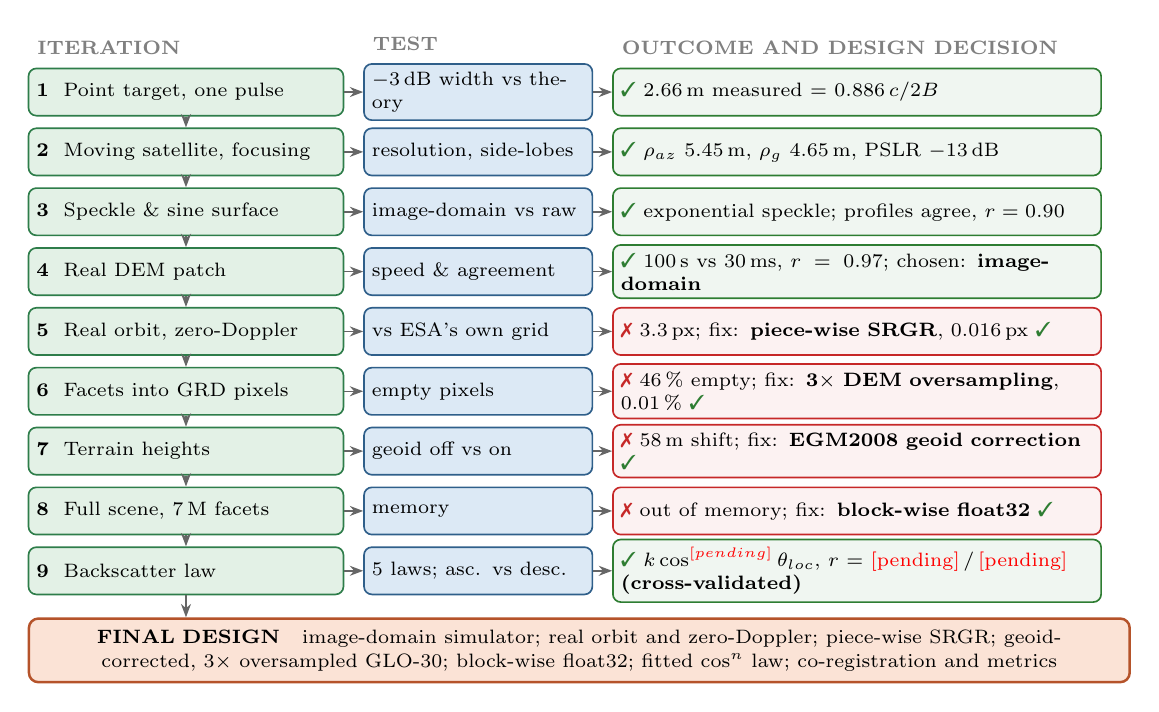
\begin{tikzpicture}[font=\fontsize{7.3}{8.4}\selectfont, >={Stealth[length=1.7mm]},
  st/.style={draw=prD, fill=prC, rounded corners=1mm, line width=0.6pt, text width=38mm, minimum height=6mm, align=left, inner sep=1mm},
  te/.style={draw=inD, fill=inC, rounded corners=1mm, line width=0.6pt, text width=27mm, minimum height=6mm, align=left, inner sep=1mm},
  okb/.style={draw=okC, fill=okC!7, rounded corners=1mm, line width=0.6pt, text width=60mm, minimum height=6mm, align=left, inner sep=1mm},
  nob/.style={draw=noC, fill=noC!6, rounded corners=1mm, line width=0.6pt, text width=60mm, minimum height=6mm, align=left, inner sep=1mm},
  ar/.style={->, line width=0.55pt, draw=black!60}]
\def\dy{7.6mm}
\foreach \i/\stage/\test/\res/\kind in {
  1/{\textbf{1}\ \ Point target, one pulse}/{$-3$\,dB width vs theory}/{\ok\ 2.66\,m measured = $0.886\,c/2B$}/okb,
  2/{\textbf{2}\ \ Moving satellite, focusing}/{resolution, side-lobes}/{\ok\ $\rho_{az}$ 5.45\,m, $\rho_g$ 4.65\,m, PSLR $-13$\,dB}/okb,
  3/{\textbf{3}\ \ Speckle \& sine surface}/{image-domain vs raw}/{\ok\ exponential speckle; profiles agree, $r=0.90$}/okb,
  4/{\textbf{4}\ \ Real DEM patch}/{speed \& agreement}/{\ok\ 100\,s vs 30\,ms, $r=0.97$; chosen: \textbf{image-domain}}/okb,
  5/{\textbf{5}\ \ Real orbit, zero-Doppler}/{vs ESA's own grid}/{\no\ 3.3\,px; fix: \textbf{piece-wise SRGR}, 0.016\,px \ok}/nob,
  6/{\textbf{6}\ \ Facets into GRD pixels}/{empty pixels}/{\no\ 46\,\% empty; fix: \textbf{3$\times$ DEM oversampling}, 0.01\,\% \ok}/nob,
  7/{\textbf{7}\ \ Terrain heights}/{geoid off vs on}/{\no\ 58\,m shift; fix: \textbf{EGM2008 geoid correction} \ok}/nob,
  8/{\textbf{8}\ \ Full scene, 7\,M facets}/{memory}/{\no\ out of memory; fix: \textbf{block-wise float32} \ok}/nob,
  9/{\textbf{9}\ \ Backscatter law}/{5 laws; asc. vs desc.}/{\ok\ $k\cos^{\nFit}\theta_{loc}$, $r$ = \rAsc\,/\,\rDesc\ \textbf{(cross-validated)}}/okb}{
  \node[st] (s\i) at (0,-\i*\dy) {\stage};
  \node[te, right=2.4mm of s\i] (t\i) {\test};
  \node[\kind, right=2.4mm of t\i] (r\i) {\res};
  \draw[ar] (s\i) -- (t\i);
  \draw[ar] (t\i) -- (r\i);
}
\foreach \i [count=\j from 2] in {1,...,8} { \draw[ar] (s\i) -- (s\j); }
\node[draw=ouD, fill=ouC, line width=0.9pt, rounded corners=1.2mm, align=center, inner sep=1.4mm,
      anchor=north west, font=\fontsize{7.5}{8.8}\selectfont, text width=137mm] (fin) at ($(s9.south west)+(0,-2.8mm)$)
  {\textbf{FINAL DESIGN}\quad image-domain simulator; real orbit and zero-Doppler; piece-wise SRGR; geoid-corrected, 3$\times$ oversampled GLO-30; block-wise float32; fitted $\cos^{n}$ law; co-registration and metrics};
\draw[ar] (s9) -- (s9|-fin.north);
\node[font=\fontsize{7}{8}\selectfont\bfseries\color{black!50}, anchor=south west] at ($(s1.north west)+(0,0.4mm)$) {ITERATION};
\node[font=\fontsize{7}{8}\selectfont\bfseries\color{black!50}, anchor=south west] at ($(t1.north west)+(0,0.4mm)$) {TEST};
\node[font=\fontsize{7}{8}\selectfont\bfseries\color{black!50}, anchor=south west] at ($(r1.north west)+(0,0.4mm)$) {OUTCOME AND DESIGN DECISION};
\end{tikzpicture}
}
\caption[Design evolution of the simulator]{Design evolution of the simulator. Each iteration had to pass the listed test before the next was built. Green: test passed; red: test failed, and the fix that became part of the final design.}
\label{fig:design}
\end{figure}

\section{Finalized Design}
\label{sec:final-design}
The final processing chain is the result of nine development iterations, summarised in Fig.~\ref{fig:design}. The
verification of the raw-signal simulator on a point target, on the synthetic aperture and on distributed and periodic
surfaces (iterations 1 to 3), and its comparison with the image-domain simulator on a real DEM patch (iteration 4), led
to the adoption of the image-domain simulator for scene-scale simulations. The four iterations that failed their test
fixed the remaining design decisions: the slant-to-ground-range polynomials are applied piece-wise rather than
interpolated (iteration 5), the DEM is oversampled three times so that every GRD pixel receives facets (iteration 6),
terrain heights are converted to ellipsoidal heights with the EGM2008 geoid (iteration 7), and the facet geometry is
computed block-wise in single precision so that a full scene fits in memory (iteration 8). The backscatter law,
finally, is fitted to the real image and cross-validated on the second viewing geometry (iteration 9). The resulting
data flow is the one shown in Fig.~\ref{fig:dataflow}.

\chapter{Results and Discussion}
\label{ch:results}
\section{Verification of the Simulators}
\label{sec:res-verif}
The single-pulse simulation of a point target (Fig.~\ref{fig:point}) reproduces the textbook behaviour of pulse compression: the 10\,$\mu$s echo, about 1.5\,km long in slant range, is compressed into a sinc-shaped peak with a measured $-3$\,dB width of 2.66\,m, equal to the theoretical value $0.886\,c/2B$. Five targets distributed over 160\,m of ground range produce overlapping echoes that are separated after compression, and two targets remain resolved down to a separation of about one ground-range resolution cell of 5.2\,m (Fig.~\ref{fig:line}).

\begin{figure}[htbp]
\centering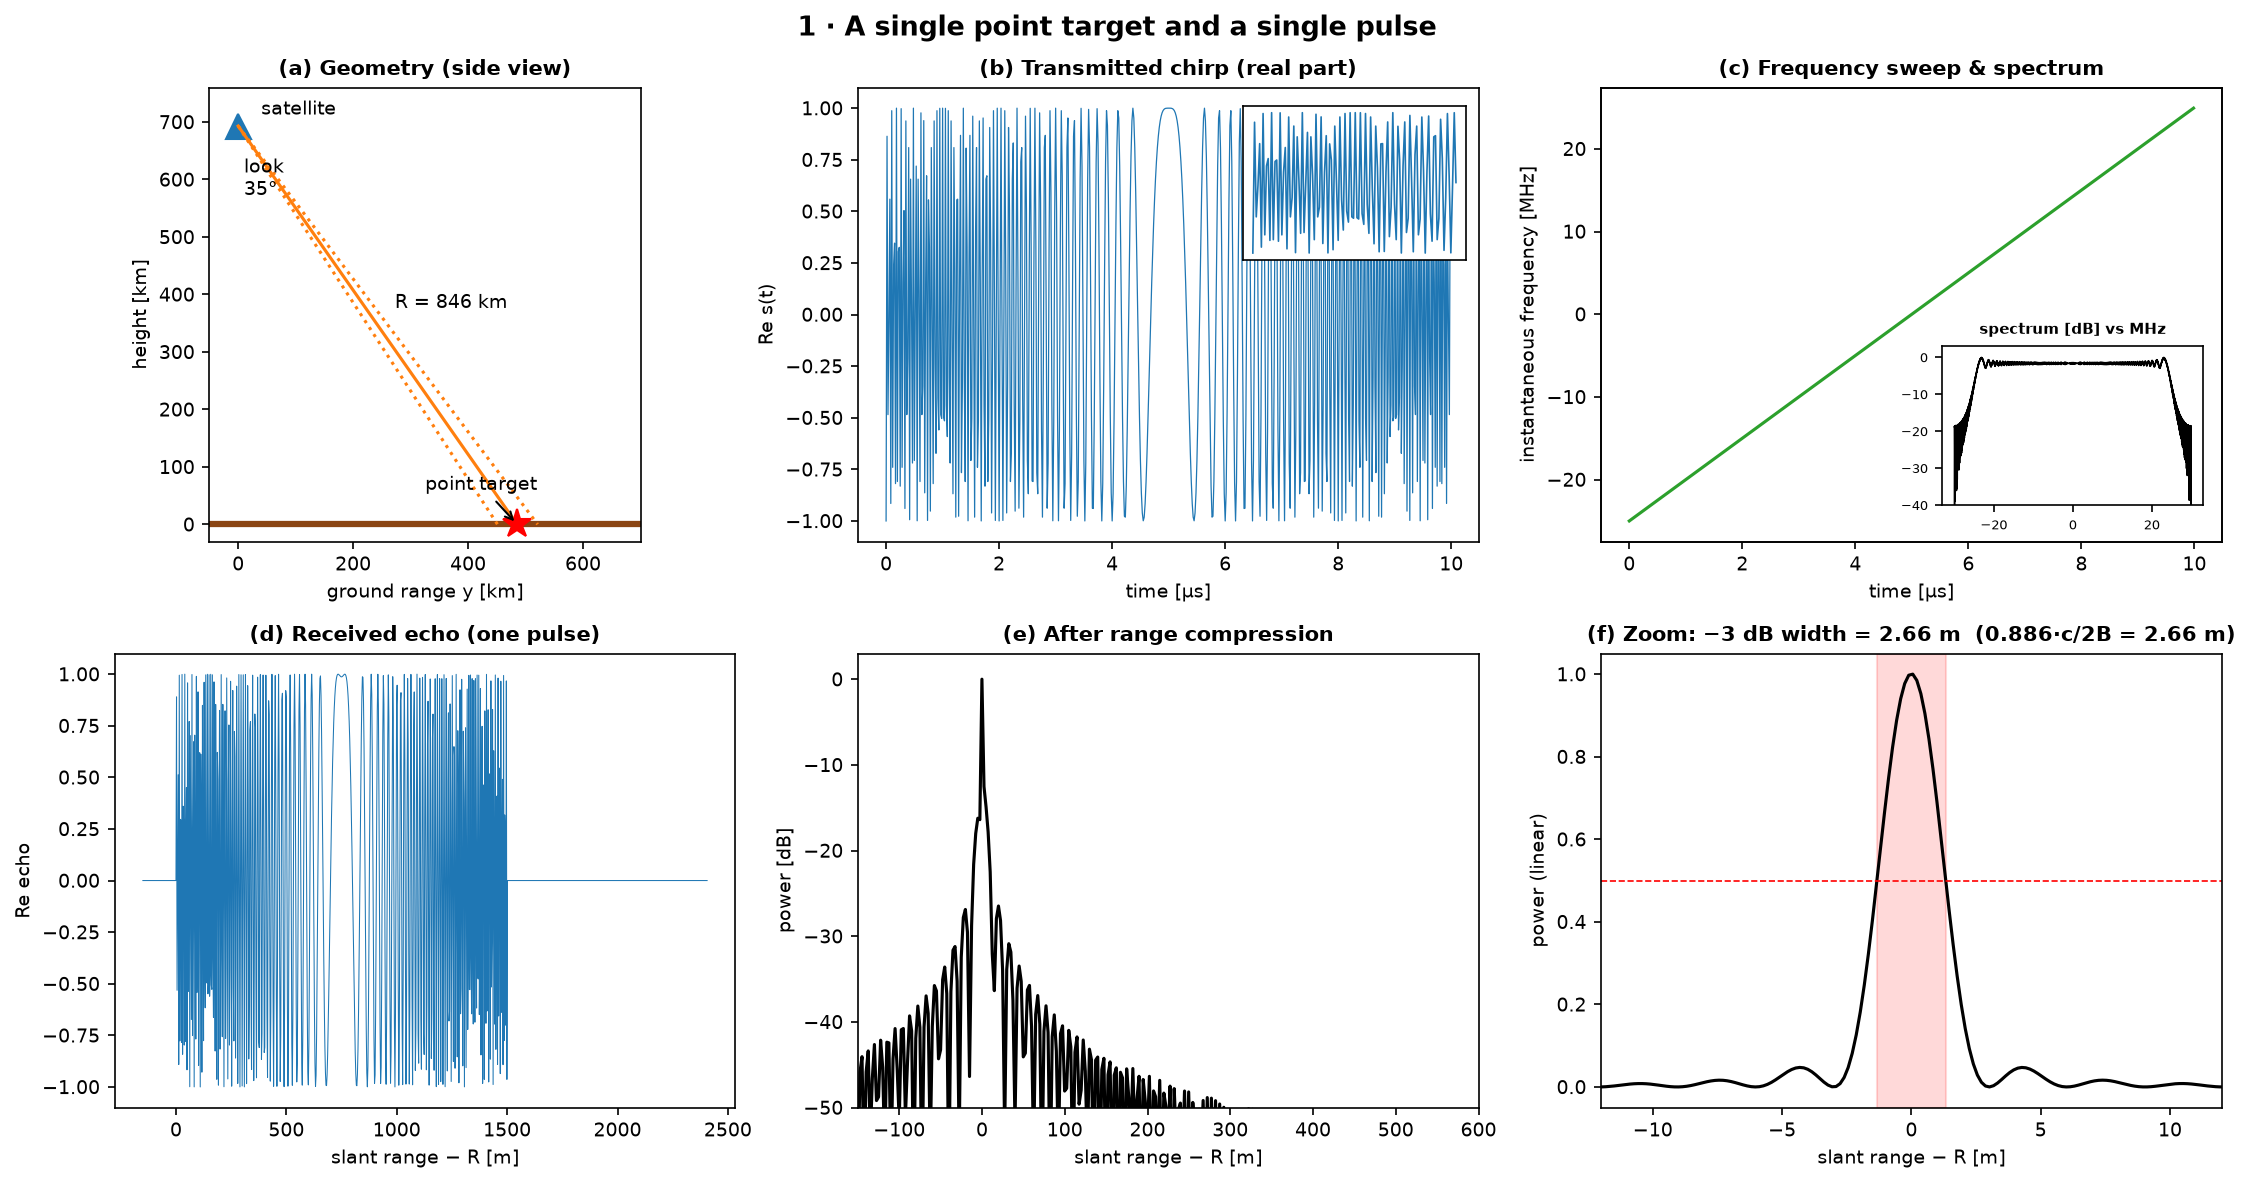
\includegraphics[width=\textwidth]{01_point_single_pulse.png}
\caption[A single point target illuminated by one pulse]{A single point target illuminated by one pulse: (\textbf{a}) geometry; (\textbf{b}) transmitted chirp; (\textbf{c}) frequency sweep and spectrum; (\textbf{d}) received echo; (\textbf{e}) range-compressed signal; (\textbf{f}) $-3$\,dB width of the compressed peak.}
\label{fig:point}
\end{figure}
\begin{figure}[htbp]
\centering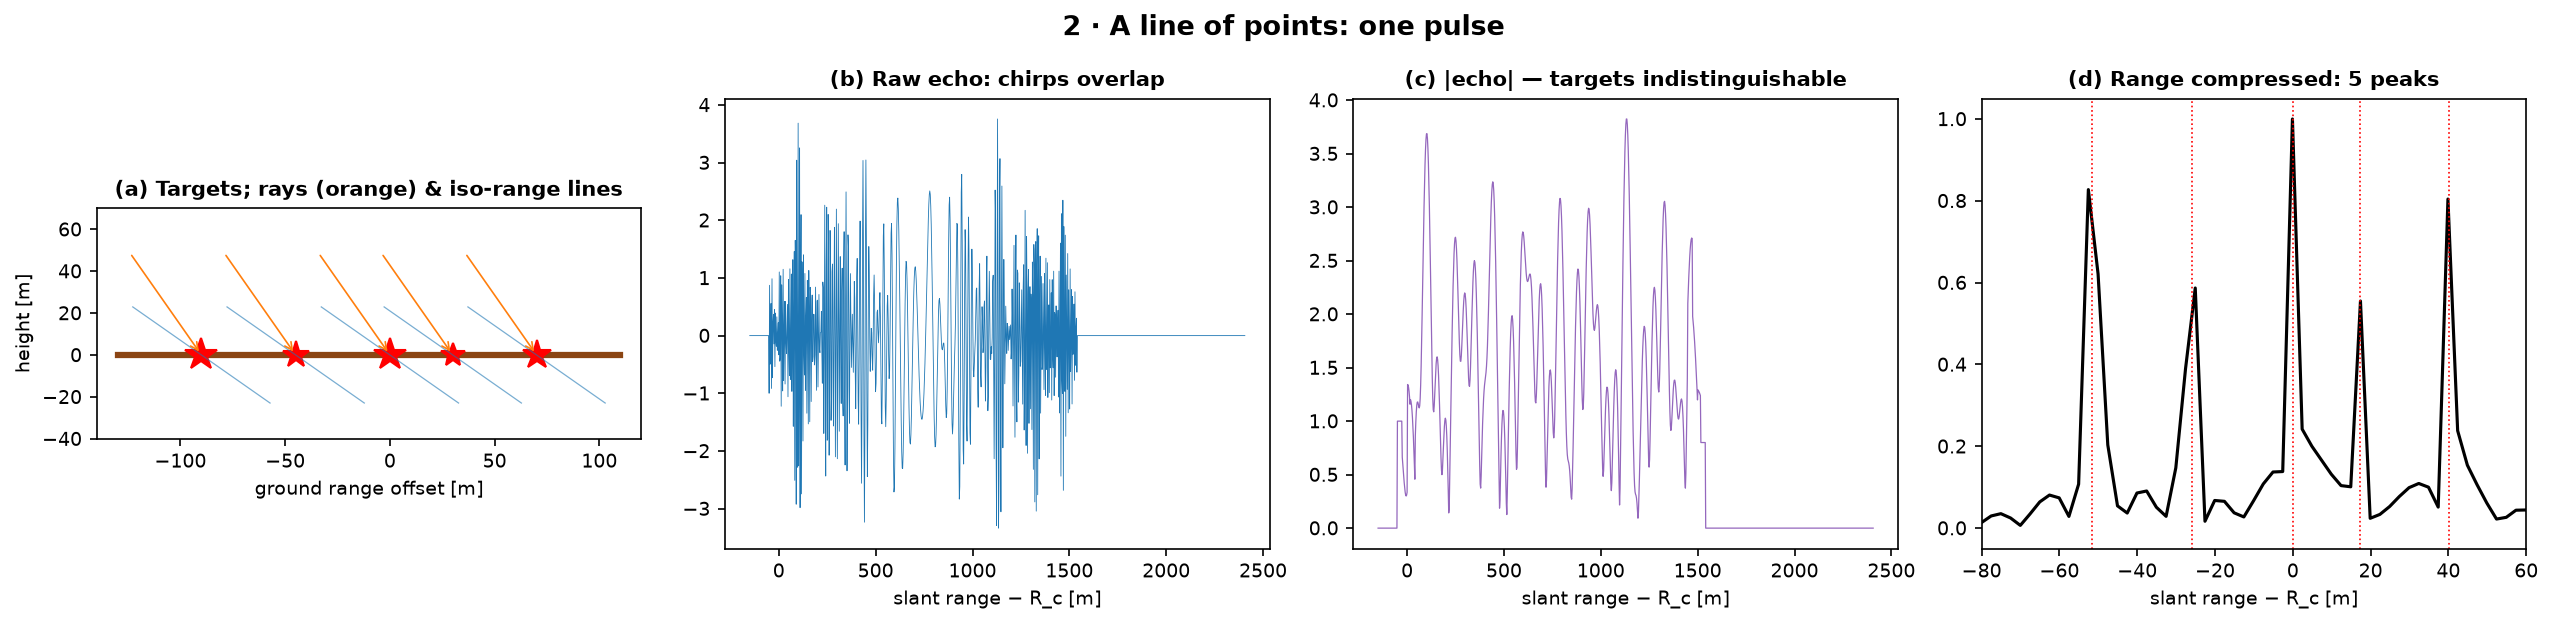
\includegraphics[width=\textwidth]{02_line_of_points.png}\\[2pt]
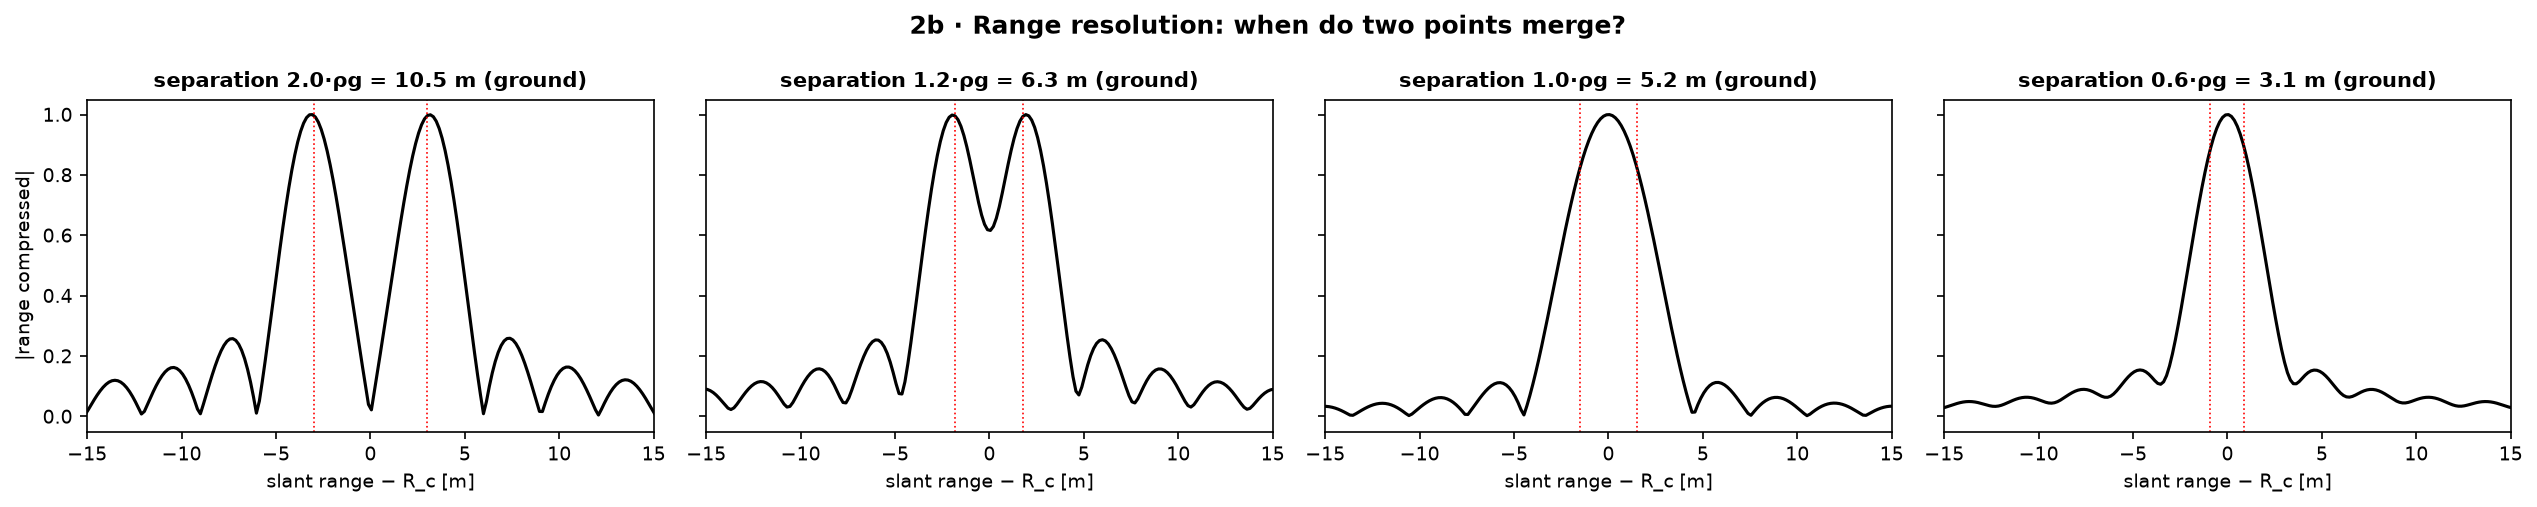
\includegraphics[width=\textwidth]{02b_range_resolution.png}
\caption[A line of point targets and the range resolution]{A line of point targets and the range resolution. Top: five targets on a line, their overlapping echoes and the compressed range profile. Bottom: two equal targets at decreasing separation, expressed in multiples of the ground-range resolution $\rho_g$.}
\label{fig:line}
\end{figure}

Along the synthetic aperture, each target follows a hyperbolic range history and a linear Doppler history (Fig.~\ref{fig:moving}). For the spaceborne geometry the range migration over the processed aperture of 4.6\,km is only 3.2\,m, about one range resolution cell, so that the range-compressed azimuth chirps are nearly straight. Back-projection focuses the three targets at their true positions with measured resolutions of 5.45\,m in azimuth and 4.65\,m in ground range and peak side-lobe ratios of $-23.6$\,dB and $-13.3$\,dB, respectively (Fig.~\ref{fig:irf}); the theoretical values are $L/2=6.15$\,m and $0.886\,\rho_r/\sin\theta=4.63$\,m. The lower azimuth side-lobes result from the antenna pattern, which acts as a taper.

\begin{figure}[htbp]
\centering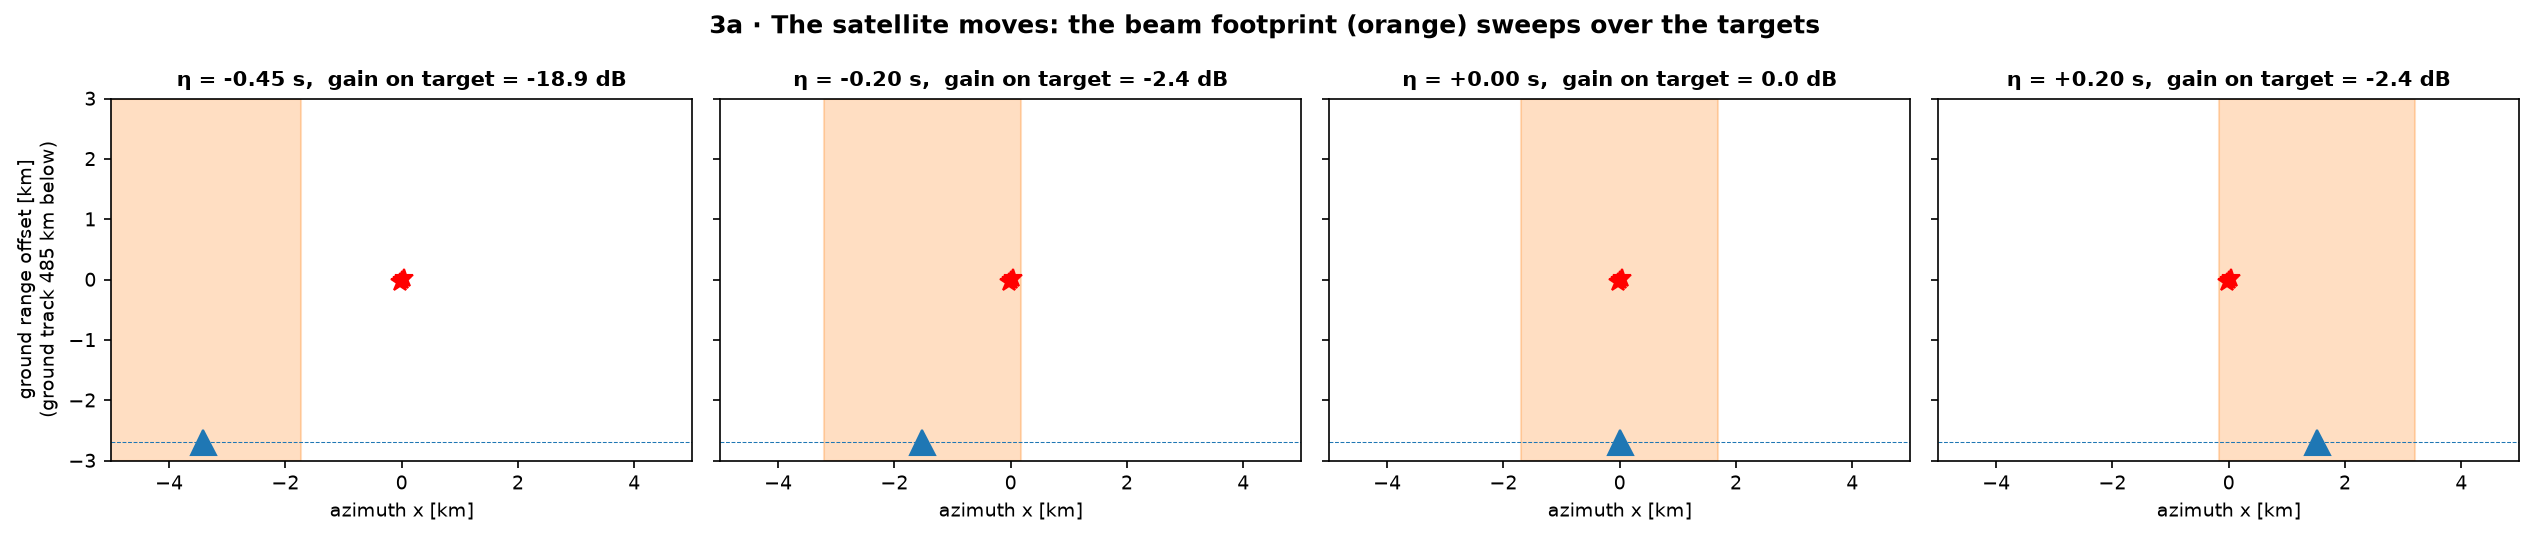
\includegraphics[width=\textwidth]{03a_moving_satellite_snapshots.png}\\[2pt]
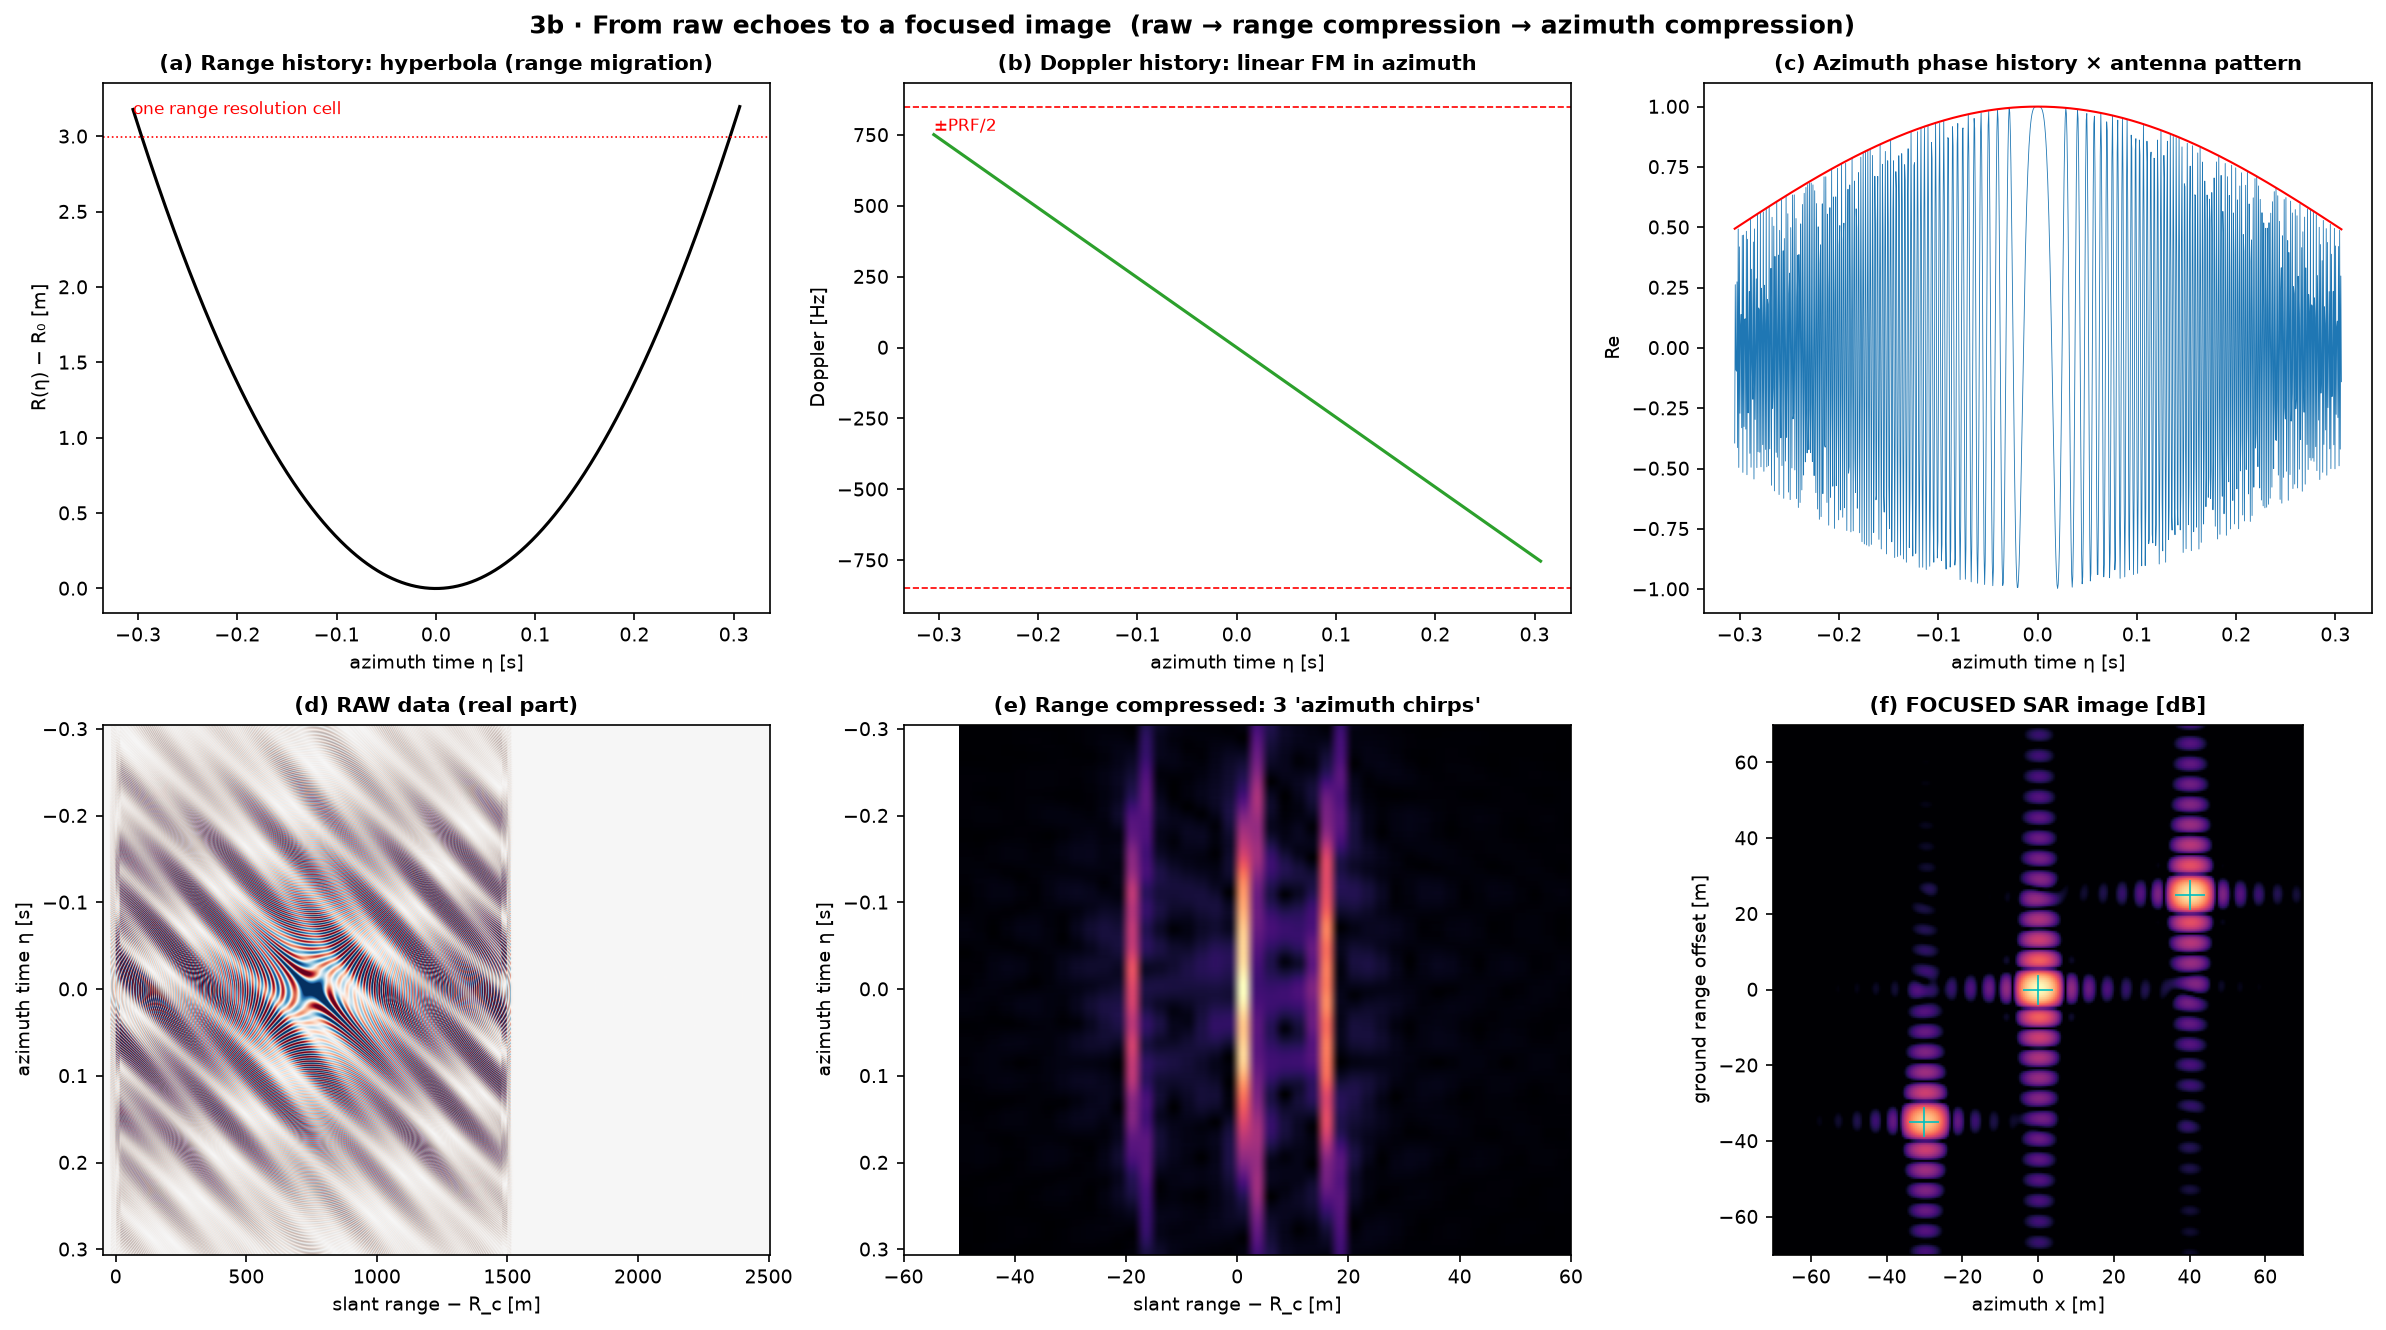
\includegraphics[width=\textwidth]{03b_signal_chain.png}
\caption[Formation of the synthetic aperture]{Formation of the synthetic aperture. Top: the beam footprint passing over three targets. Bottom: (\textbf{a}) range history; (\textbf{b}) Doppler history; (\textbf{c}) azimuth phase history weighted by the antenna pattern; (\textbf{d}) raw data; (\textbf{e}) range-compressed data; (\textbf{f}) focused image.}
\label{fig:moving}
\end{figure}
\begin{figure}[htbp]
\centering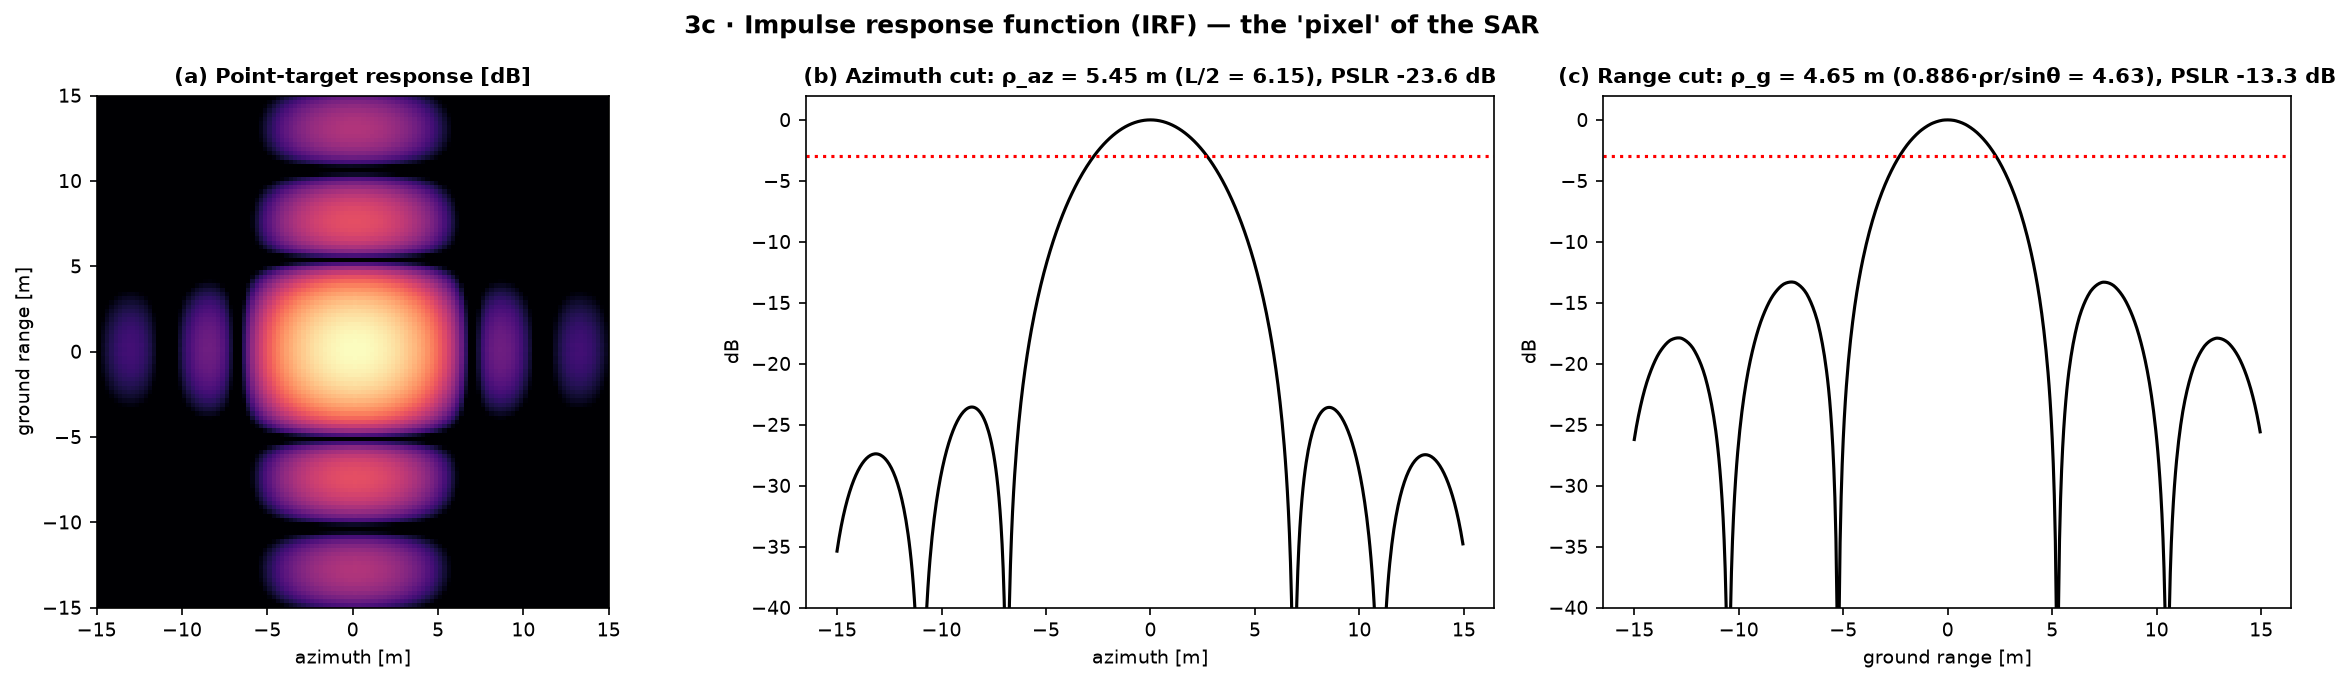
\includegraphics[width=\textwidth]{03c_impulse_response.png}
\caption[Impulse response function of the simulated SAR and its cuts in azimuth and ground range]{Impulse response function of the simulated SAR (\textbf{a}) and its cuts in azimuth (\textbf{b}) and ground range (\textbf{c}).}
\label{fig:irf}
\end{figure}

A field of 4941 scatterers with circular Gaussian amplitudes produces raw data without visible structure and a focused image that consists of fully developed speckle (Fig.~\ref{fig:flat}). The single-look intensity follows the exponential distribution, and multilooking produces a Gamma distribution whose equivalent number of looks agrees with the number of independent resolution cells averaged~\cite{goodman1976,oliver1998}. For a sinusoidal surface with uniform reflectivity per unit ground area (amplitude 12\,m, period 150\,m), the focused image still shows bright bands on the slopes facing the radar (Fig.~\ref{fig:sine}); the azimuth-averaged profile of the raw-signal simulation is reproduced by the image-domain simulation with $r=0.90$, the residual being speckle. On the $480\times480$\,m DEM patch (relief of about 550\,m; about 15{,}000 scatterers and 1100 pulses), the raw-signal simulation and focusing take about 100\,s and the image-domain simulation about 30\,ms; after $9\times9$ multilooking both agree with $r=0.97$ (Fig.~\ref{fig:dempatch}). The image-domain simulator was therefore adopted for scene-scale simulations (Fig.~\ref{fig:design}, iteration 4).

\begin{figure}[htbp]
\centering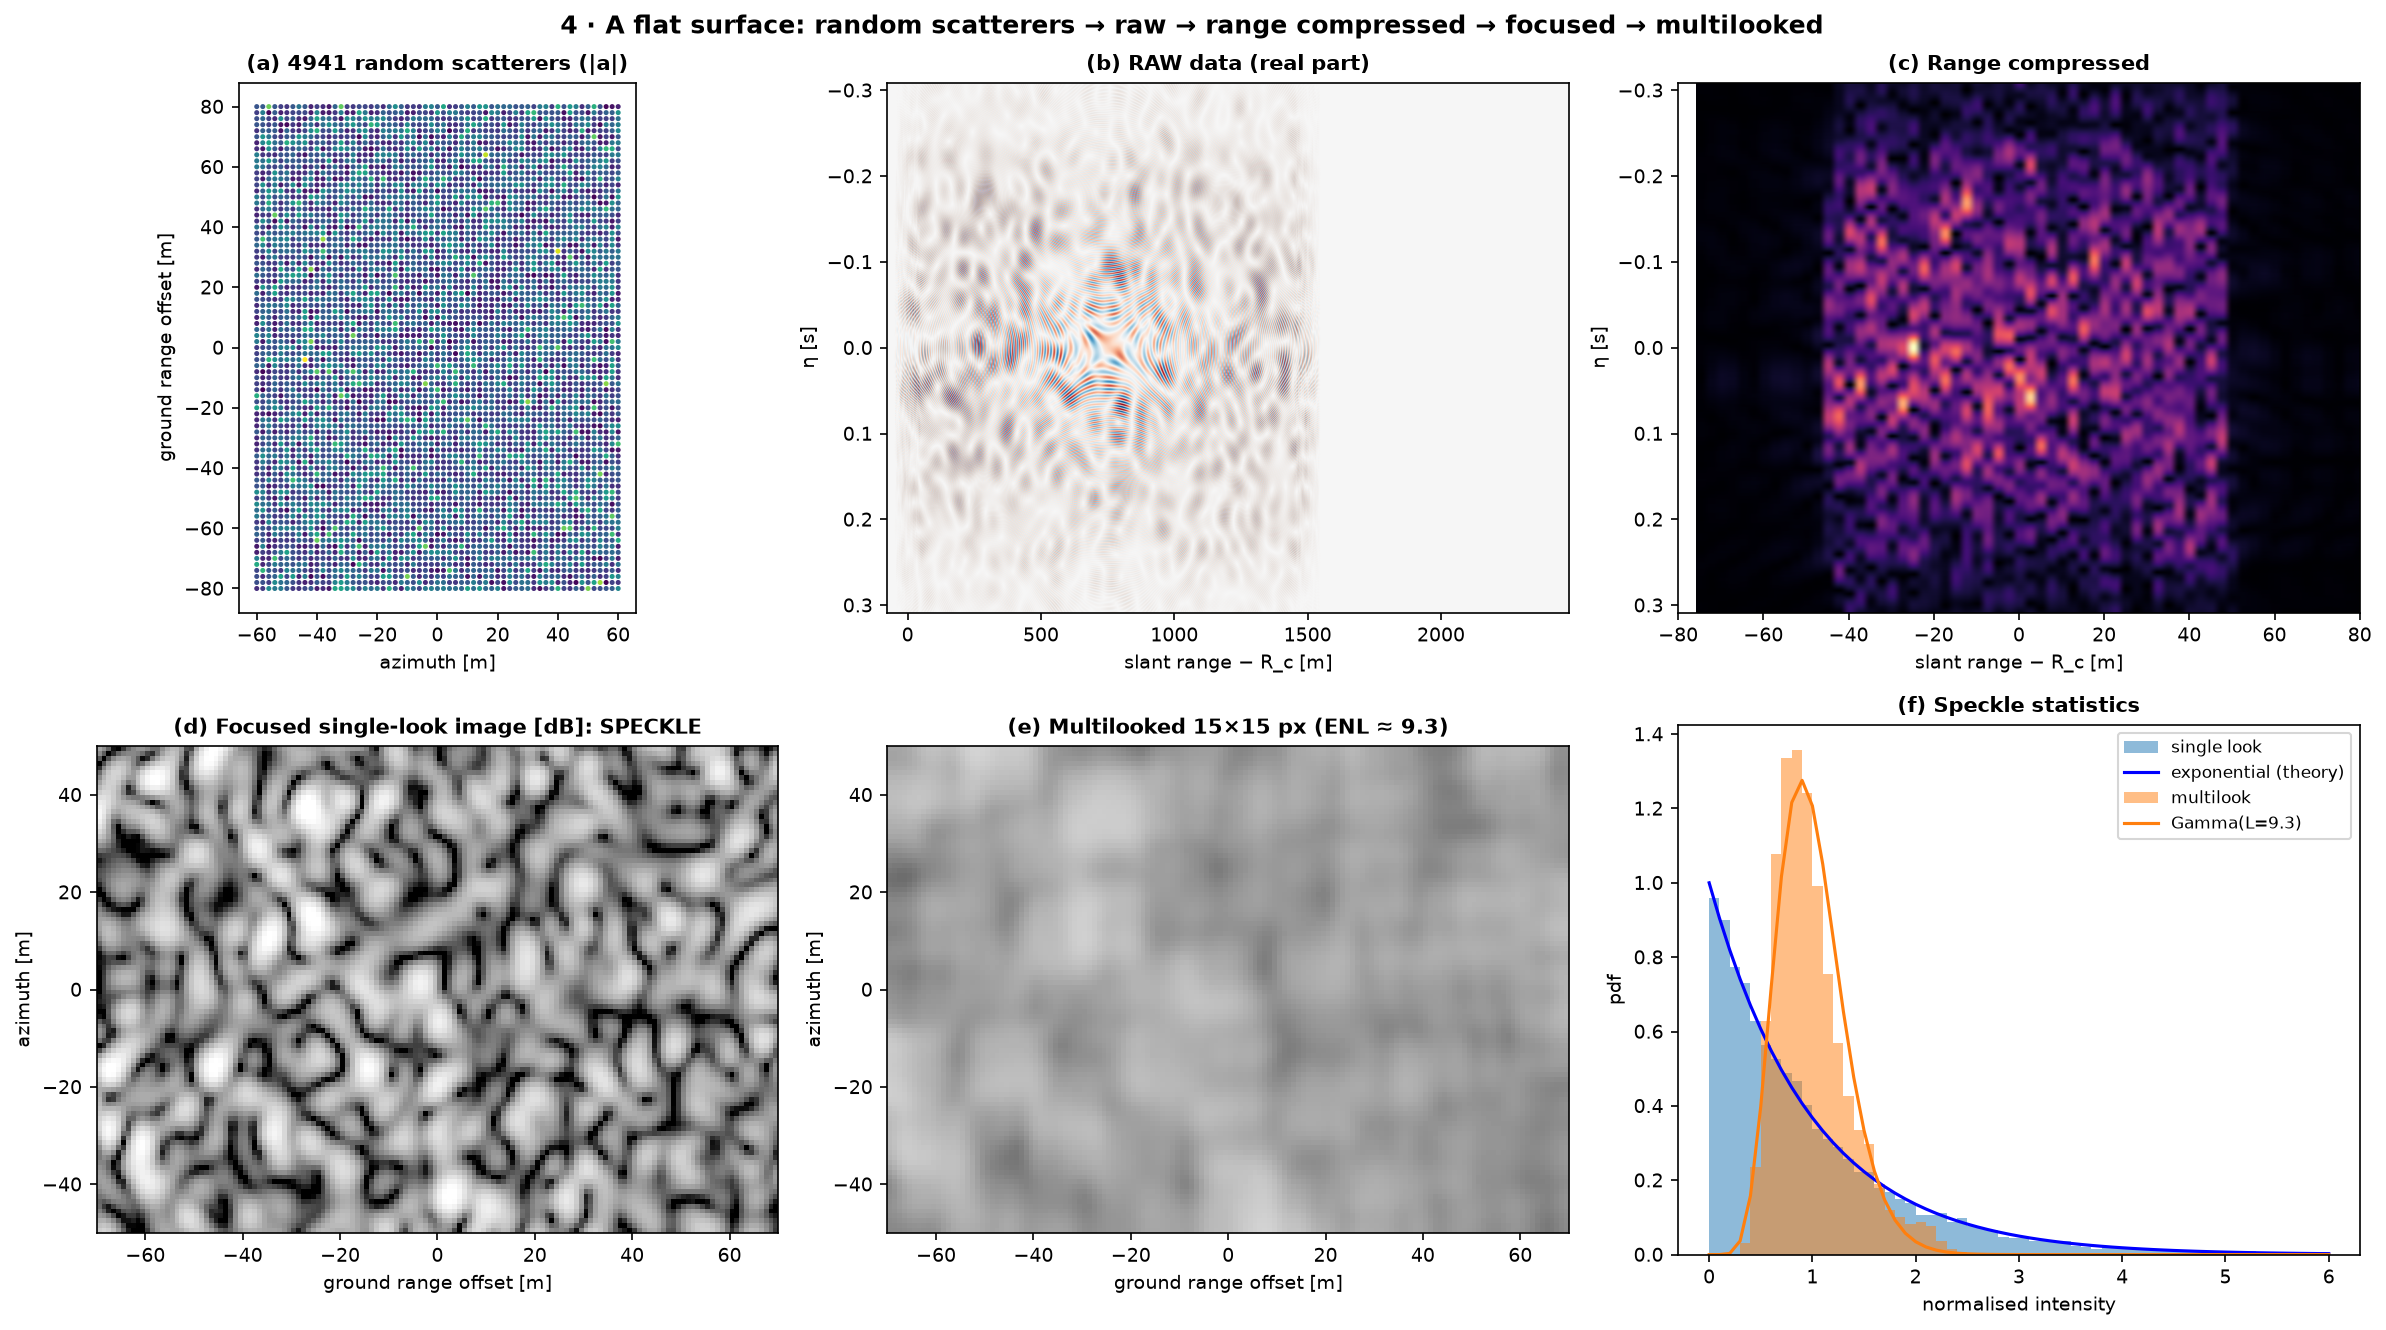
\includegraphics[width=\textwidth]{04_flat_surface_speckle.png}
\caption[Distributed scatterers]{Distributed scatterers: (\textbf{a}) random scatterer field; (\textbf{b}) raw data; (\textbf{c}) range-compressed data; (\textbf{d}) focused single-look image; (\textbf{e}) multilooked image; (\textbf{f}) intensity statistics compared with the exponential and Gamma distributions.}
\label{fig:flat}
\end{figure}
\begin{figure}[htbp]
\centering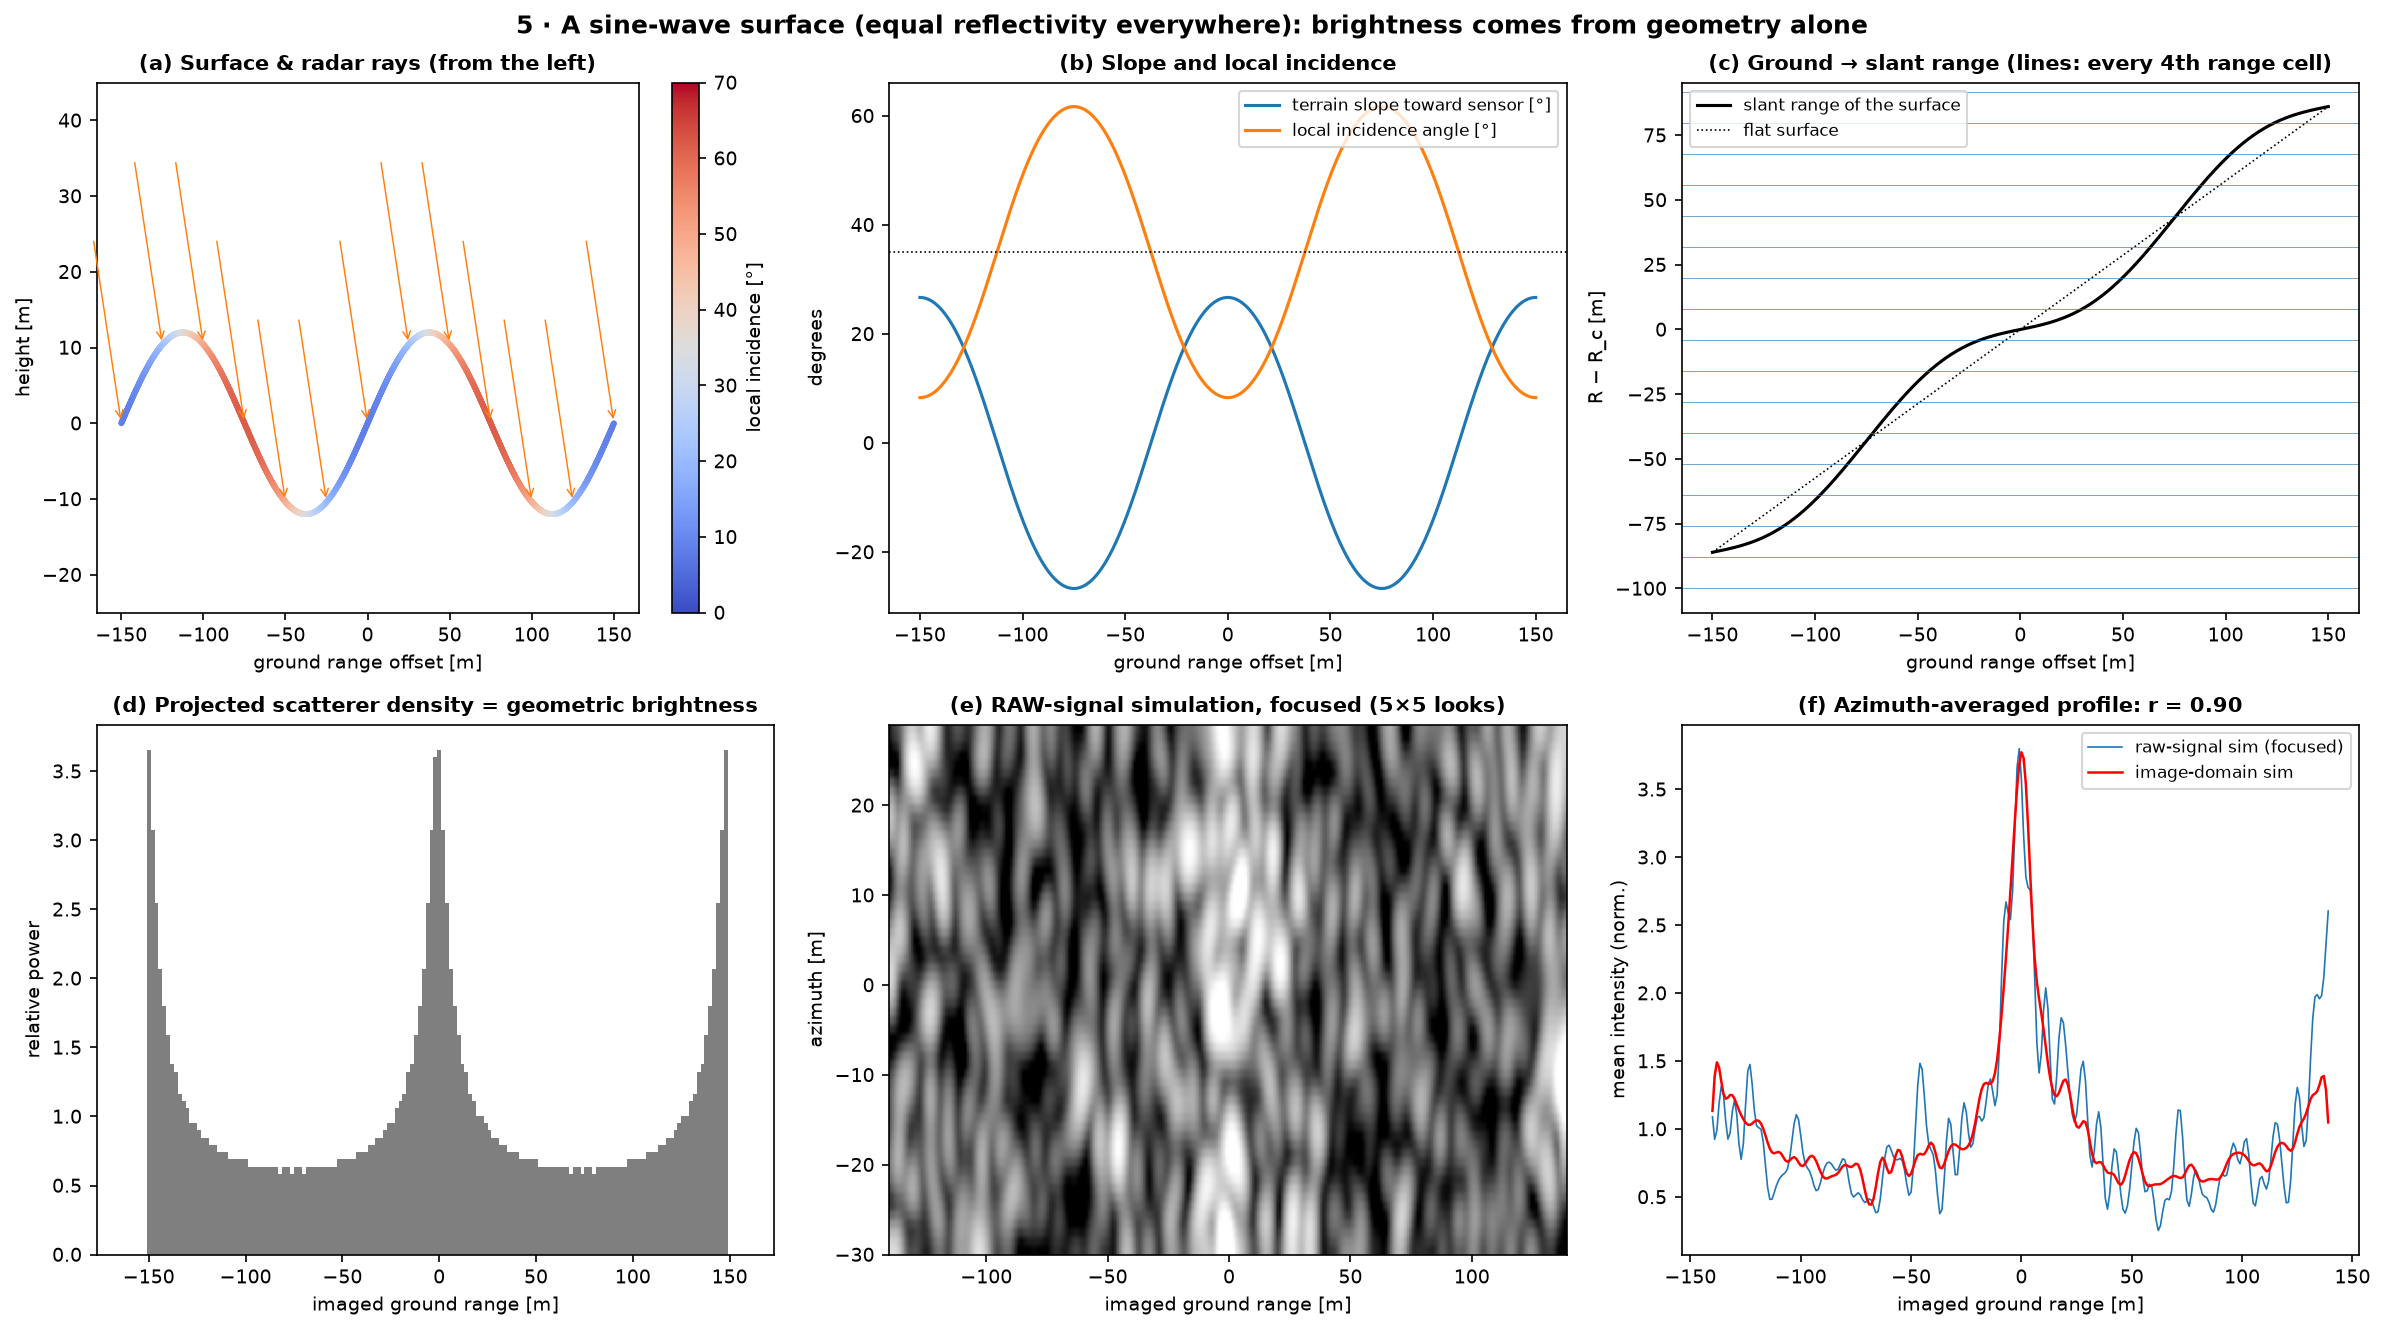
\includegraphics[width=\textwidth]{05_sine_surface.png}
\caption[Sinusoidal surface with uniform reflectivity]{Sinusoidal surface with uniform reflectivity: (\textbf{a}) profile and radar rays; (\textbf{b}) slope and local incidence angle; (\textbf{c}) ground-to-slant-range mapping; (\textbf{d}) projected scatterer density; (\textbf{e}) focused raw-signal simulation; (\textbf{f}) azimuth-averaged profiles of the raw-signal and image-domain simulations.}
\label{fig:sine}
\end{figure}
\begin{figure}[htbp]
\centering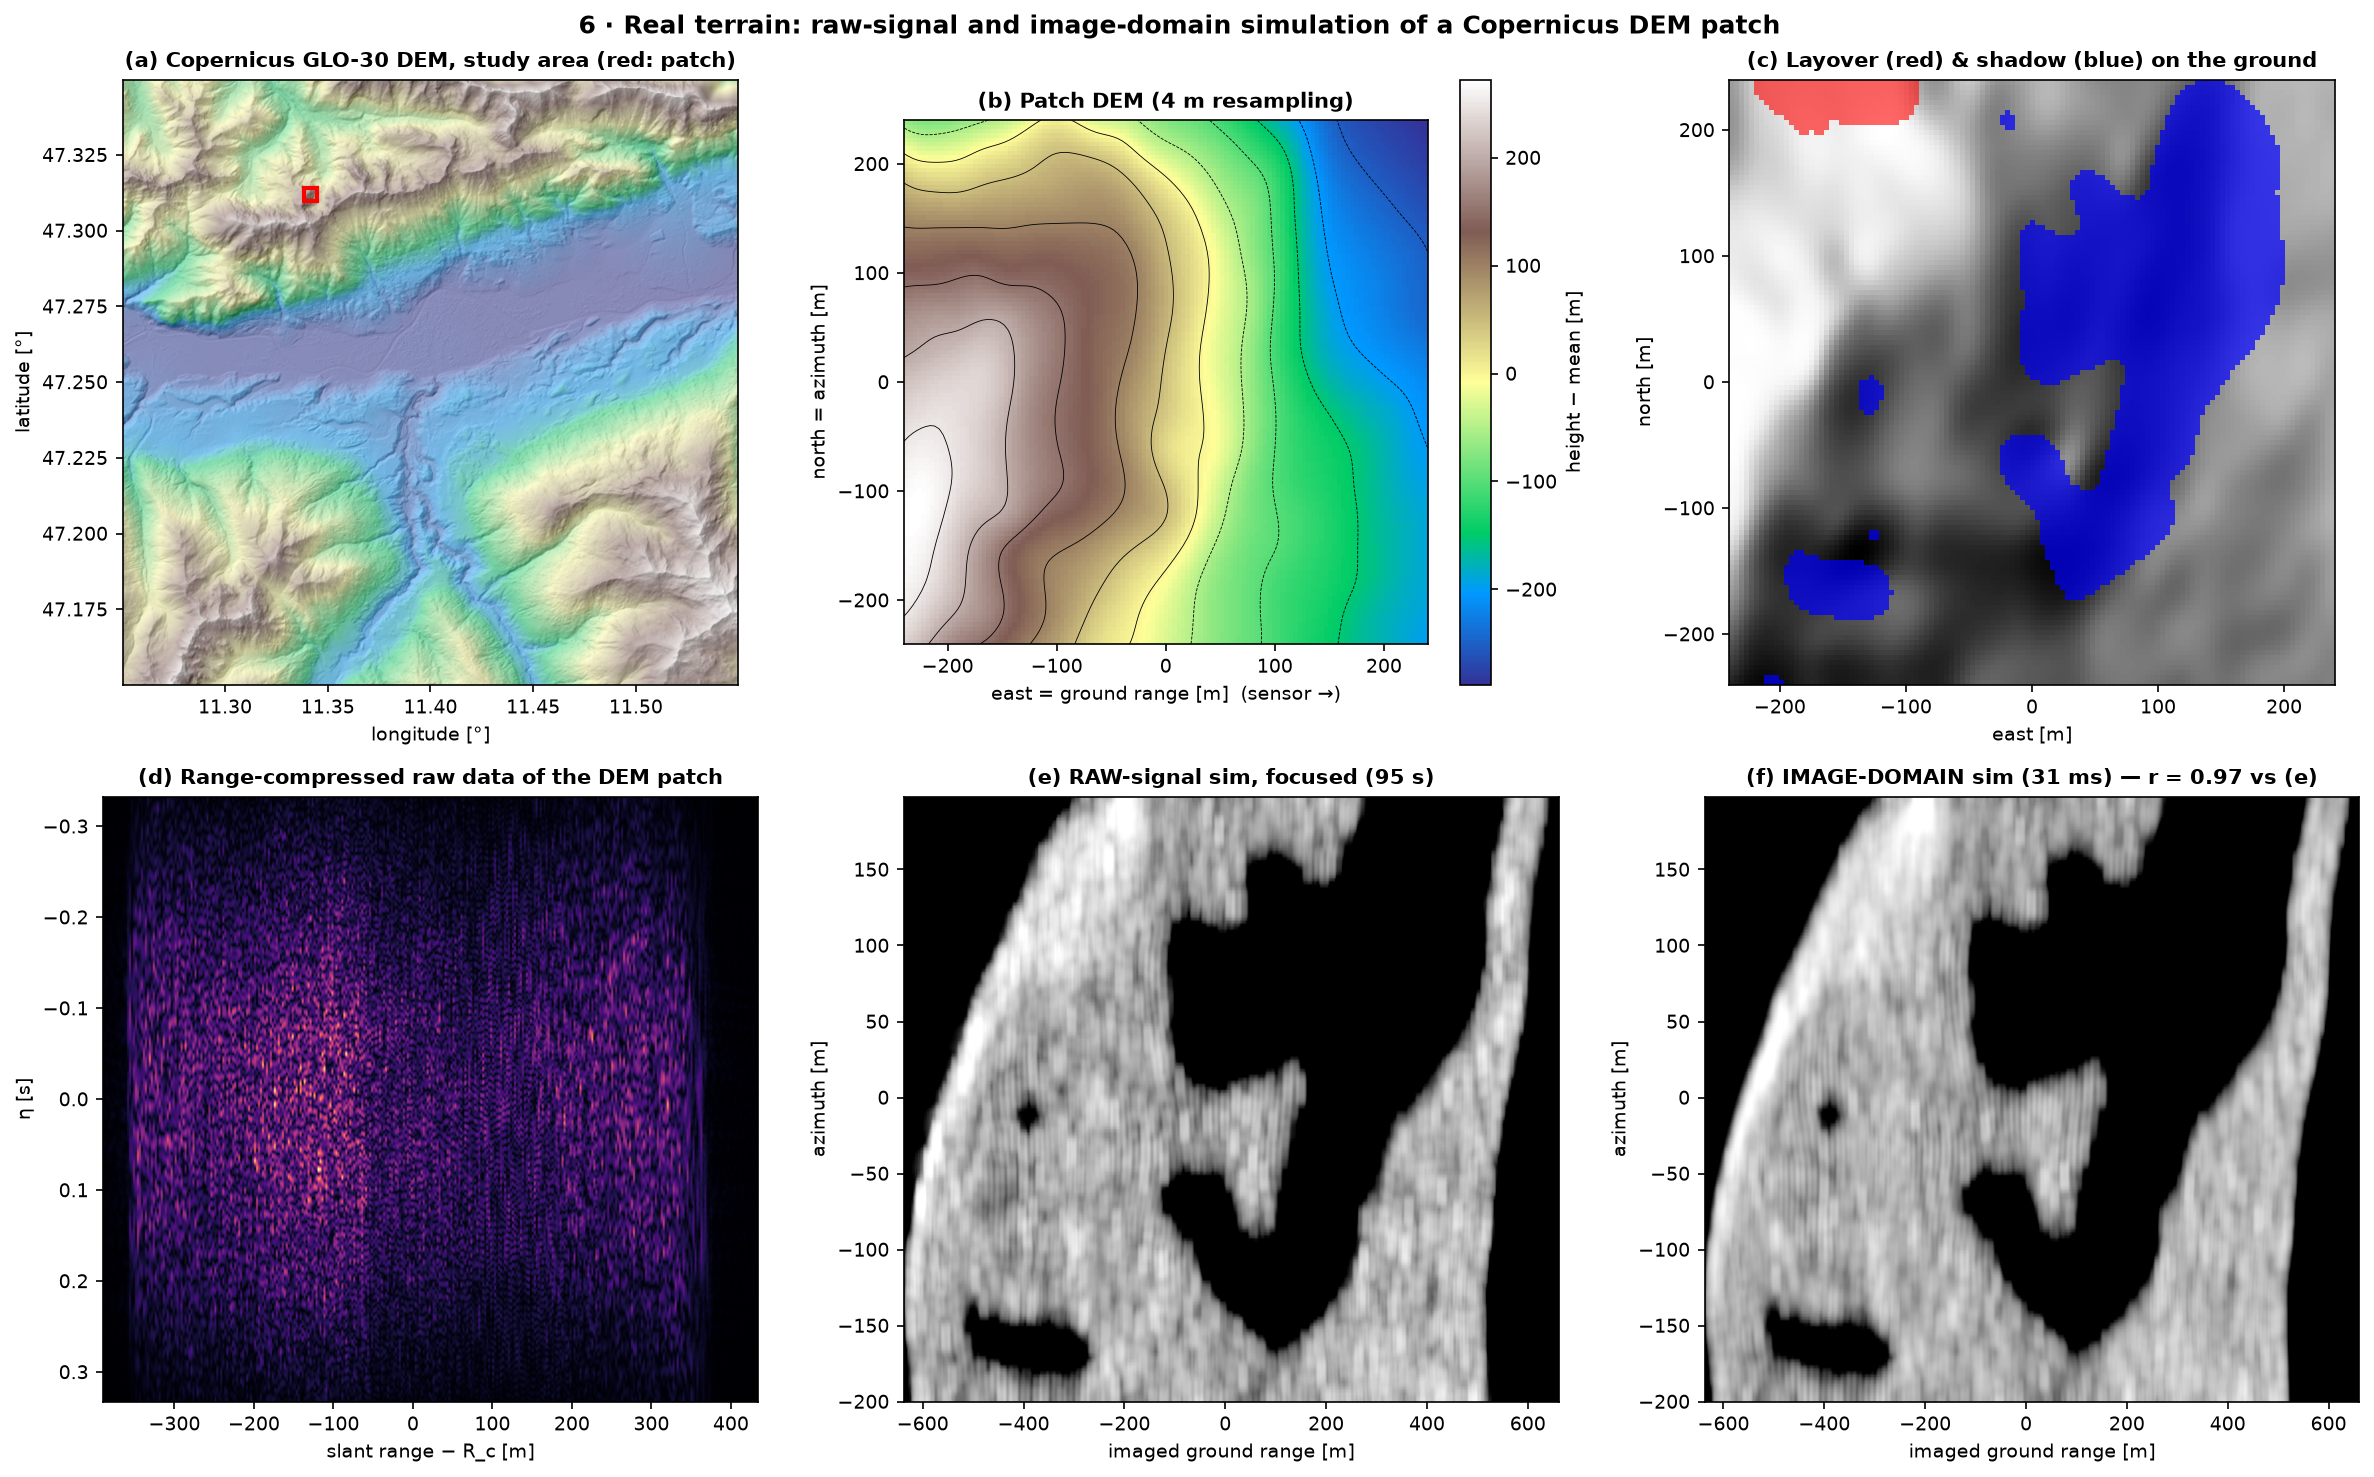
\includegraphics[width=\textwidth]{06_dem_patch_raw_vs_image_domain.png}
\caption[Copernicus DEM patch]{Copernicus DEM patch: (\textbf{a}) location; (\textbf{b}) patch DEM; (\textbf{c}) layover and shadow on the ground; (\textbf{d}) range-compressed raw data; (\textbf{e}) focused raw-signal simulation; (\textbf{f}) image-domain simulation.}
\label{fig:dempatch}
\end{figure}

\section{Geometric Distortions over the Study Site}
On a synthetic profile with a 55$^\circ$ fore-slope and a 65$^\circ$ back-slope observed at a 35$^\circ$ look angle, the shadow and layover criteria classify the fore-slope as active layover, the valley floor in front of it as passive layover, the back-slope and the plain behind it as shadow, and a gentle hill with a maximum slope of about 20$^\circ$ as foreshortened only (Fig.~\ref{fig:geomprofile}). On a $9\times9$\,km subset of the study site, layover affects 18\,\% of the area at a look angle of 20$^\circ$ and decreases to about 1\,\% at 50$^\circ$, while shadow increases from 0 to 3.4\,\% (Fig.~\ref{fig:geomdem}), which illustrates the classical trade-off in the choice of incidence angle over mountains~\cite{kropatsch1990,gelautz1998}. Fig.~\ref{fig:radio} builds the simulated image in the order of the physics: local incidence angle, $\sigz(\theta_{loc})$, illuminated area, their product, speckle and multilooking. The geometric term alone, i.e., the illuminated area per pixel, already reproduces most of the image structure.

\begin{figure}[htbp]
\centering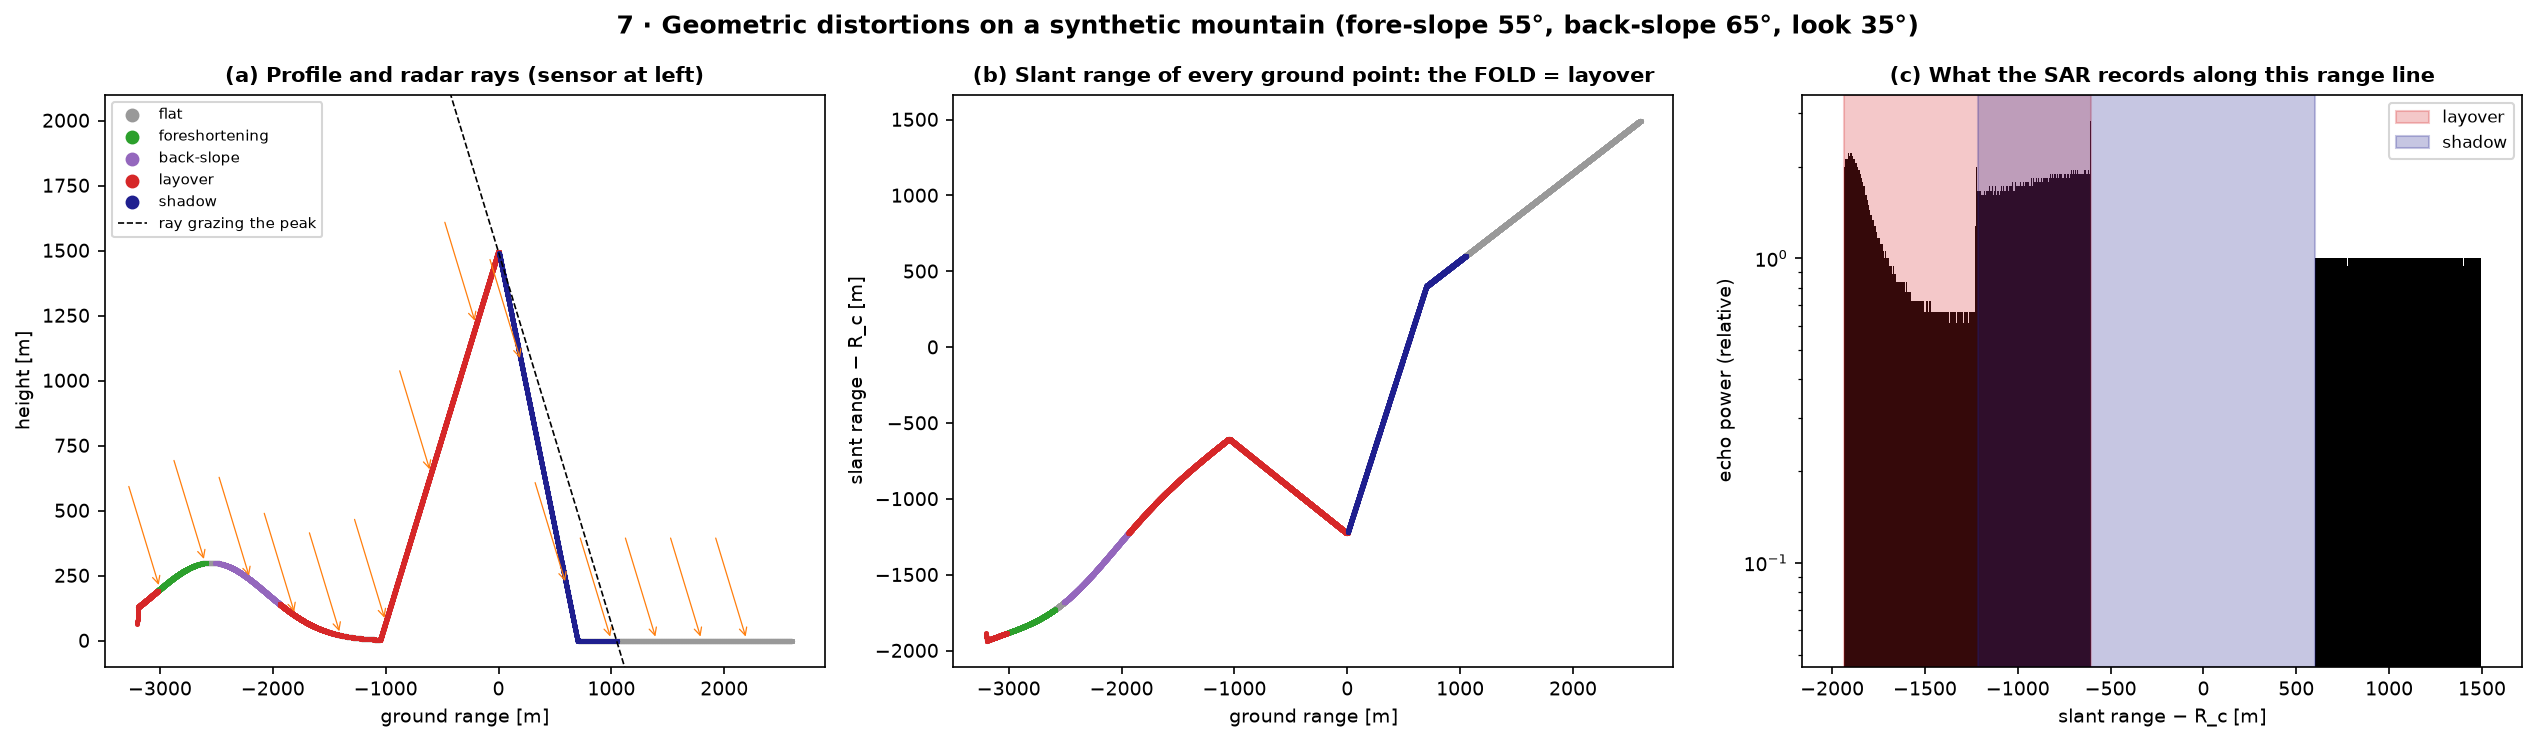
\includegraphics[width=\textwidth]{07_geometric_distortions_profile.png}
\caption[Geometric distortions along a synthetic profile]{Geometric distortions along a synthetic profile: (\textbf{a}) classification and radar rays; (\textbf{b}) slant range of every ground point, where the fold indicates layover; (\textbf{c}) echo power recorded along the range line.}
\label{fig:geomprofile}
\end{figure}
\begin{figure}[htbp]
\centering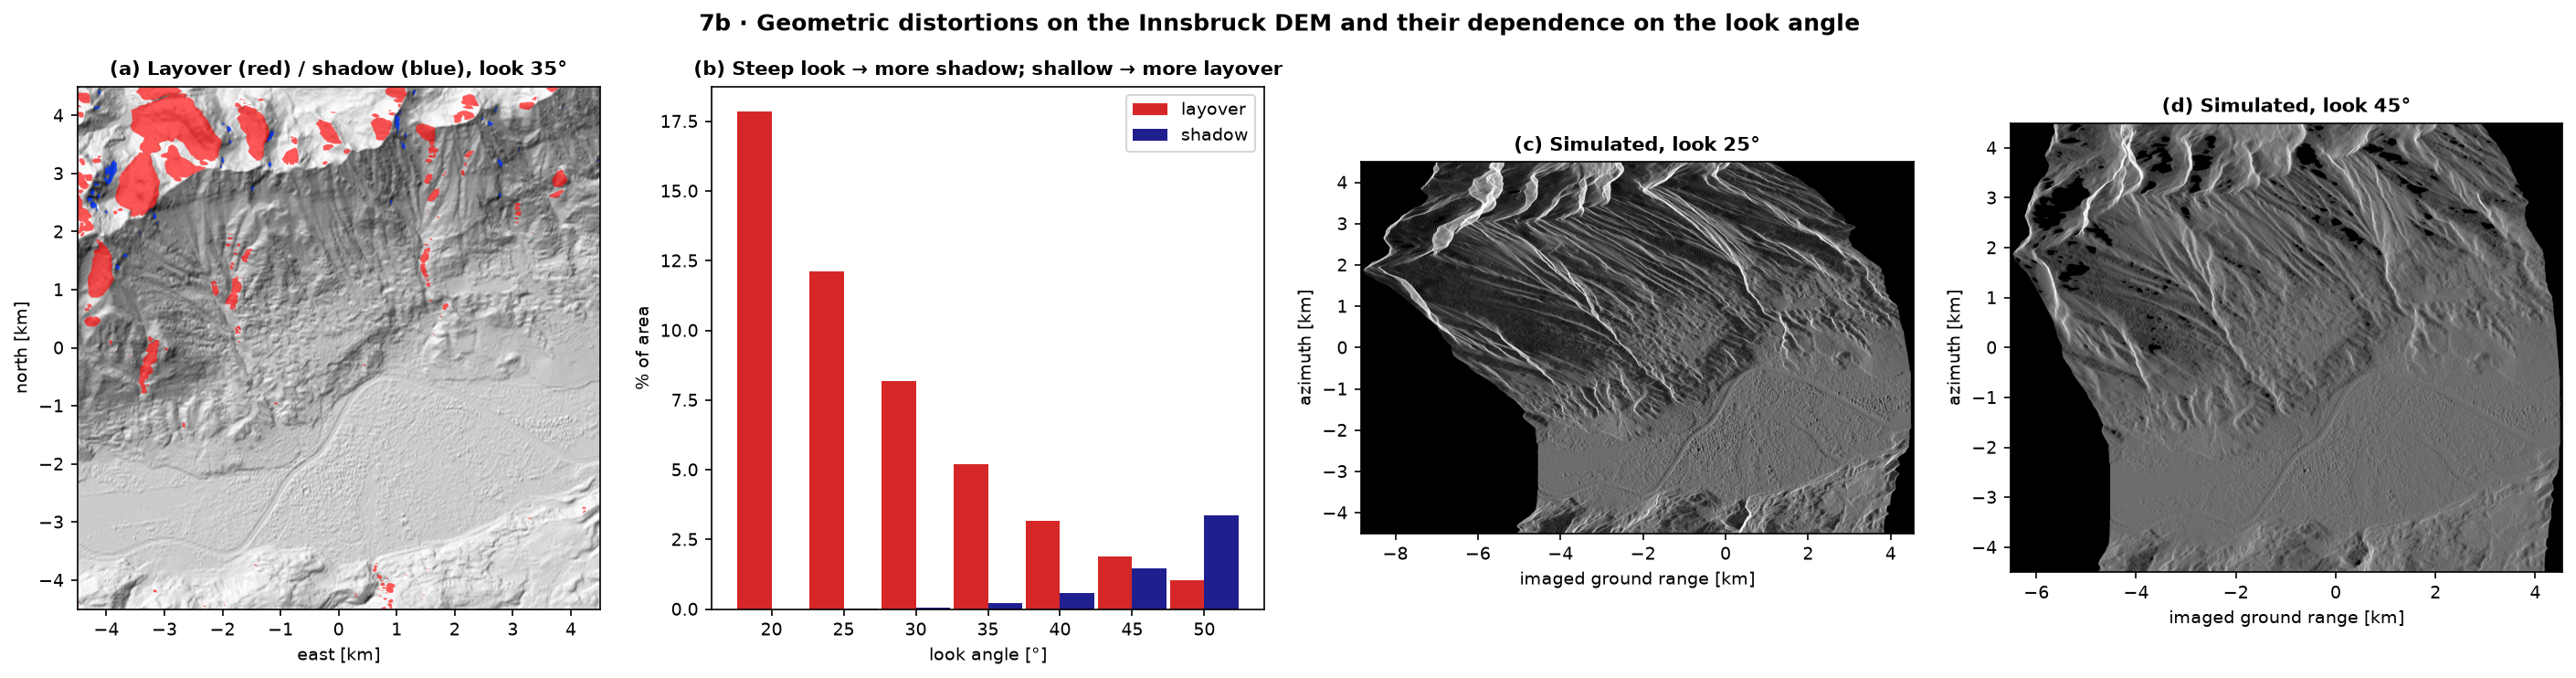
\includegraphics[width=\textwidth]{07b_geometric_distortions_dem.png}
\caption[Layover and shadow over a $9\times9$\,km subset of the study site, their fraction as a function of the look angle, and simulated images at look angles of 25$^\circ$ and 45$^\circ$]{Layover and shadow over a $9\times9$\,km subset of the study site (\textbf{a}), their fraction as a function of the look angle (\textbf{b}), and simulated images at look angles of 25$^\circ$ (\textbf{c}) and 45$^\circ$ (\textbf{d}).}
\label{fig:geomdem}
\end{figure}
\begin{figure}[htbp]
\centering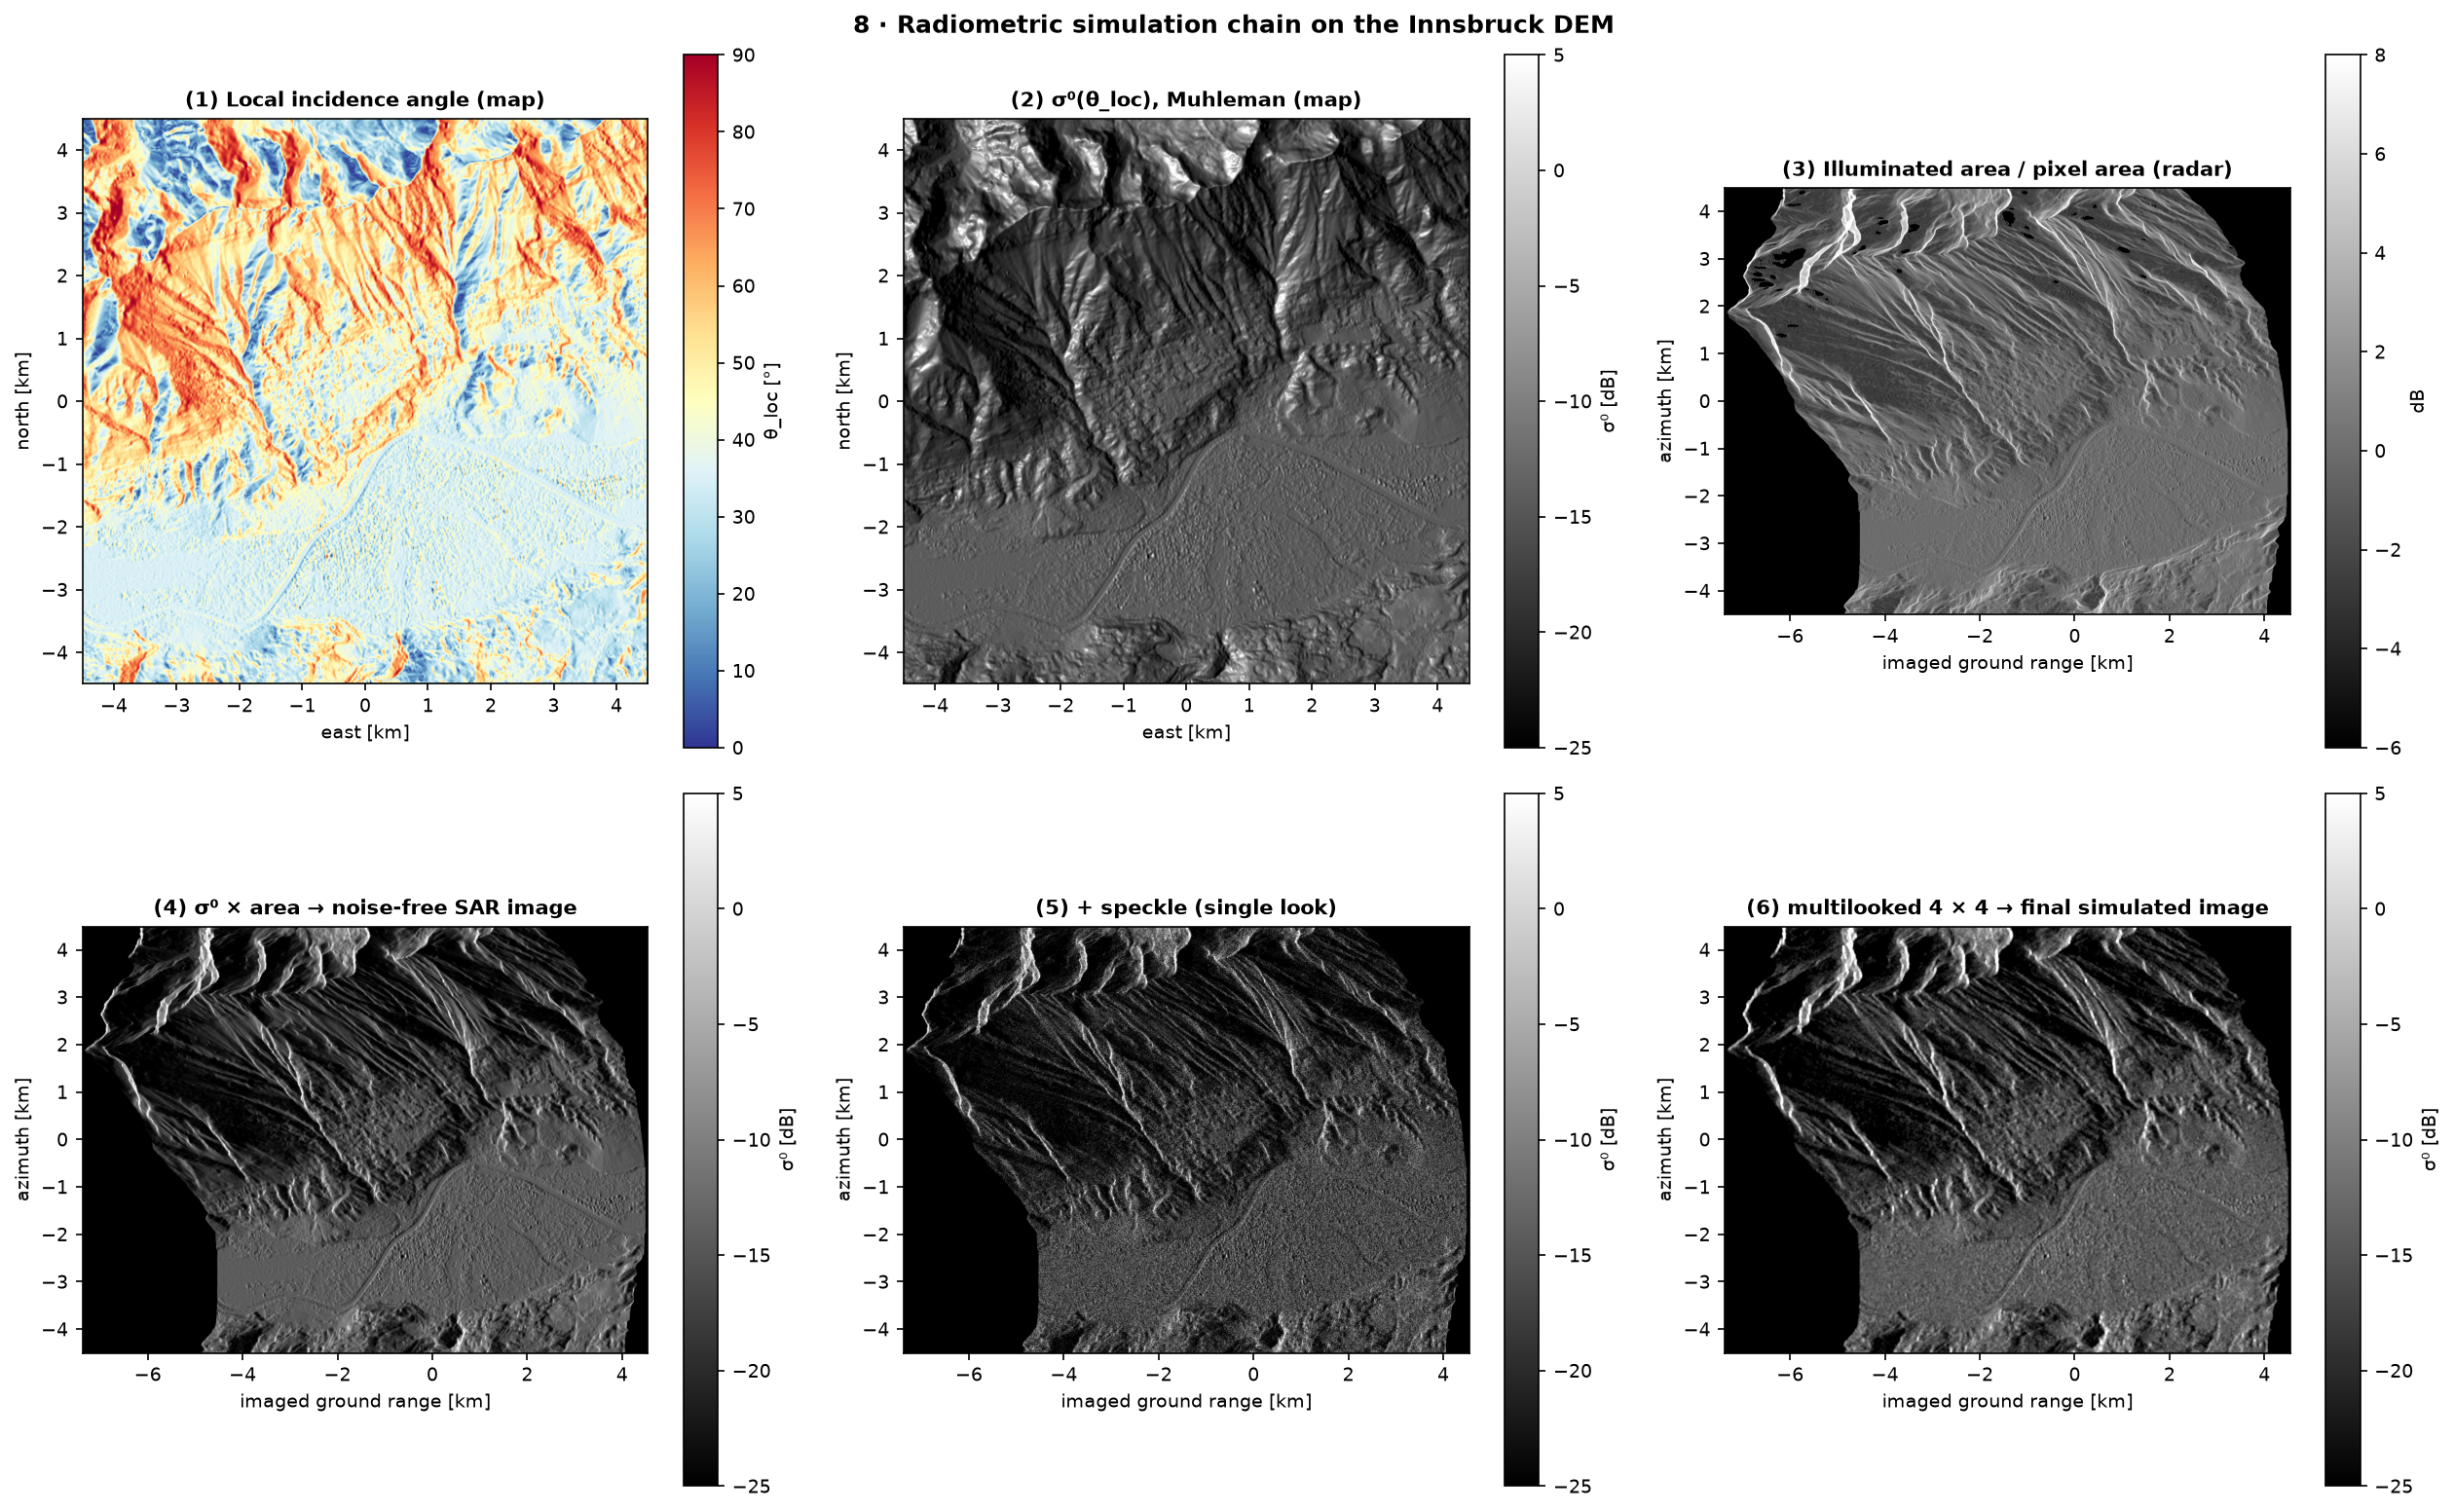
\includegraphics[width=\textwidth]{08b_radiometric_chain.png}
\caption[Radiometric simulation chain]{Radiometric simulation chain: (\textbf{1}) local incidence angle; (\textbf{2}) $\sigz$ from Muhleman's law in map geometry; (\textbf{3}) illuminated area per pixel in radar geometry; (\textbf{4}) noise-free simulated image; (\textbf{5}) single-look speckle; (\textbf{6}) multilooked image.}
\label{fig:radio}
\end{figure}

\section{Geocoding Accuracy}
\label{sec:res-geo}
With the valid-from rule for the SRGR polynomials, the range-Doppler geocoding reproduces the geolocation grid of both products to \geoDpixMax{} pixels in range, \geoDtMax{} ms in zero-Doppler time (\geoDlineMax{} lines) and \geoDRmax{} mm in slant range over all \nGrid{} tie points of each scene (Fig.~\ref{fig:geomval}a). Linear interpolation between the polynomial sets increased the maximum range error to 3.3 pixels (Fig.~\ref{fig:design}, iteration 5). The line numbers tabulated in the geolocation grid are nominal and deviate by up to 0.2 lines from the zero-Doppler times listed for the same points; the latter must be used for validation.

\section{Comparison with Sentinel-1 and the Backscatter Law}
Fig.~\ref{fig:realsim} compares the real ascending image with the simulation. Ridges, valleys, bright fore-slopes, layover bands and black shadows of the real image are reproduced at the right positions, while the urbanised valley floor appears as a uniform surface in the simulation. Table~\ref{tab:models} and Fig.~\ref{fig:models} summarise the agreement for the five backscatter laws. The constant law, which only contains the illuminated-area term, already reaches $r=0.53$. Laws that decrease with $\theta_{loc}$ improve the agreement substantially, but no single law is best for every metric: Muhleman's law gives the highest correlation ($r=\rMuAsc$), the Lambert and fitted laws the highest SSIM, and the cosine law the lowest RMSE. The fitted law has an exponent $n=\nFit$ and $10\log_{10}k=\kFitDb$\,dB, i.e., the data select Lambert's law (Fig.~\ref{fig:fit}). It describes the median real $\sigz$ well between 10$^\circ$ and 80$^\circ$, whereas at small local incidence angles the real backscatter rises more steeply, which Muhleman's law captures; these few very bright pixels weigh heavily in the Pearson correlation. The interquartile range of the real $\sigz$ at a given $\theta_{loc}$ is about 5\,dB, which indicates that land cover, rather than the angular law, limits the agreement.

\begin{figure}[htbp]
\centering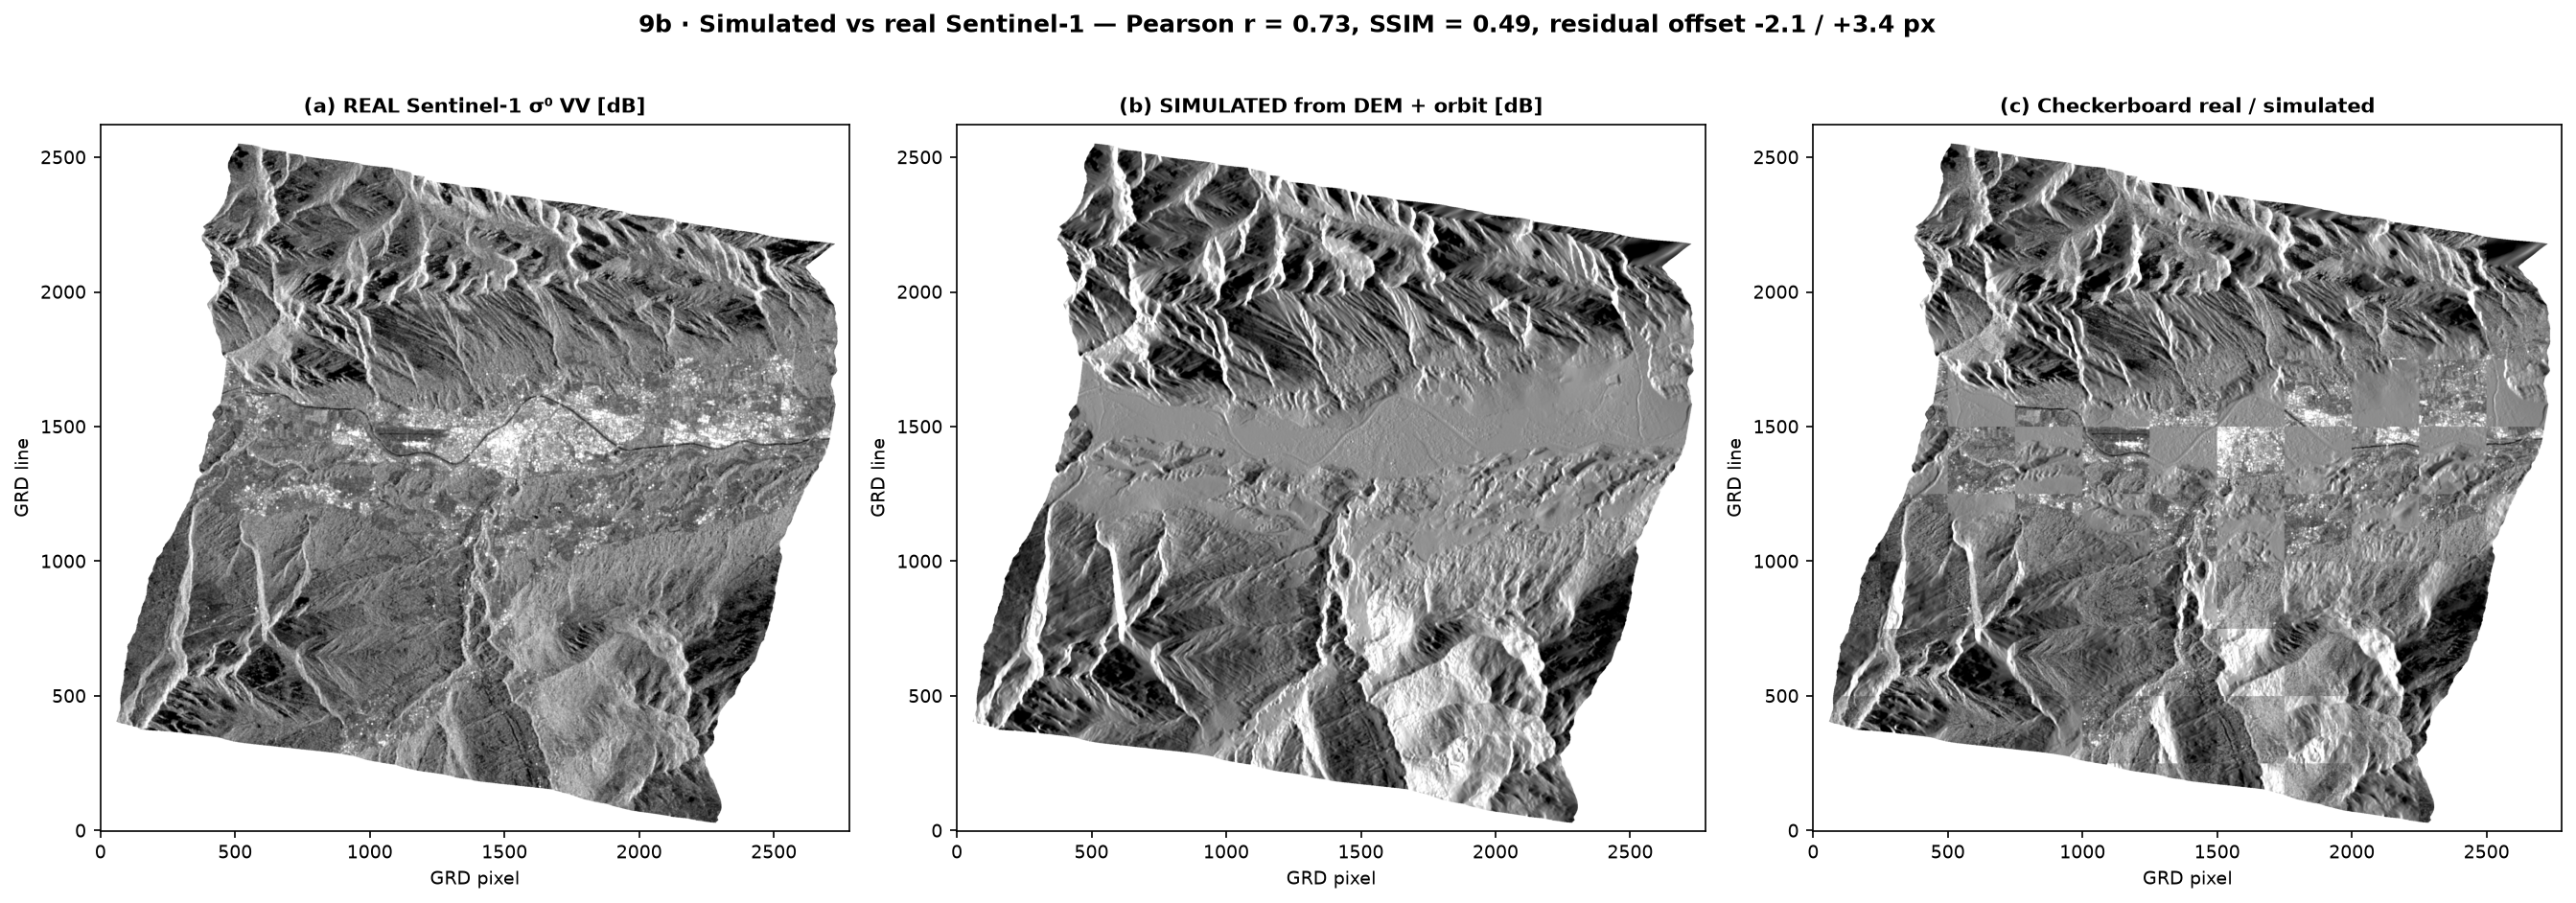
\includegraphics[width=\textwidth]{09b_real_vs_simulated.png}
\caption[Real Sentinel-1 $\sigz$, simulation with Muhleman's law and a checkerboard of both; ascending scene, radar geometry]{Real Sentinel-1 $\sigz$ (\textbf{a}), simulation with Muhleman's law (\textbf{b}) and a checkerboard of both (\textbf{c}); ascending scene, radar geometry.}
\label{fig:realsim}
\end{figure}

\begin{table}[htbp]
\caption[Agreement between the real and the simulated ascending image for five backscatter laws ($5\times5$ multilook, dB)]{Agreement between the real and the simulated ascending image for five backscatter laws ($5\times5$ multilook, dB). The level offset is the constant added to the law to calibrate its absolute level.}
\label{tab:models}
\centering\small
\begin{tabular}{lrrrrr}\toprule
 Backscatter model & Pearson $r$ & Spearman $\rho$ & SSIM & RMSE [dB] & level offset [dB]\\\midrule
Constant & 0.534 & 0.739 & 0.377 & 3.83 & -0.6 \\
$\cos\theta_{loc}$ & 0.663 & 0.767 & 0.467 & 3.72 & -8.3 \\
$\cos^2\theta_{loc}$ (Lambert) & 0.703 & 0.762 & 0.509 & 4.44 & -6.1 \\
Muhleman & 0.734 & 0.757 & 0.494 & 4.58 & 7.6 \\
Fitted $k\cos^{1.98}\theta_{loc}$ & 0.710 & 0.761 & 0.508 & 4.29 & -1.4 \\
\bottomrule\end{tabular}

\end{table}

\begin{figure}[htbp]
\centering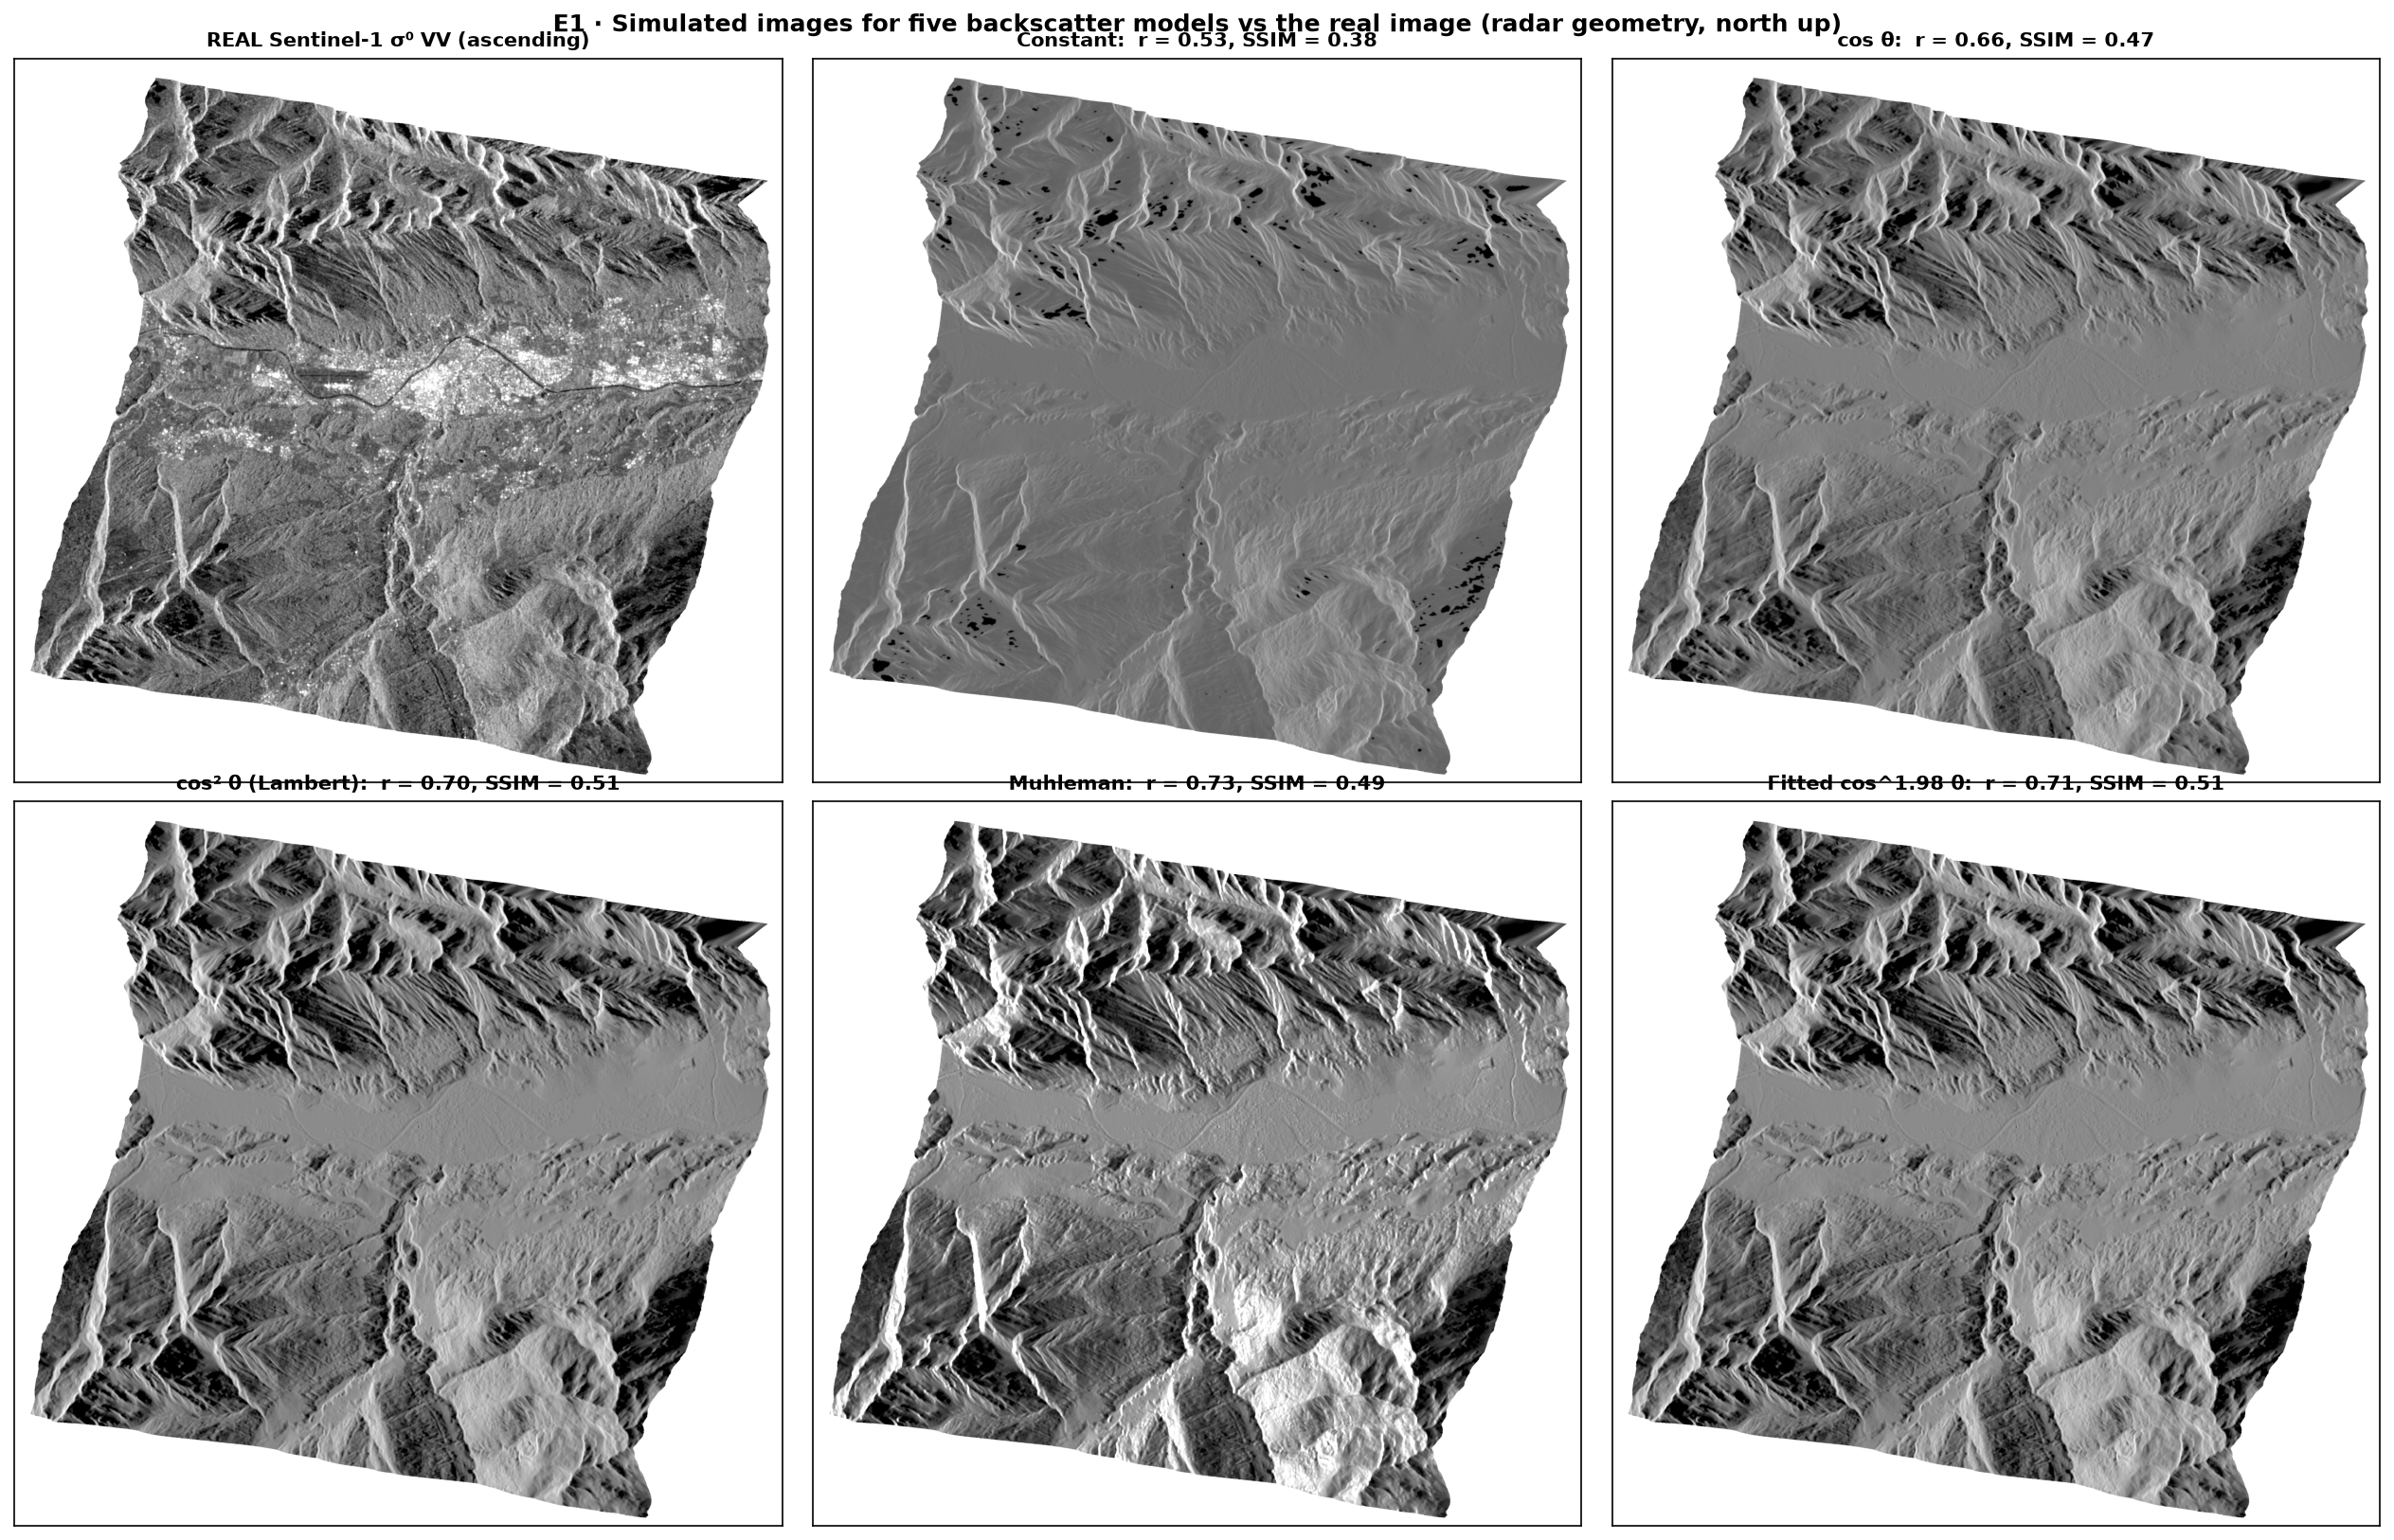
\includegraphics[width=\textwidth]{p1_models_images.png}
\caption[Real ascending image and simulations with the five backscatter laws (radar geometry, north up)]{Real ascending image and simulations with the five backscatter laws (radar geometry, north up).}
\label{fig:models}
\end{figure}
\begin{figure}[htbp]
\centering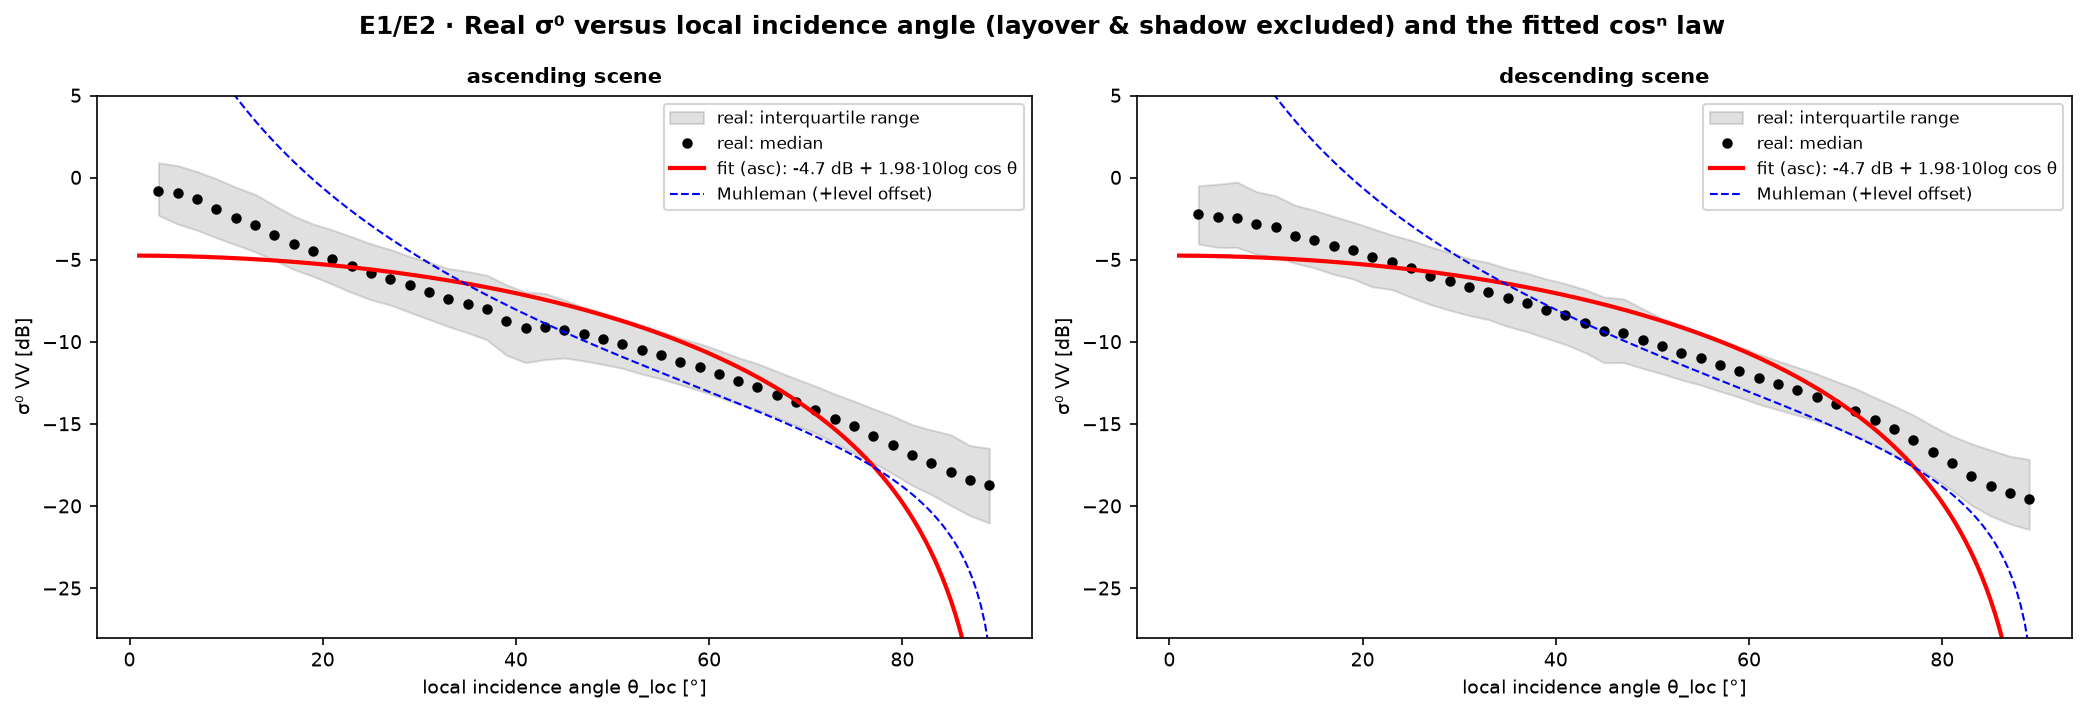
\includegraphics[width=\textwidth]{p2_fitted_model.png}
\caption[Real $\sigz$ as a function of the local incidence angle for the ascending and descending scenes, excluding layover and shadow, with the $\cos^n$ law fitted on the ascending scene and Muhleman's law]{Real $\sigz$ as a function of the local incidence angle for the ascending (\textbf{a}) and descending (\textbf{b}) scenes, excluding layover and shadow, with the $\cos^n$ law fitted on the ascending scene and Muhleman's law.}
\label{fig:fit}
\end{figure}

\section{Second Viewing Geometry}
The descending scene looks west, so that layover and shadow move to the opposite slopes (Fig.~\ref{fig:ascdesc}). Applying the law fitted on the ascending scene without any change yields $r=\rDesc$, $\rho=\rhoDesc$, SSIM\,$=\ssimDesc$ and RMSE\,$=\rmseDesc$\,dB, compared with $r=\rAsc$, $\rho=\rhoAsc$, SSIM\,$=\ssimAsc$ and RMSE\,$=\rmseAsc$\,dB on the ascending scene (Fig.~\ref{fig:scatter}). A refit on the descending scene gives $n=\nRefitDesc$. The empirical law therefore transfers between the two viewing geometries; it describes the terrain rather than the acquisition.

\begin{figure}[htbp]
\centering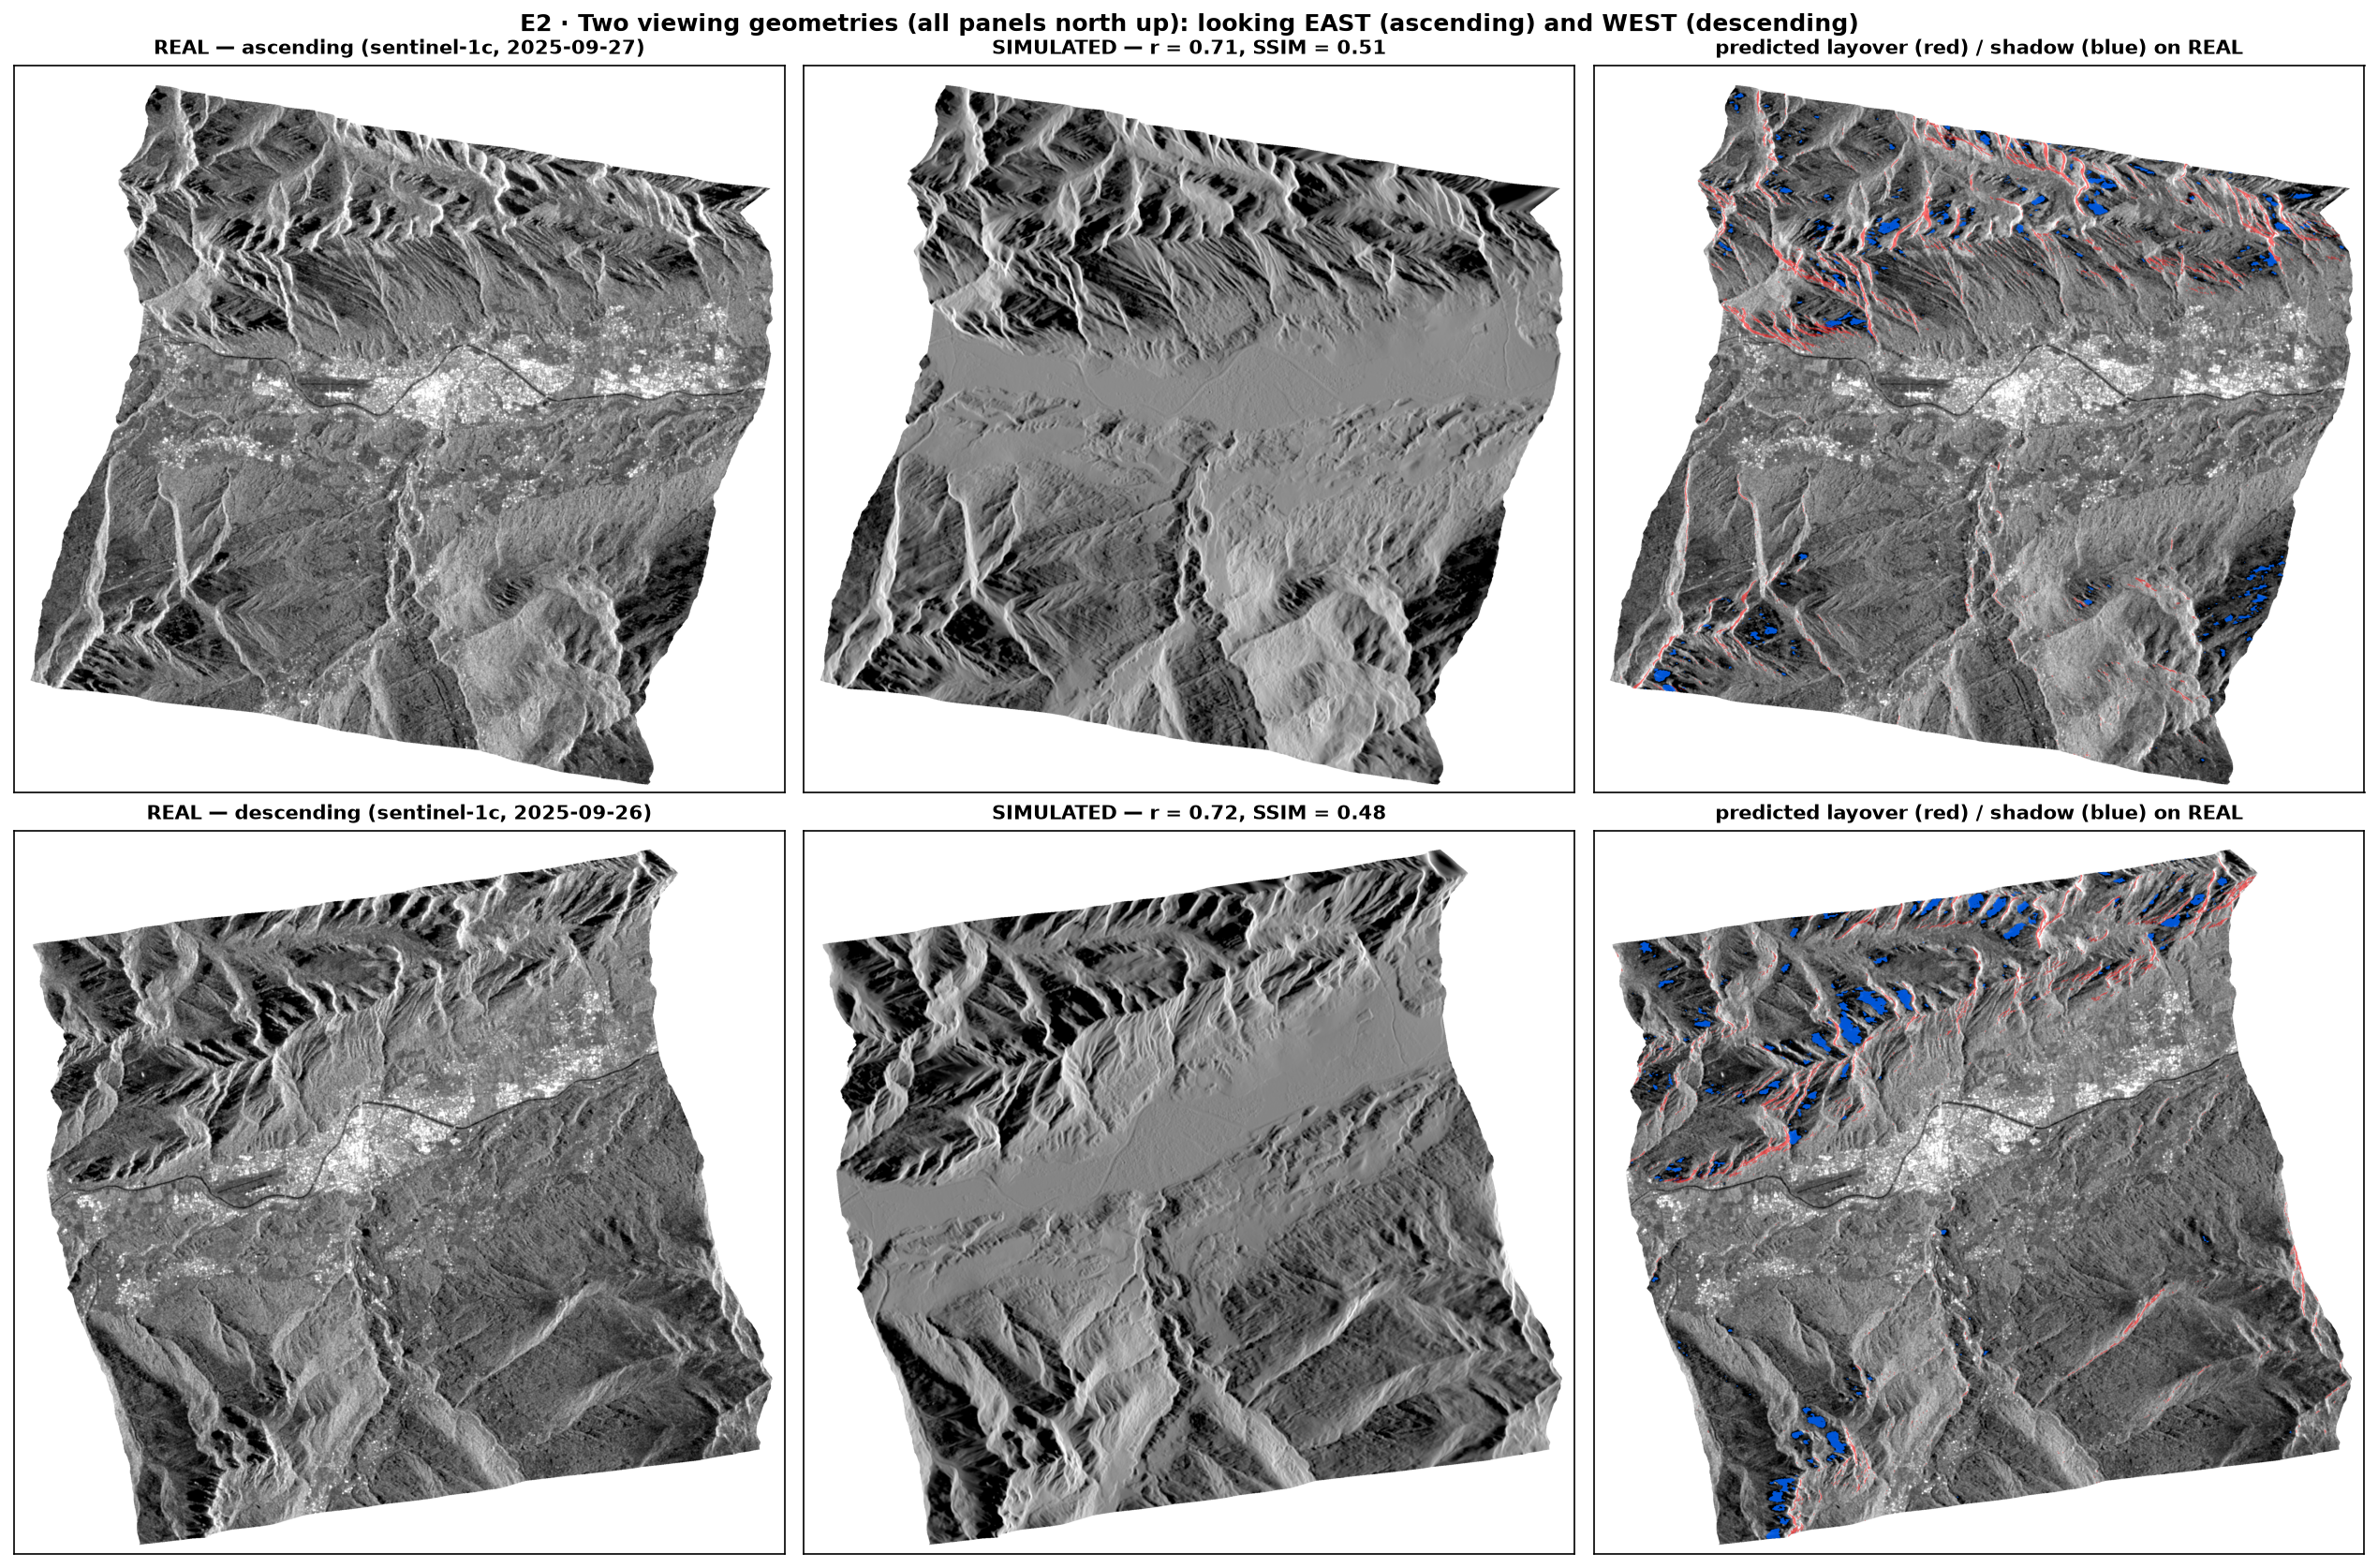
\includegraphics[width=\textwidth]{p3_ascending_descending.png}
\caption[Real and simulated images, and predicted layover (red) and shadow (blue) drawn on the real image, for the ascending (top, looking east) and descending (bottom, looking west) scenes; all panels north up]{Real and simulated images, and predicted layover (red) and shadow (blue) drawn on the real image, for the ascending (top, looking east) and descending (bottom, looking west) scenes; all panels north up.}
\label{fig:ascdesc}
\end{figure}
\begin{figure}[htbp]
\centering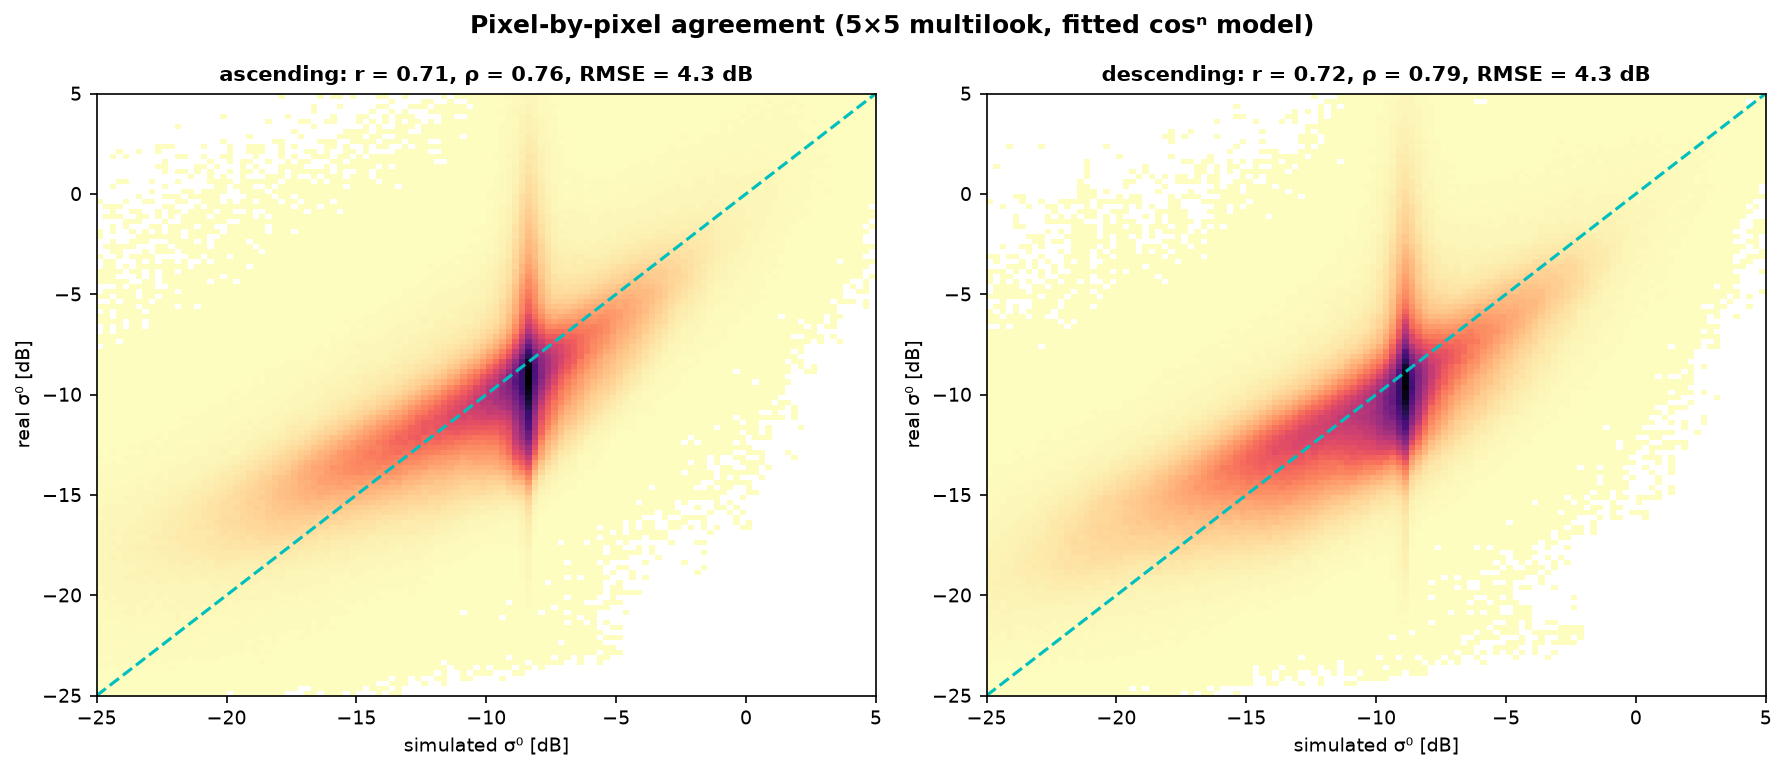
\includegraphics[width=0.86\textwidth]{p8_scatter.png}
\caption[Pixel-by-pixel comparison of real and simulated $\sigz$ for both scenes with the fitted law]{Pixel-by-pixel comparison of real and simulated $\sigz$ for both scenes with the fitted law.}
\label{fig:scatter}
\end{figure}

\section{Validation of the Predicted Distortion Classes}
Table~\ref{tab:classes} and Fig.~\ref{fig:geomval} test the predicted distortion classes against the real images. Pixels predicted to be in shadow are the darkest, with a median of $-21.0$\,dB (ascending) and $-22.0$\,dB (descending), i.e., at the noise floor of the sensor, since thermal noise was not removed. Pixels predicted to be in layover ($-3.5$ and $-3.9$\,dB) or strongly foreshortened ($-4.5$ and $-5.1$\,dB) are the brightest, about 7\,dB above the remaining terrain. The ordering of the classes is identical in both geometries.

\begin{table}[htbp]
\caption[Real $\sigz$ inside the distortion classes predicted by the simulation]{Real $\sigz$ inside the distortion classes predicted by the simulation.}
\label{tab:classes}
\centering\small
\begin{tabular}{lrrrr}\toprule
 & \multicolumn{2}{c}{ascending} & \multicolumn{2}{c}{descending}\\
Predicted class & pixels & median $\sigma^0$ [dB] & pixels & median $\sigma^0$ [dB]\\\midrule
shadow & 47k & -21.0 & 66k & -22.0 \\
layover & 82k & -3.5 & 61k & -3.9 \\
foreshortened (area > 2x) & 228k & -4.5 & 220k & -5.1 \\
other terrain & 4525k & -10.8 & 4576k & -11.5 \\
\bottomrule\end{tabular}

\end{table}
\begin{figure}[htbp]
\centering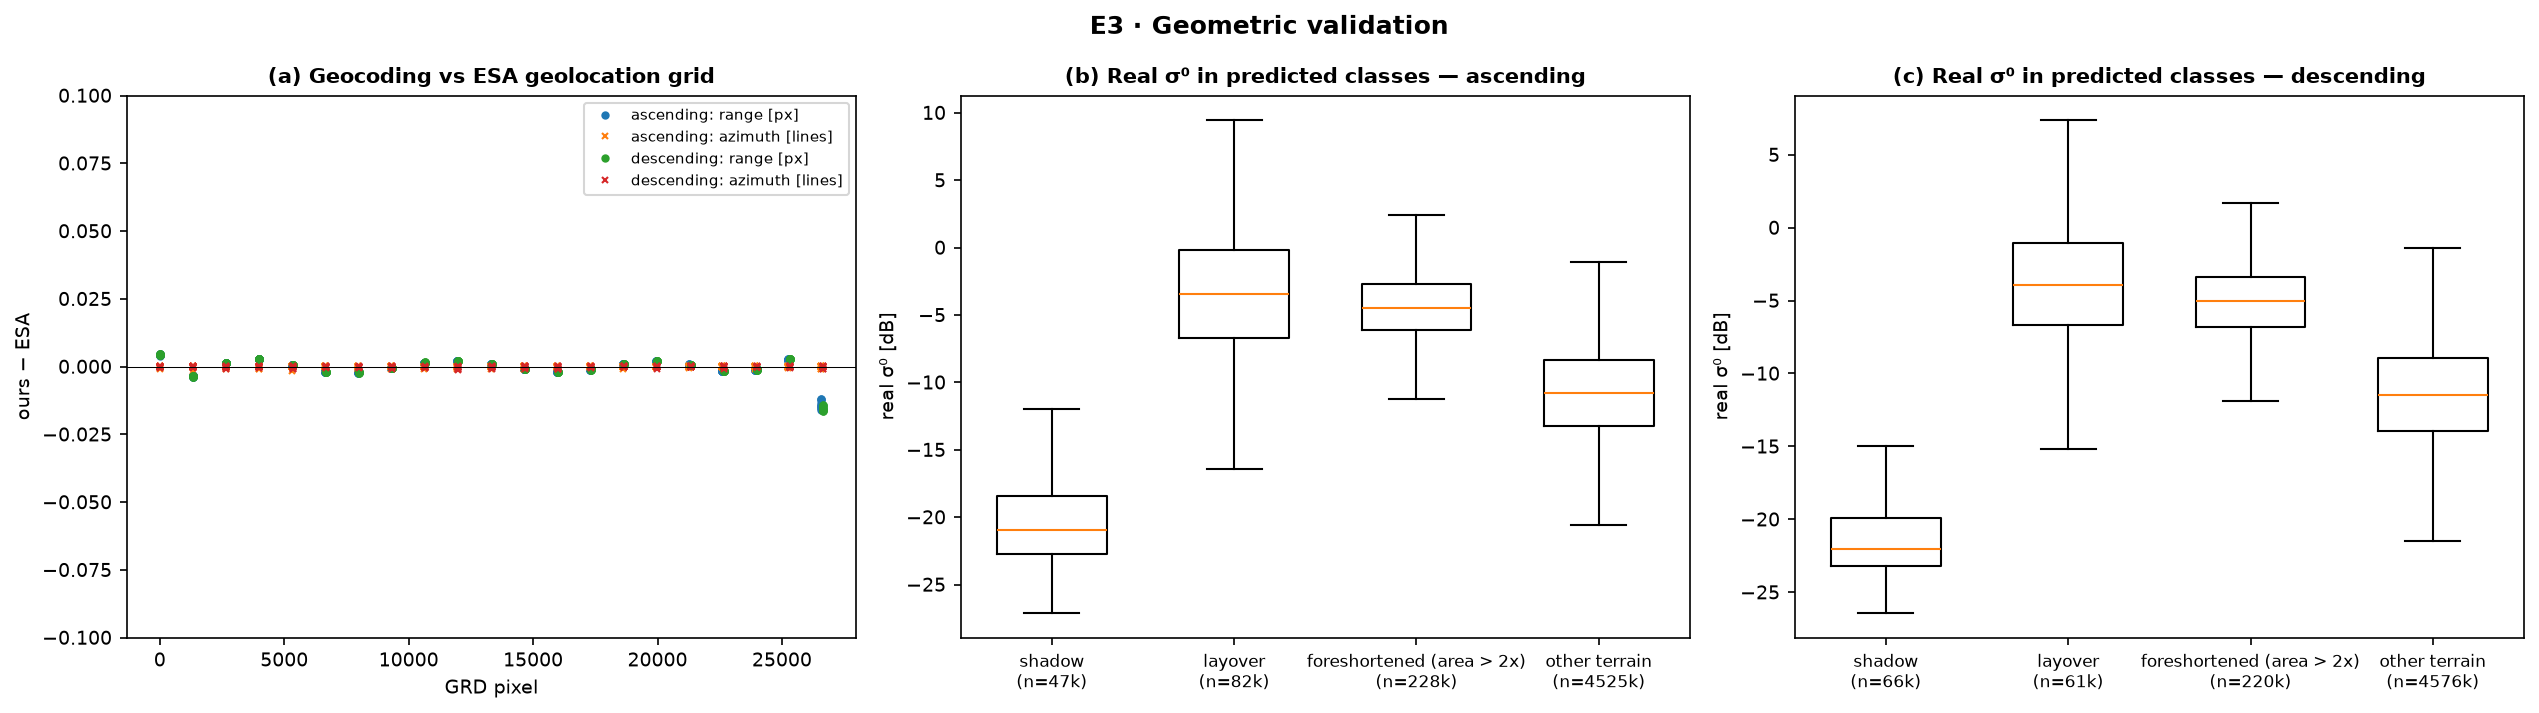
\includegraphics[width=\textwidth]{p4_geometric_validation.png}
\caption[Geometric validation]{Geometric validation: (\textbf{a}) geocoding residuals with respect to the geolocation grid of both products; (\textbf{b},\textbf{c}) real $\sigz$ in the predicted classes for the ascending and descending scenes.}
\label{fig:geomval}
\end{figure}

\section{Sensitivity to Processing Choices}
Table~\ref{tab:sens} and Fig.~\ref{fig:sens} vary one processing choice at a time. Omitting the geoid correction ($N=\geoidN$\,m) moves the simulation by 5.8 pixels (58\,m) in range, in agreement with the expected ground-range displacement $N/\tan\theta$ of about 61\,m of a height error $N$ at an incidence angle of about 39$^\circ$; co-registration absorbs this shift and the correlation is unchanged, but an un-co-registered product such as a layover and shadow mask would be misplaced by six pixels. Without DEM oversampling, \holesNoOver\,\% of the GRD pixels receive no facet, compared with \holesBase\,\% with threefold oversampling, in a striped pattern on all slopes facing away from the radar. After $5\times5$ multilooking the correlation hardly changes ($r=\rNoOver$), but single-look products and masks would be unusable. A 90\,m DEM gives the same correlation as GLO-30 ($r=\rDemNinety$): at the 50\,m scale of the comparison, the large landforms dominate, and the finer DEM matters for full-resolution products.

\begin{table}[htbp]
\caption[Sensitivity of the simulation (ascending scene, fitted law)]{Sensitivity of the simulation (ascending scene, fitted law). $\Delta$line and $\Delta$pixel are the residual shifts found by co-registration.}
\label{tab:sens}
\centering\small
\resizebox{\textwidth}{!}{\begin{tabular}{lrrrrr}\toprule
 Configuration & $r$ & SSIM & $\Delta$line & $\Delta$pixel & empty px [\%]\\\midrule
baseline (GLO-30, 3x oversampled, geoid) & 0.710 & 0.508 & -2.2 & 3.5 & 0.01 \\
no geoid correction (N = 0) & 0.710 & 0.507 & -2.2 & -2.3 & 0.01 \\
no DEM oversampling & 0.706 & 0.446 & -2.2 & 3.5 & 45.82 \\
90 m DEM (GLO-30 aggregated 3x3) & 0.714 & 0.418 & -2.3 & 3.5 & 0.00 \\
\bottomrule\end{tabular}
}
\end{table}
\begin{figure}[htbp]
\centering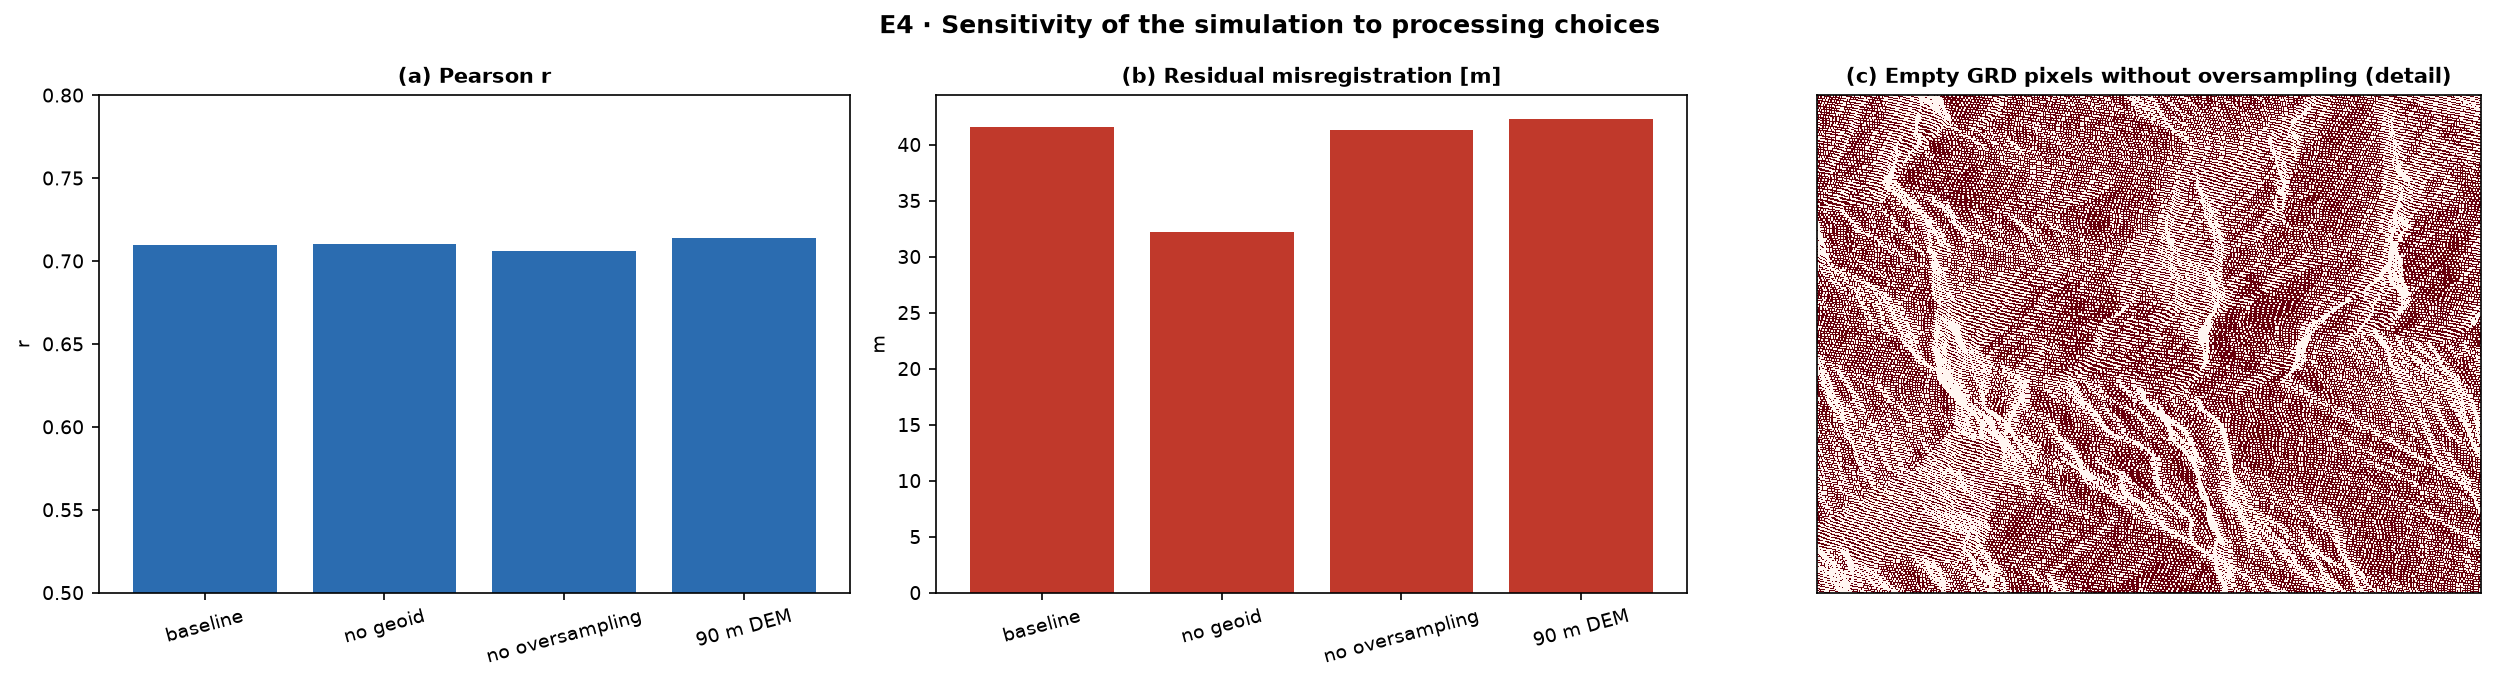
\includegraphics[width=\textwidth]{p5_sensitivity.png}
\caption[Sensitivity]{Sensitivity: (\textbf{a}) correlation; (\textbf{b}) residual misregistration; (\textbf{c}) GRD pixels that receive no facet without DEM oversampling (detail of the Nordkette).}
\label{fig:sens}
\end{figure}

\section{Contribution of Land Cover}
Grouping the residuals by WorldCover class (Table~\ref{tab:lc}, Figs.~\ref{fig:lc} and~\ref{fig:resmap}) shows where a DEM-only simulation fails. Tree cover, which represents 55\,\% of the area, is reproduced without bias ($-0.1$\,dB) and with the highest correlation ($r=0.86$): the volume scattering of the forest canopy is close to the smooth angular law fitted to a scene that forest dominates. Built-up areas ($+3.1$\,dB) are brighter than predicted because double-bounce reflections between walls and the ground are absent from any facet model~\cite{balz2009,auer2010}; bare rock and scree ($+3.2$\,dB) are rougher than the average surface. Water ($-3.8$\,dB), cropland ($-2.0$\,dB) and grassland ($-1.4$\,dB) are darker because smooth surfaces reflect specularly away from the radar~\cite{ulaby1982}. The low correlations within the built-up, cropland and water classes ($r=0.22$--$0.30$) do not indicate a geometric failure: these classes lie on the flat valley floor, where the DEM predicts an almost constant value and the terrain signal to correlate with is weak.

\begin{table}[htbp]
\caption[Residual (real minus simulated $\sigz$) and correlation per land-cover class (ascending scene, map geometry, layover and shadow excluded)]{Residual (real minus simulated $\sigz$) and correlation per land-cover class (ascending scene, map geometry, layover and shadow excluded).}
\label{tab:lc}
\centering\small
\begin{tabular}{lrrrr}\toprule
 WorldCover class & area [\%] & mean residual [dB] & std [dB] & $r$\\\midrule
Tree cover & 55.3 & -0.14 & 2.52 & 0.86 \\
Grassland & 25.9 & -1.44 & 3.28 & 0.77 \\
Cropland & 3.9 & -2.00 & 2.54 & 0.23 \\
Built-up & 7.2 & 3.11 & 4.54 & 0.22 \\
Bare / sparse & 5.8 & 3.18 & 4.29 & 0.82 \\
Snow \& ice & 0.3 & 2.09 & 2.91 & 0.86 \\
Water & 0.5 & -3.76 & 4.12 & 0.30 \\
Moss \& lichen & 1.2 & 0.51 & 3.27 & 0.88 \\
\bottomrule\end{tabular}

\end{table}
\begin{figure}[htbp]
\centering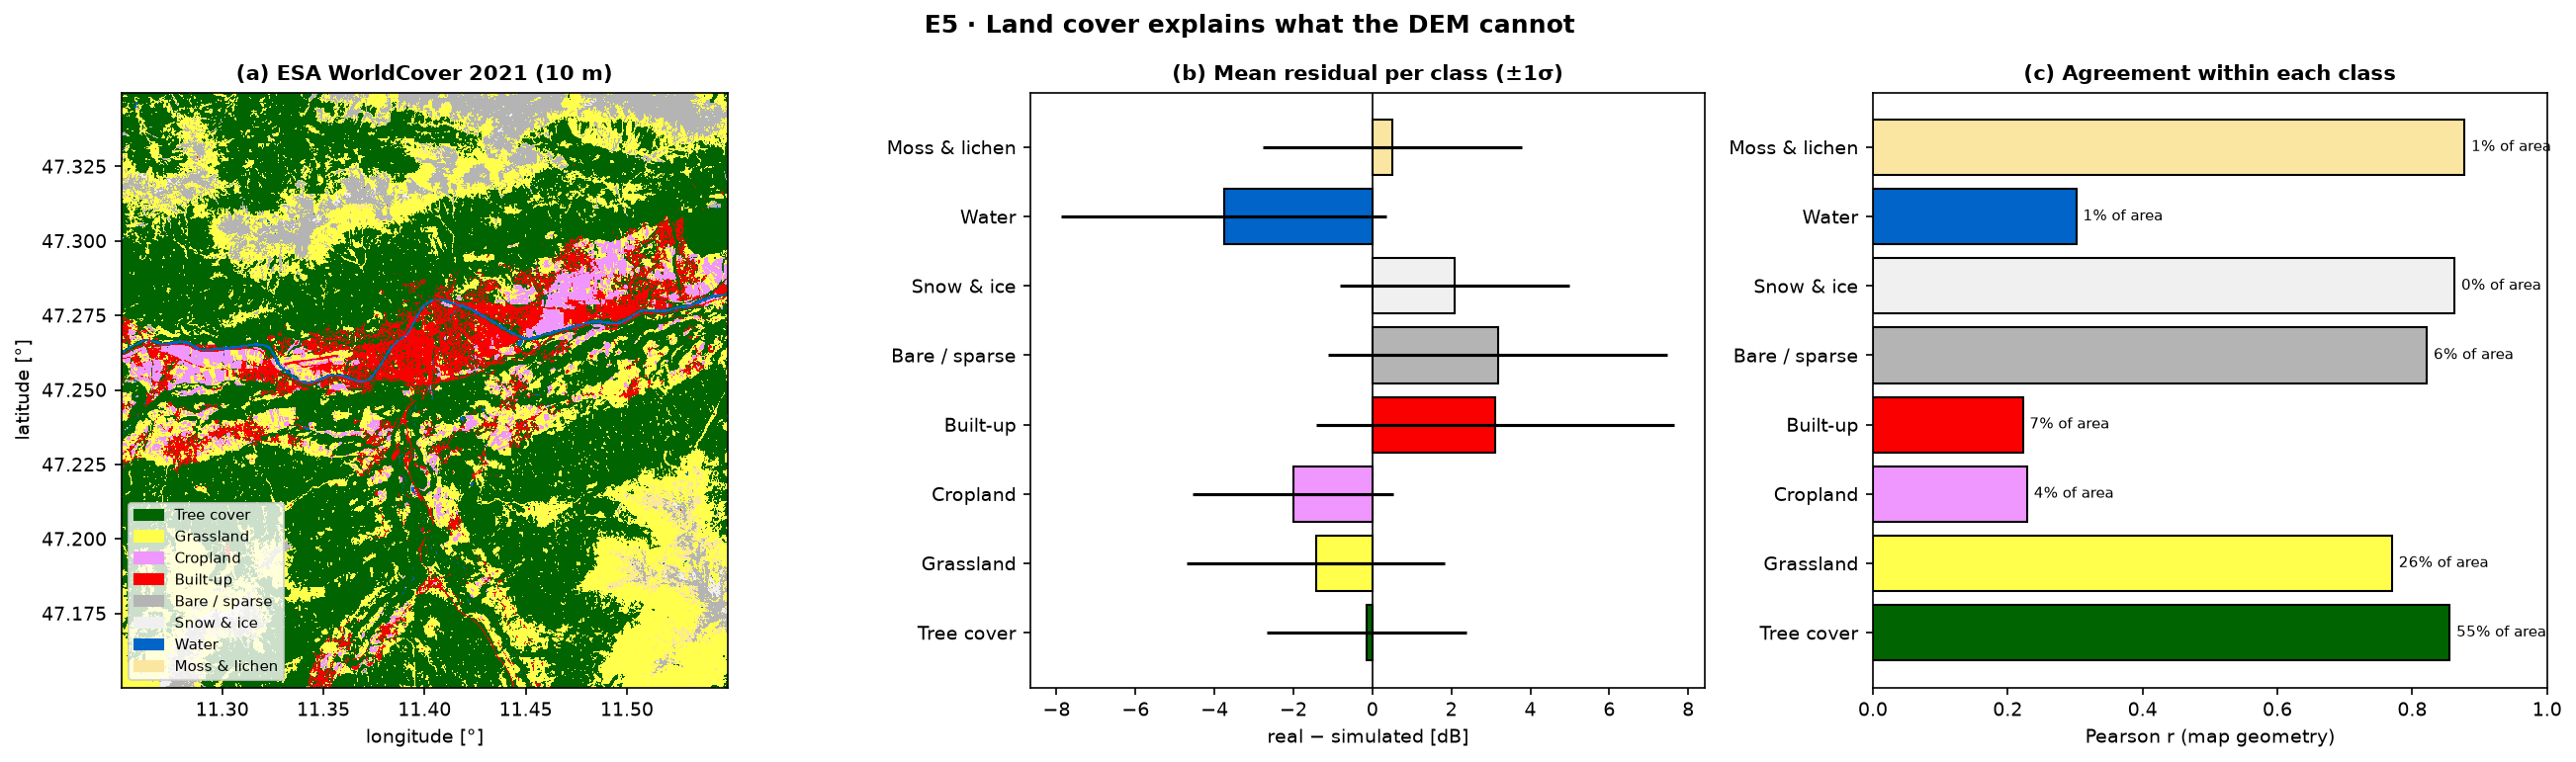
\includegraphics[width=\textwidth]{p6_landcover.png}
\caption[Land cover]{Land cover: (\textbf{a}) ESA WorldCover map of the study site; (\textbf{b}) mean residual per class ($\pm1$ standard deviation); (\textbf{c}) correlation within each class.}
\label{fig:lc}
\end{figure}
\begin{figure}[htbp]
\centering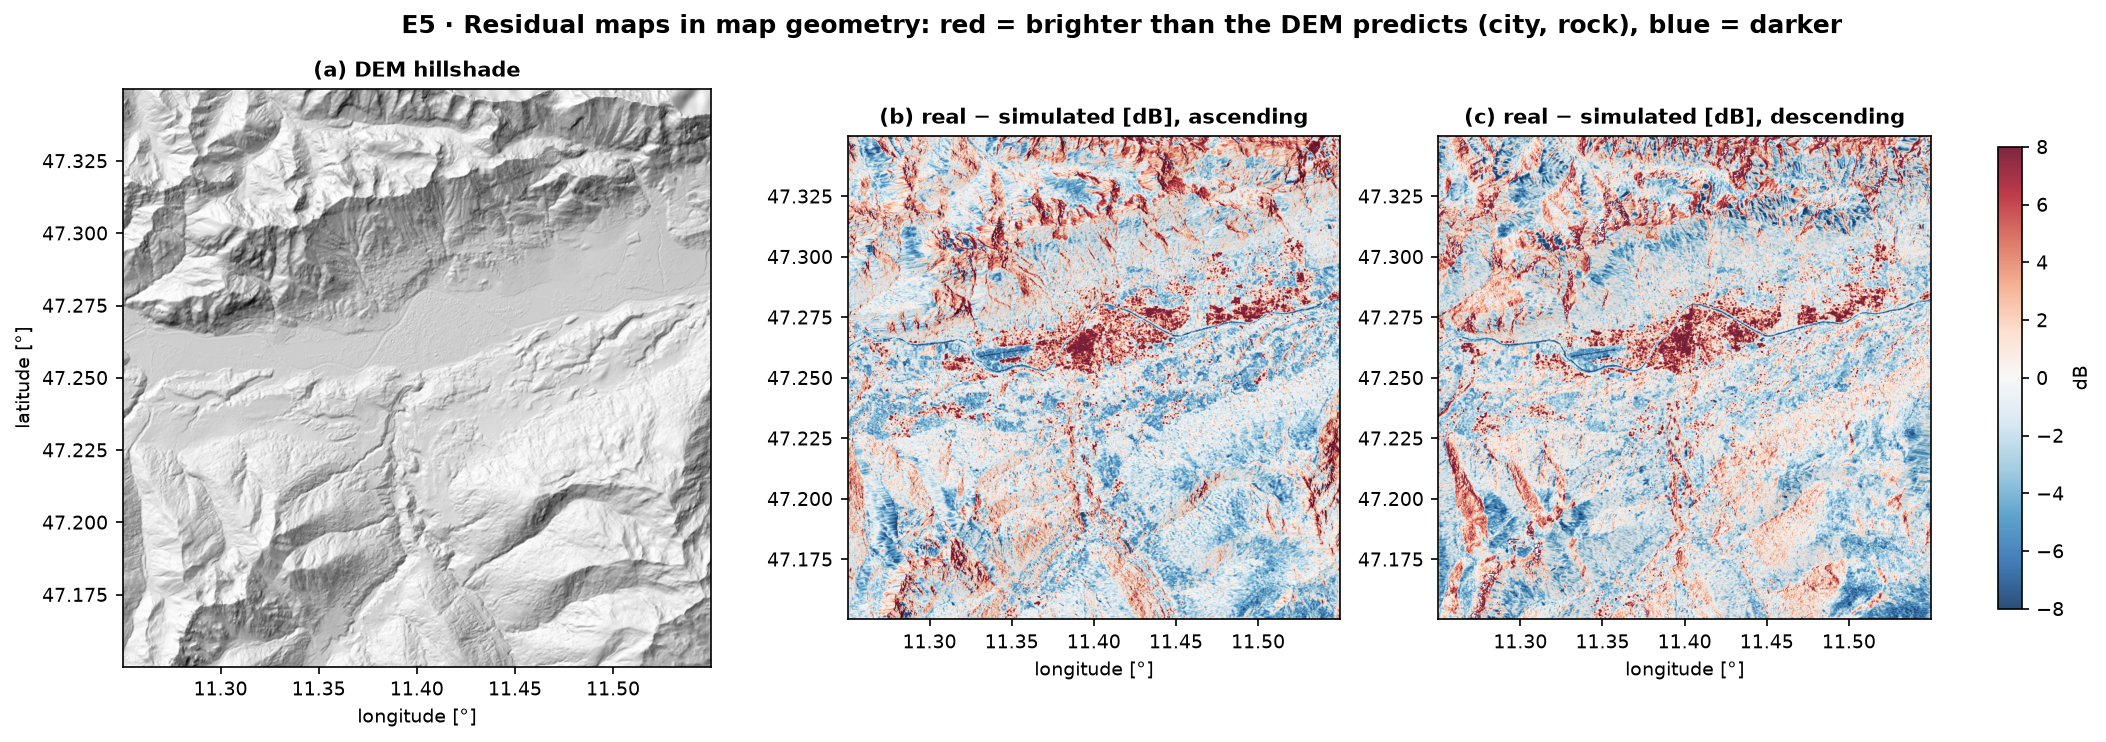
\includegraphics[width=\textwidth]{p7_residual_maps.png}
\caption[DEM hillshade and residual maps (real minus simulated $\sigz$) in map geometry for the ascending and descending scenes]{DEM hillshade (\textbf{a}) and residual maps (real minus simulated $\sigz$) in map geometry for the ascending (\textbf{b}) and descending (\textbf{c}) scenes.}
\label{fig:resmap}
\end{figure}

\section{Limitations of the Study}
The results presented in this section show that terrain geometry explains a large part of Sentinel-1 images of Alpine terrain. A few limitations related to the data and the methodology should nevertheless be discussed.

First, co-registration still finds offsets between image and simulation of \shiftAscL{} lines and \shiftAscP{} pixels (about 22\,m in azimuth and 35\,m in range) for the ascending scene and \shiftDescL{} lines and \shiftDescP{} pixels for the descending scene. Because the geocoding reproduces the product annotation to a small fraction of a pixel, these offsets measure the discrepancy between the image content and the annotated geolocation of the products, combined with DEM errors on steep slopes. Atmospheric path delay, solid-earth tides and the orbit used for near-real-time products, which are not modelled here, are known to contribute to the absolute geolocation error of Sentinel-1~\cite{schubert2015,gisinger2021}. Such offsets are routinely removed by simulation-based co-registration~\cite{nitti2011,small2011}.

Second, the simulator is an incoherent single-bounce model. It does not represent double bounce, volume scattering or multipath, which explains the residuals over built-up areas and the spread of real $\sigz$ at a given local incidence angle. Third, thermal noise was not removed, so that predicted shadow is compared with the noise floor rather than with zero. Fourth, one date per geometry was used; seasonal effects such as snow cover or soil moisture, and the time difference between the DEM acquisitions and the 2025 images, were not analysed. Finally, the absolute level of each backscatter law was calibrated by a constant; absolute radiometric prediction would require a land-cover-dependent model. These limitations do not affect the geometric conclusions of this study.

\chapter{Software Implementation}
\label{ch:software}
The methodology of Chapter~\ref{ch:method} is implemented as an open Python package, an experiment pipeline, a
tutorial notebook and a graphical application. This chapter describes their structure and use. All components run in a
single environment pinned with the \texttt{uv} package manager (Python 3.12), and all input data are streamed from the
Microsoft Planetary Computer without registration and cached locally \cite{planetary}.

\section{Software Architecture}
The package \texttt{sarsim} contains five modules, each responsible for one stage of the data flow of
Fig.~\ref{fig:dataflow}. The module \texttt{data} provides cached access to the Copernicus GLO-30 DEM, to the window of
a Sentinel-1 GRD product that covers the DEM together with its annotation and calibration files, and to the ESA
WorldCover map. The module \texttt{s1} parses the product annotation, fits the orbit polynomial, solves the
zero-Doppler condition, applies the piece-wise slant-to-ground-range conversion and calibrates digital numbers to
$\sigma^0$. The module \texttt{rdsim} computes the facet geometry block-wise, flags shadow and layover, evaluates the
backscatter laws and renders the simulated image by bilinear splatting. The module \texttt{compare} implements
multilooking, sub-pixel co-registration, the similarity metrics and back-geocoding to the DEM grid. The module
\texttt{geodesy}, finally, provides the conversions between geodetic and Earth-centred coordinates and the EGM2008
geoid undulation. The repository structure is listed in Appendix~\ref{app:structure}.

\section{Experiment Pipeline}
The script \texttt{run\_all.py} carries out experiments E1 to E5 of Section~\ref{sec:final-design} and
Chapter~\ref{ch:method} in one run: it downloads and caches the data, computes the facet geometry once per scene,
renders the five backscatter laws, evaluates both viewing geometries, repeats the simulation for the sensitivity
cases and analyses the residuals per land-cover class. All numbers are written to \texttt{results/metrics.json} and to
CSV tables, and all figures of Chapter~\ref{ch:results} that are prefixed with ``E'' are written to
\texttt{figures/pipeline/}. The tables and numbers quoted in this report are generated from \texttt{metrics.json} by
the script \texttt{report/make\_tables.py}, so that the text cannot drift from the results. A complete run takes about
fifteen minutes on a laptop with 16\,GB of memory.

\section{Verification and Testing}
Eight unit tests guard the geometric core of the simulator. They check that flat terrain produces neither shadow nor
layover, that steep fore-slopes and back-slopes are classified as layover and shadow, that gentle slopes are
classified as neither, that the backscatter laws decrease monotonically, that the bilinear splatting conserves energy,
that the geodetic conversion is exact at the equator and the pole, that the block-wise facet geometry does not depend on
the block size, and that the range-Doppler geocoding reproduces the zero-Doppler times and pixel positions of the
geolocation grid of a real Sentinel-1 product. All tests pass.

\section{Tutorial Notebook}
The notebook \texttt{notebooks/01\_sar\_simulation\_walkthrough.ipynb} reproduces the verification sequence of
Section~\ref{sec:res-verif} step by step: a single point target and pulse, a line of targets, the moving satellite with
raw, range-compressed and focused data, a flat surface with speckle, a sinusoidal surface, a real DEM patch, the
geometric distortions, the radiometric chain and, finally, the comparison with a real Sentinel-1 scene. Each step is
shown as a sequence of plots that follows the processing chain, which makes the notebook usable as teaching material.

\section{Graphical Application}
\label{sec:gui}
To make the simulator usable without programming, a graphical application was developed with the Streamlit framework.
It runs the complete simulation for a DEM of any location and returns the simulated SAR data in formats suitable for
research use. As illustrated in Fig.~\ref{fig:gui-start}, all inputs are grouped in a sidebar and a single
\emph{Run simulation} button starts the processing, while the main area is divided into an \emph{Overview} and a
\emph{Results} tab. An information button in the top-right corner opens a panel that explains how to use the
application and how the simulation works (Fig.~\ref{fig:gui-info}).

The terrain can be selected from presets, defined by a bounding box, in which case the Copernicus GLO-30 DEM is
downloaded and cached, or uploaded as a GeoTIFF in any projection, which is reprojected to geographic coordinates.
Two geometry modes are offered. The generic mode simulates a Sentinel-1-like sensor on a straight orbit at 693\,km over
a flat Earth for any location and works offline once the DEM is available; the user chooses the pass (ascending,
looking east, or descending, looking west), the look angle and, optionally, the heading, the pixel spacing and the
orbit height. The real mode searches the Sentinel-1 catalogue for a scene covering the area, simulates in the exact
geometry of that product with the methodology of Chapter~\ref{ch:method}, and compares the simulation with the real
image using the metrics of Section~\ref{sec:res-verif} and Chapter~\ref{ch:results}. The backscatter law is selected
among the five laws of Table~\ref{tab:models}, with the fitted law as the default, and speckle and multilooking can be
added. A memory guard limits the number of facets by reducing the oversampling and, if necessary, aggregating the DEM,
and reports when it does so.

After a run, the Overview tab summarises the area, the DEM grid, the height range, the fractions of layover and
shadow and the run time, together with a hillshade of the terrain and the configuration used
(Fig.~\ref{fig:gui-overview}). The Results tab shows the simulated $\sigma^0$ in radar and in map geometry, the layover
and shadow masks, the local incidence angle with its histogram and the $\sigma^0$ curve against the local incidence
angle, and, in the real mode, the real and simulated images side by side with a density scatter plot and the
agreement metrics (Fig.~\ref{fig:gui-results}). A download button provides a ZIP archive that contains map-geometry
GeoTIFFs of the simulated $\sigma^0$ (linear and in dB), the local incidence angle, the layover and shadow masks and the
DEM used, the radar-geometry image as GeoTIFF and NumPy array, and a metadata file that records all inputs, sensor
parameters and the software version. The full Innsbruck scene is simulated in about 10\,s in the generic mode and
about 35\,s in the real mode, and the application is covered by headless tests that run the complete pipeline from the
\emph{Run simulation} button.

\begin{figure}[htbp]
\centering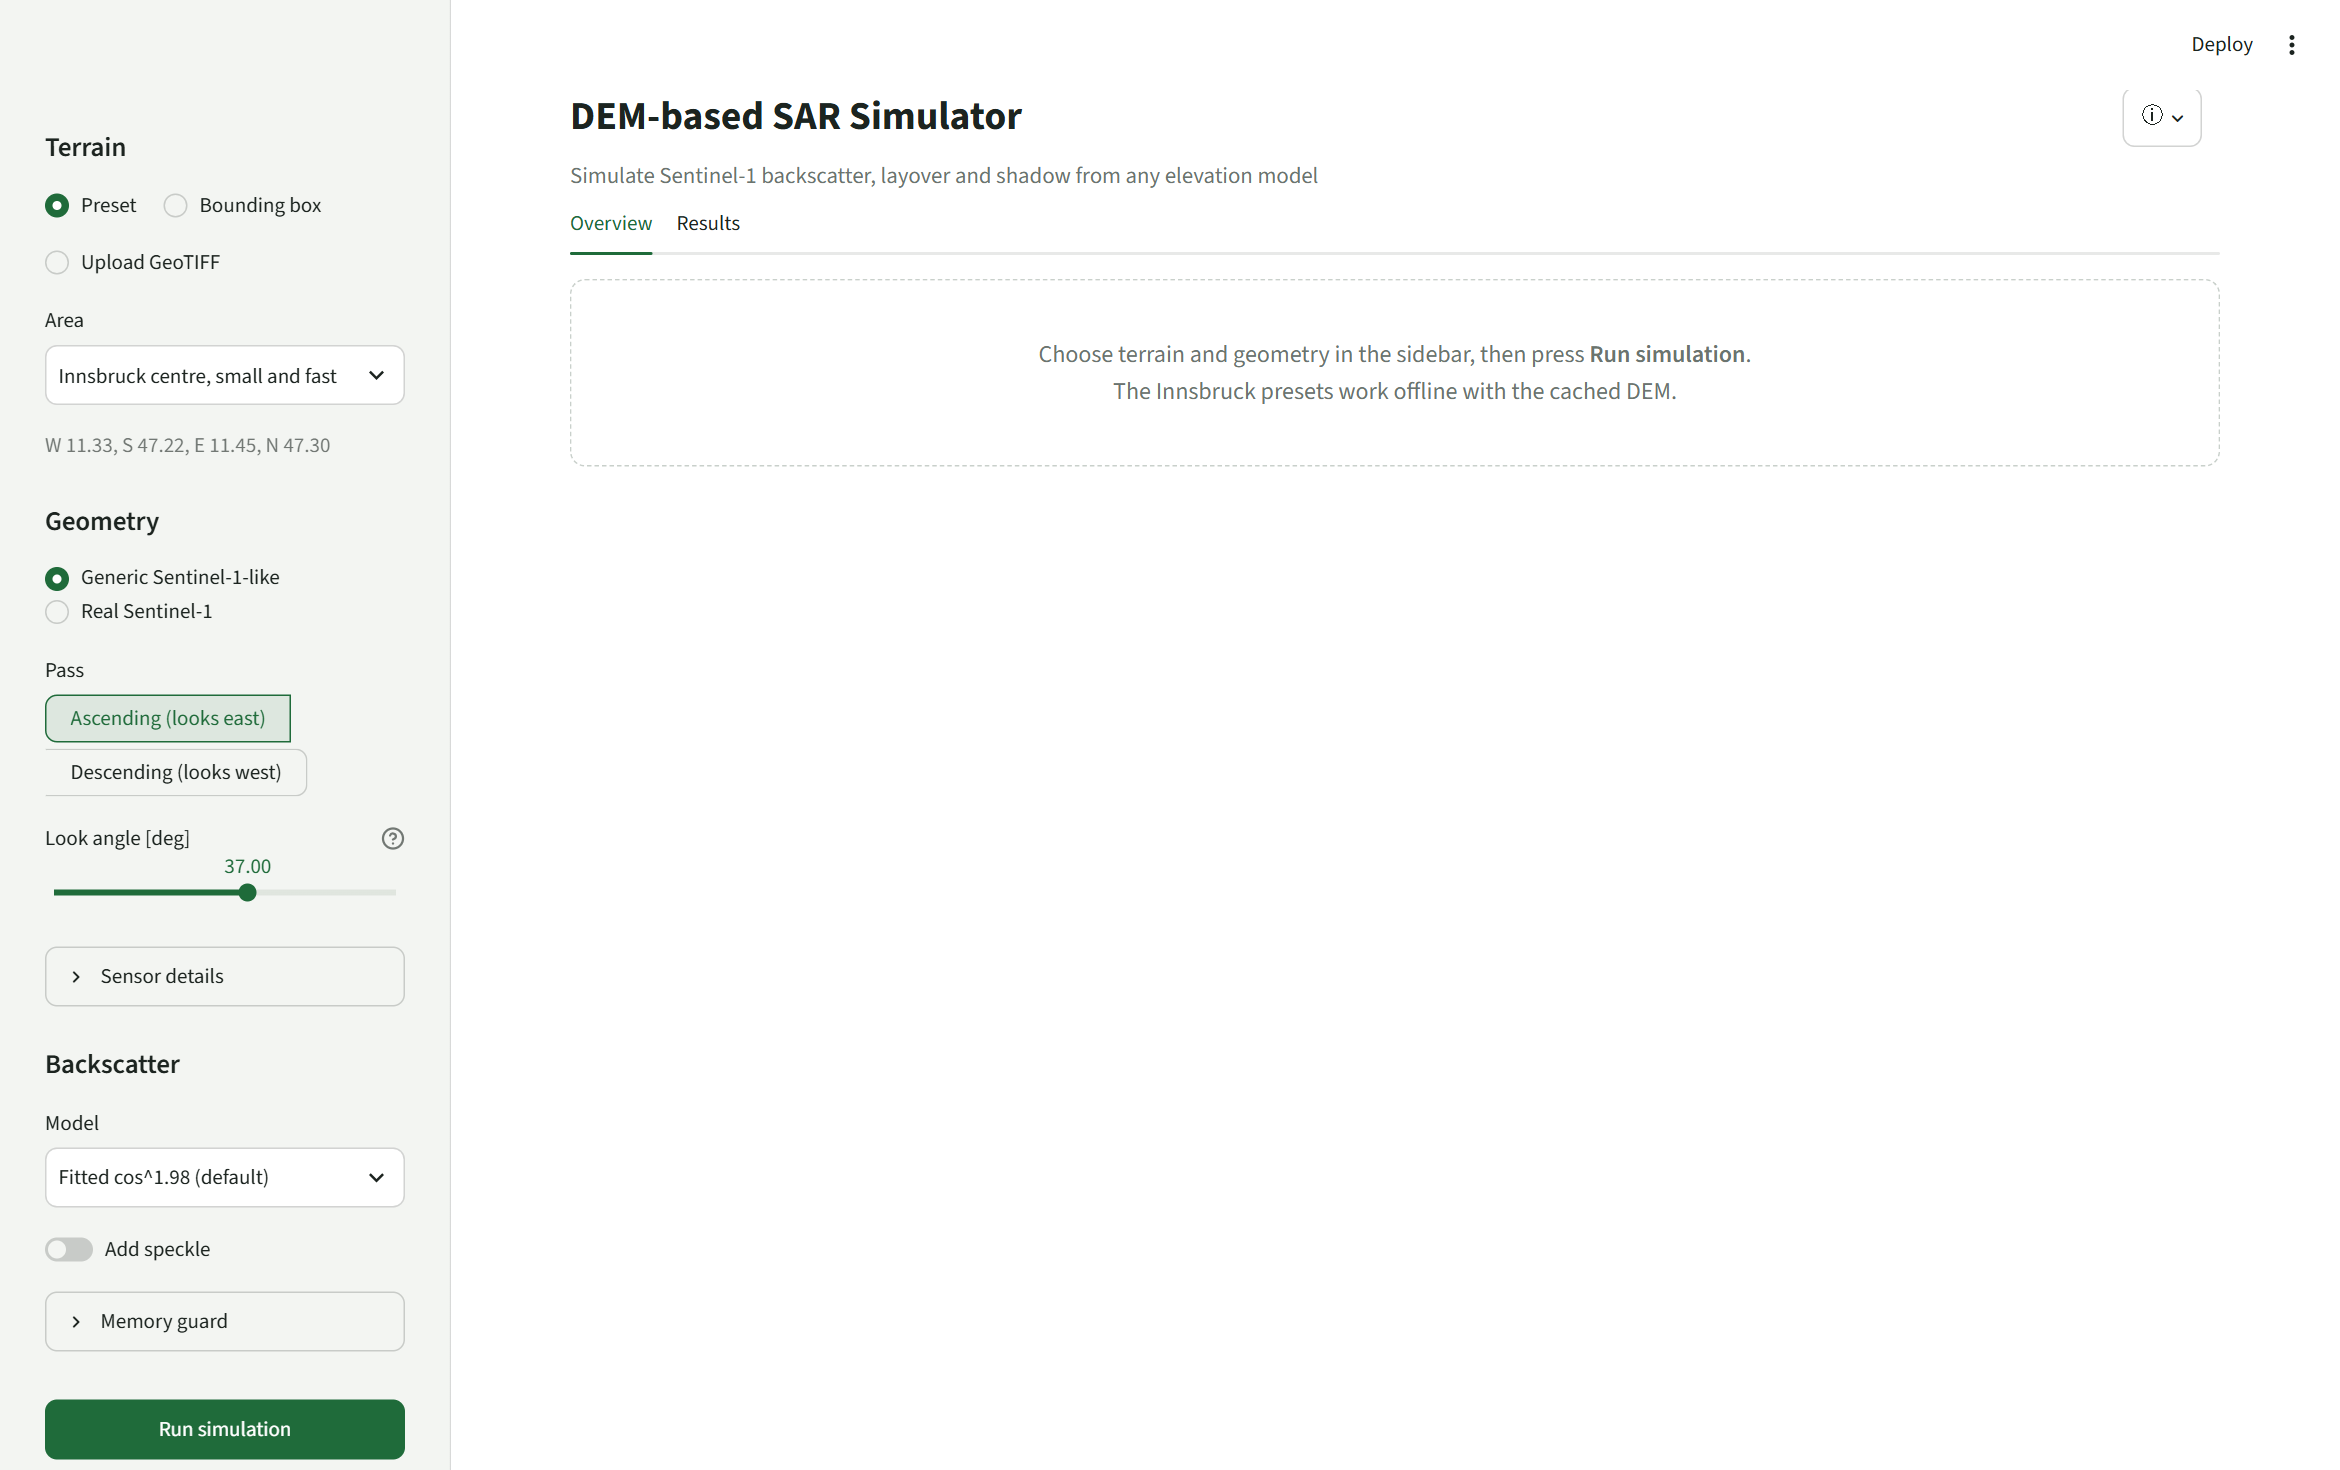
\includegraphics[width=\textwidth]{gui_01_start.png}
\caption[Graphical application: start page]{Graphical application: start page with the input sidebar (terrain,
geometry, backscatter, memory guard) and the information button in the top-right corner.}
\label{fig:gui-start}
\end{figure}
\begin{figure}[htbp]
\centering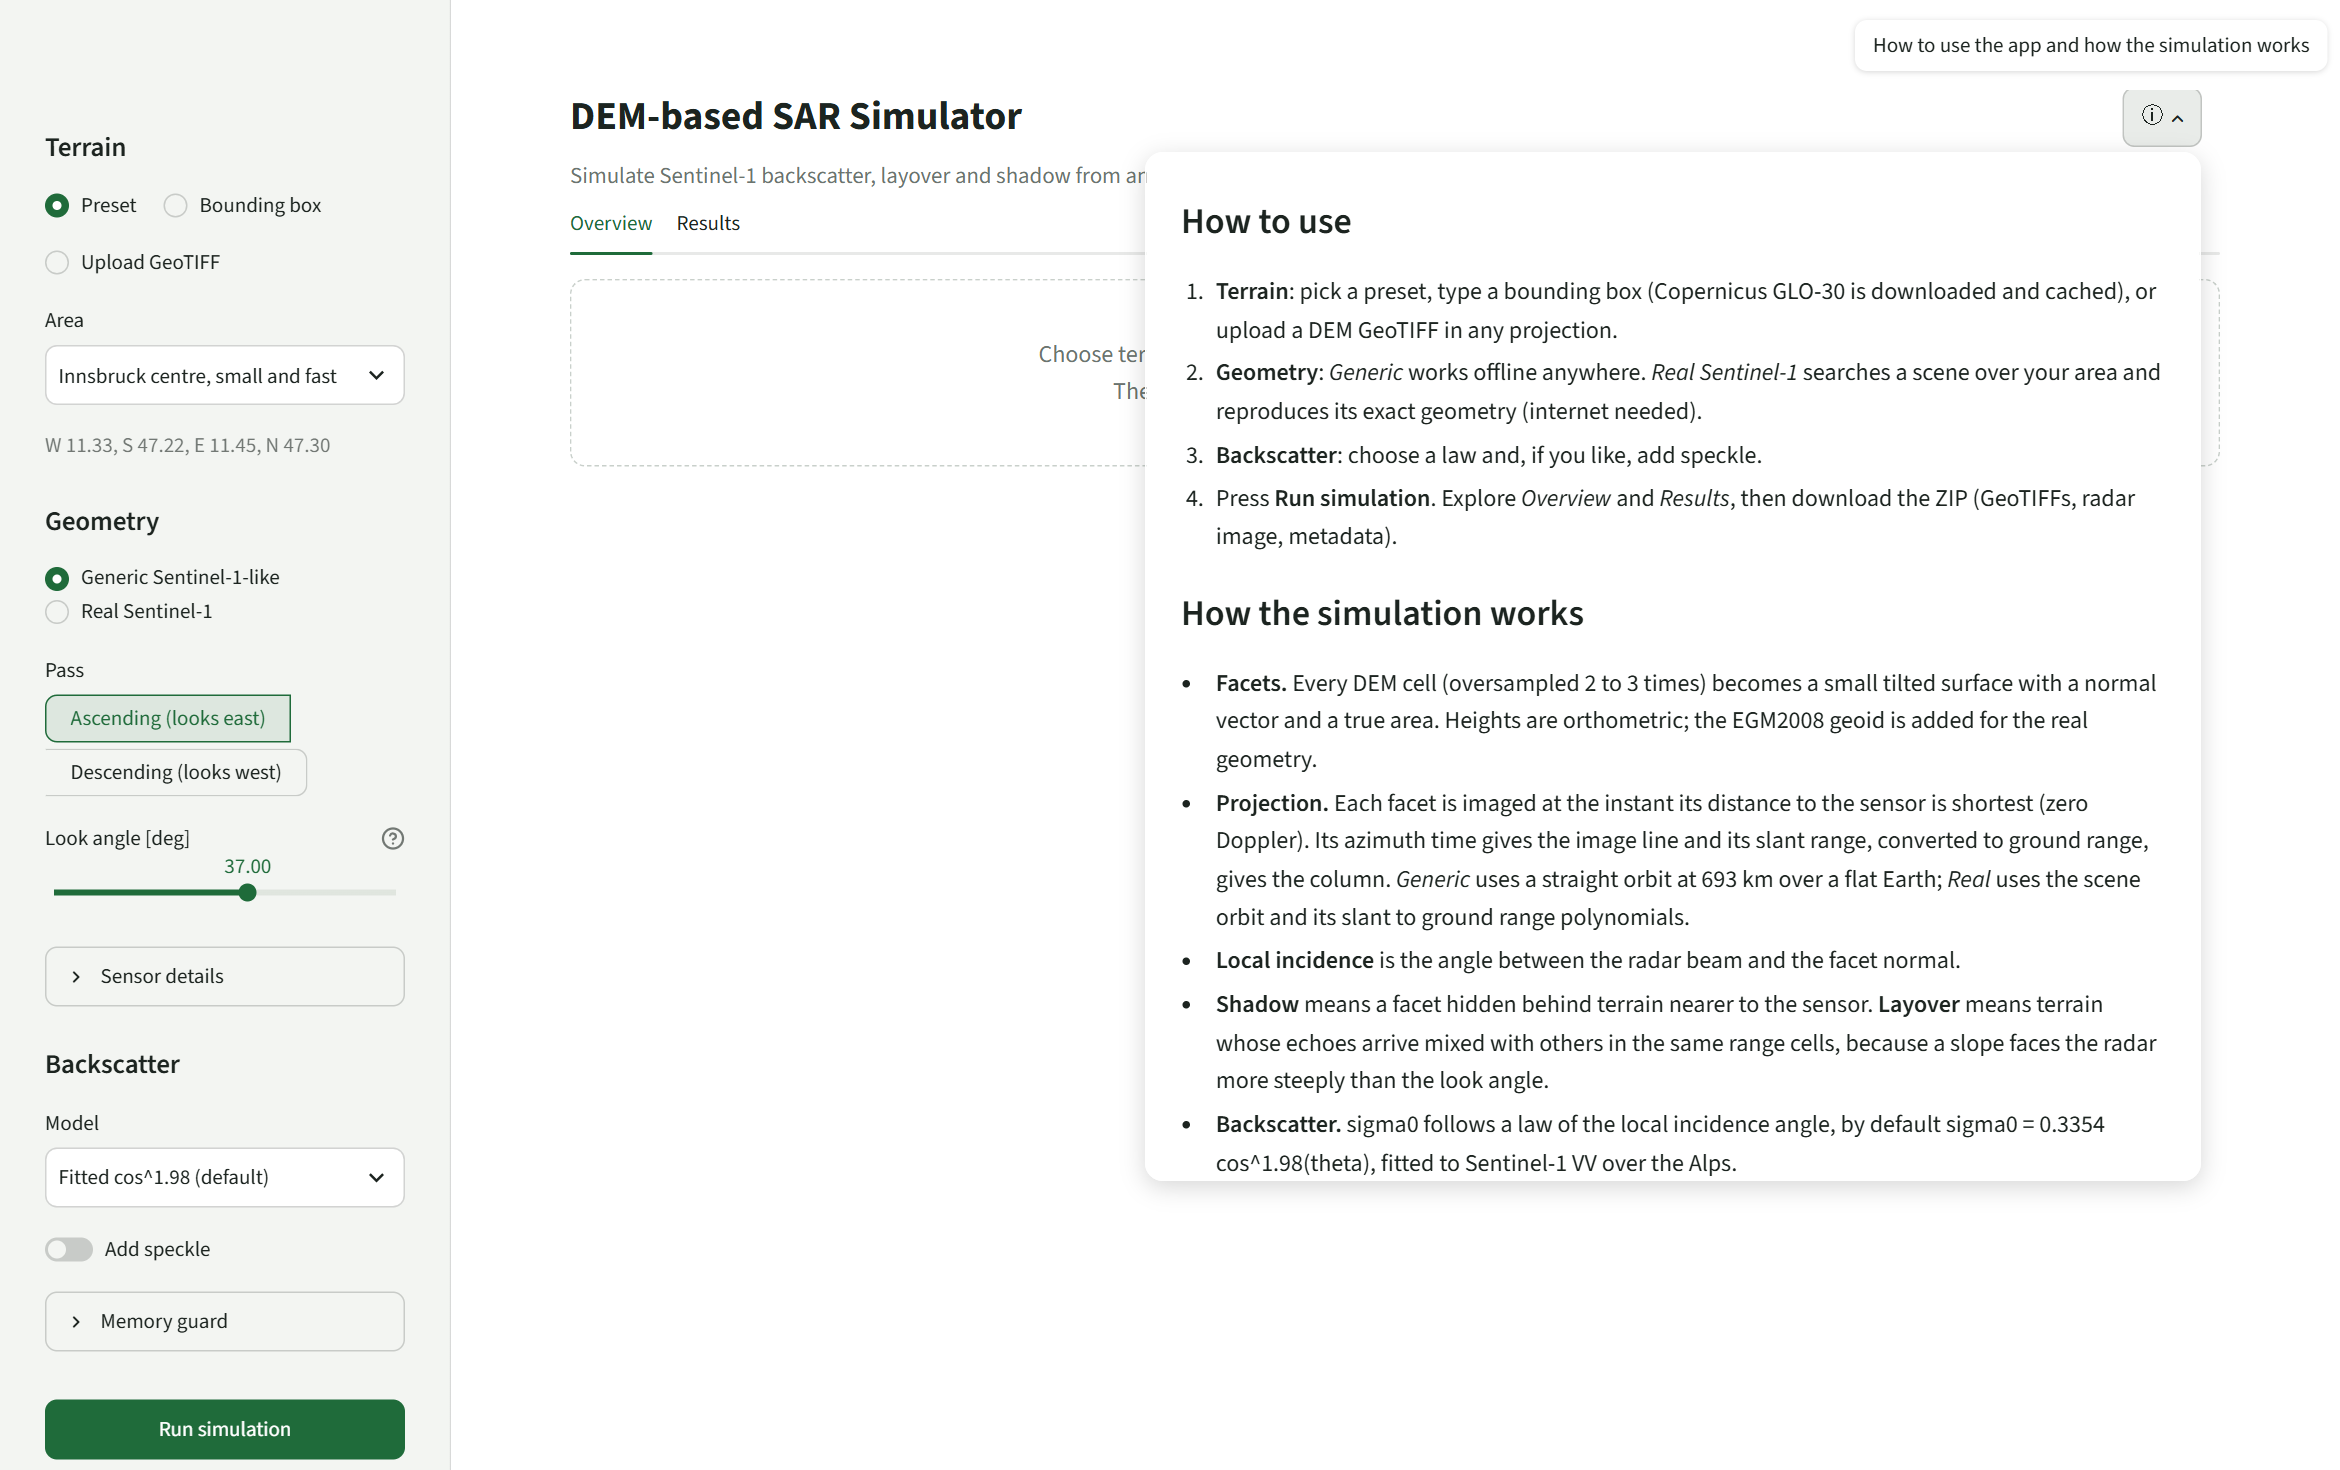
\includegraphics[width=\textwidth]{gui_02_info.png}
\caption[Graphical application: information panel]{Graphical application: information panel explaining how to use the
application and how the simulation works.}
\label{fig:gui-info}
\end{figure}
\begin{figure}[htbp]
\centering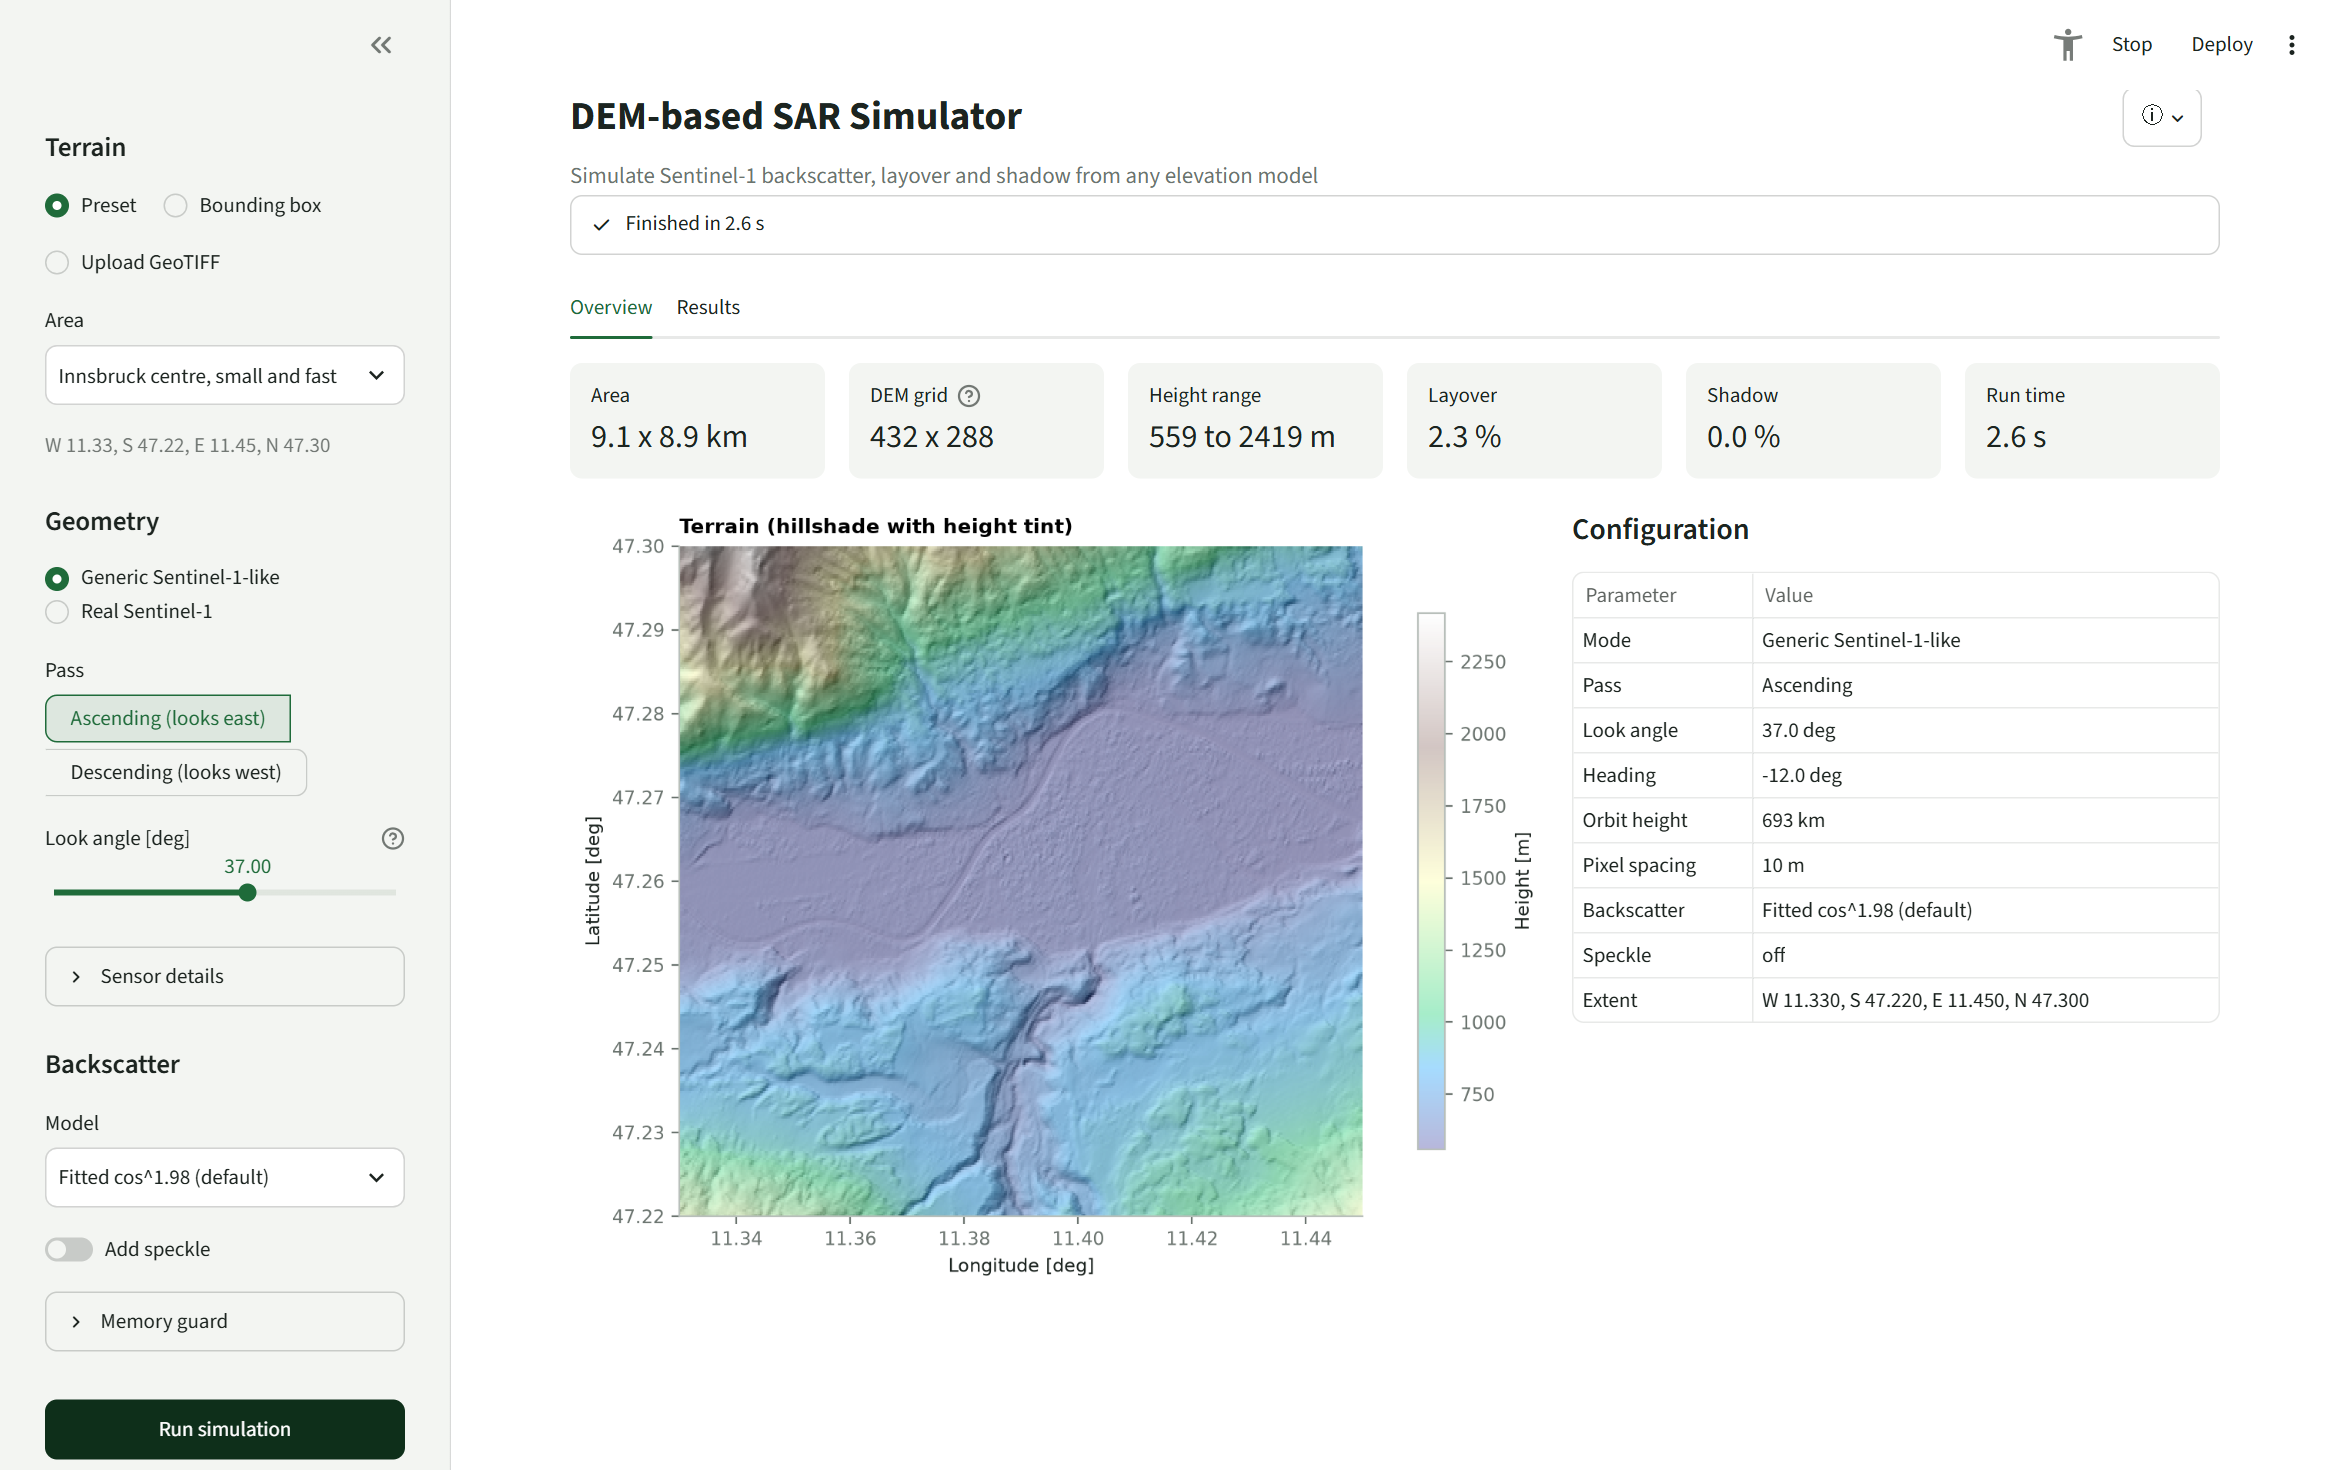
\includegraphics[width=\textwidth]{gui_03_overview.png}
\caption[Graphical application: Overview tab]{Graphical application: Overview tab after a run in the generic mode
over the Innsbruck preset, with summary cards, terrain hillshade and configuration.}
\label{fig:gui-overview}
\end{figure}
\begin{figure}[htbp]
\centering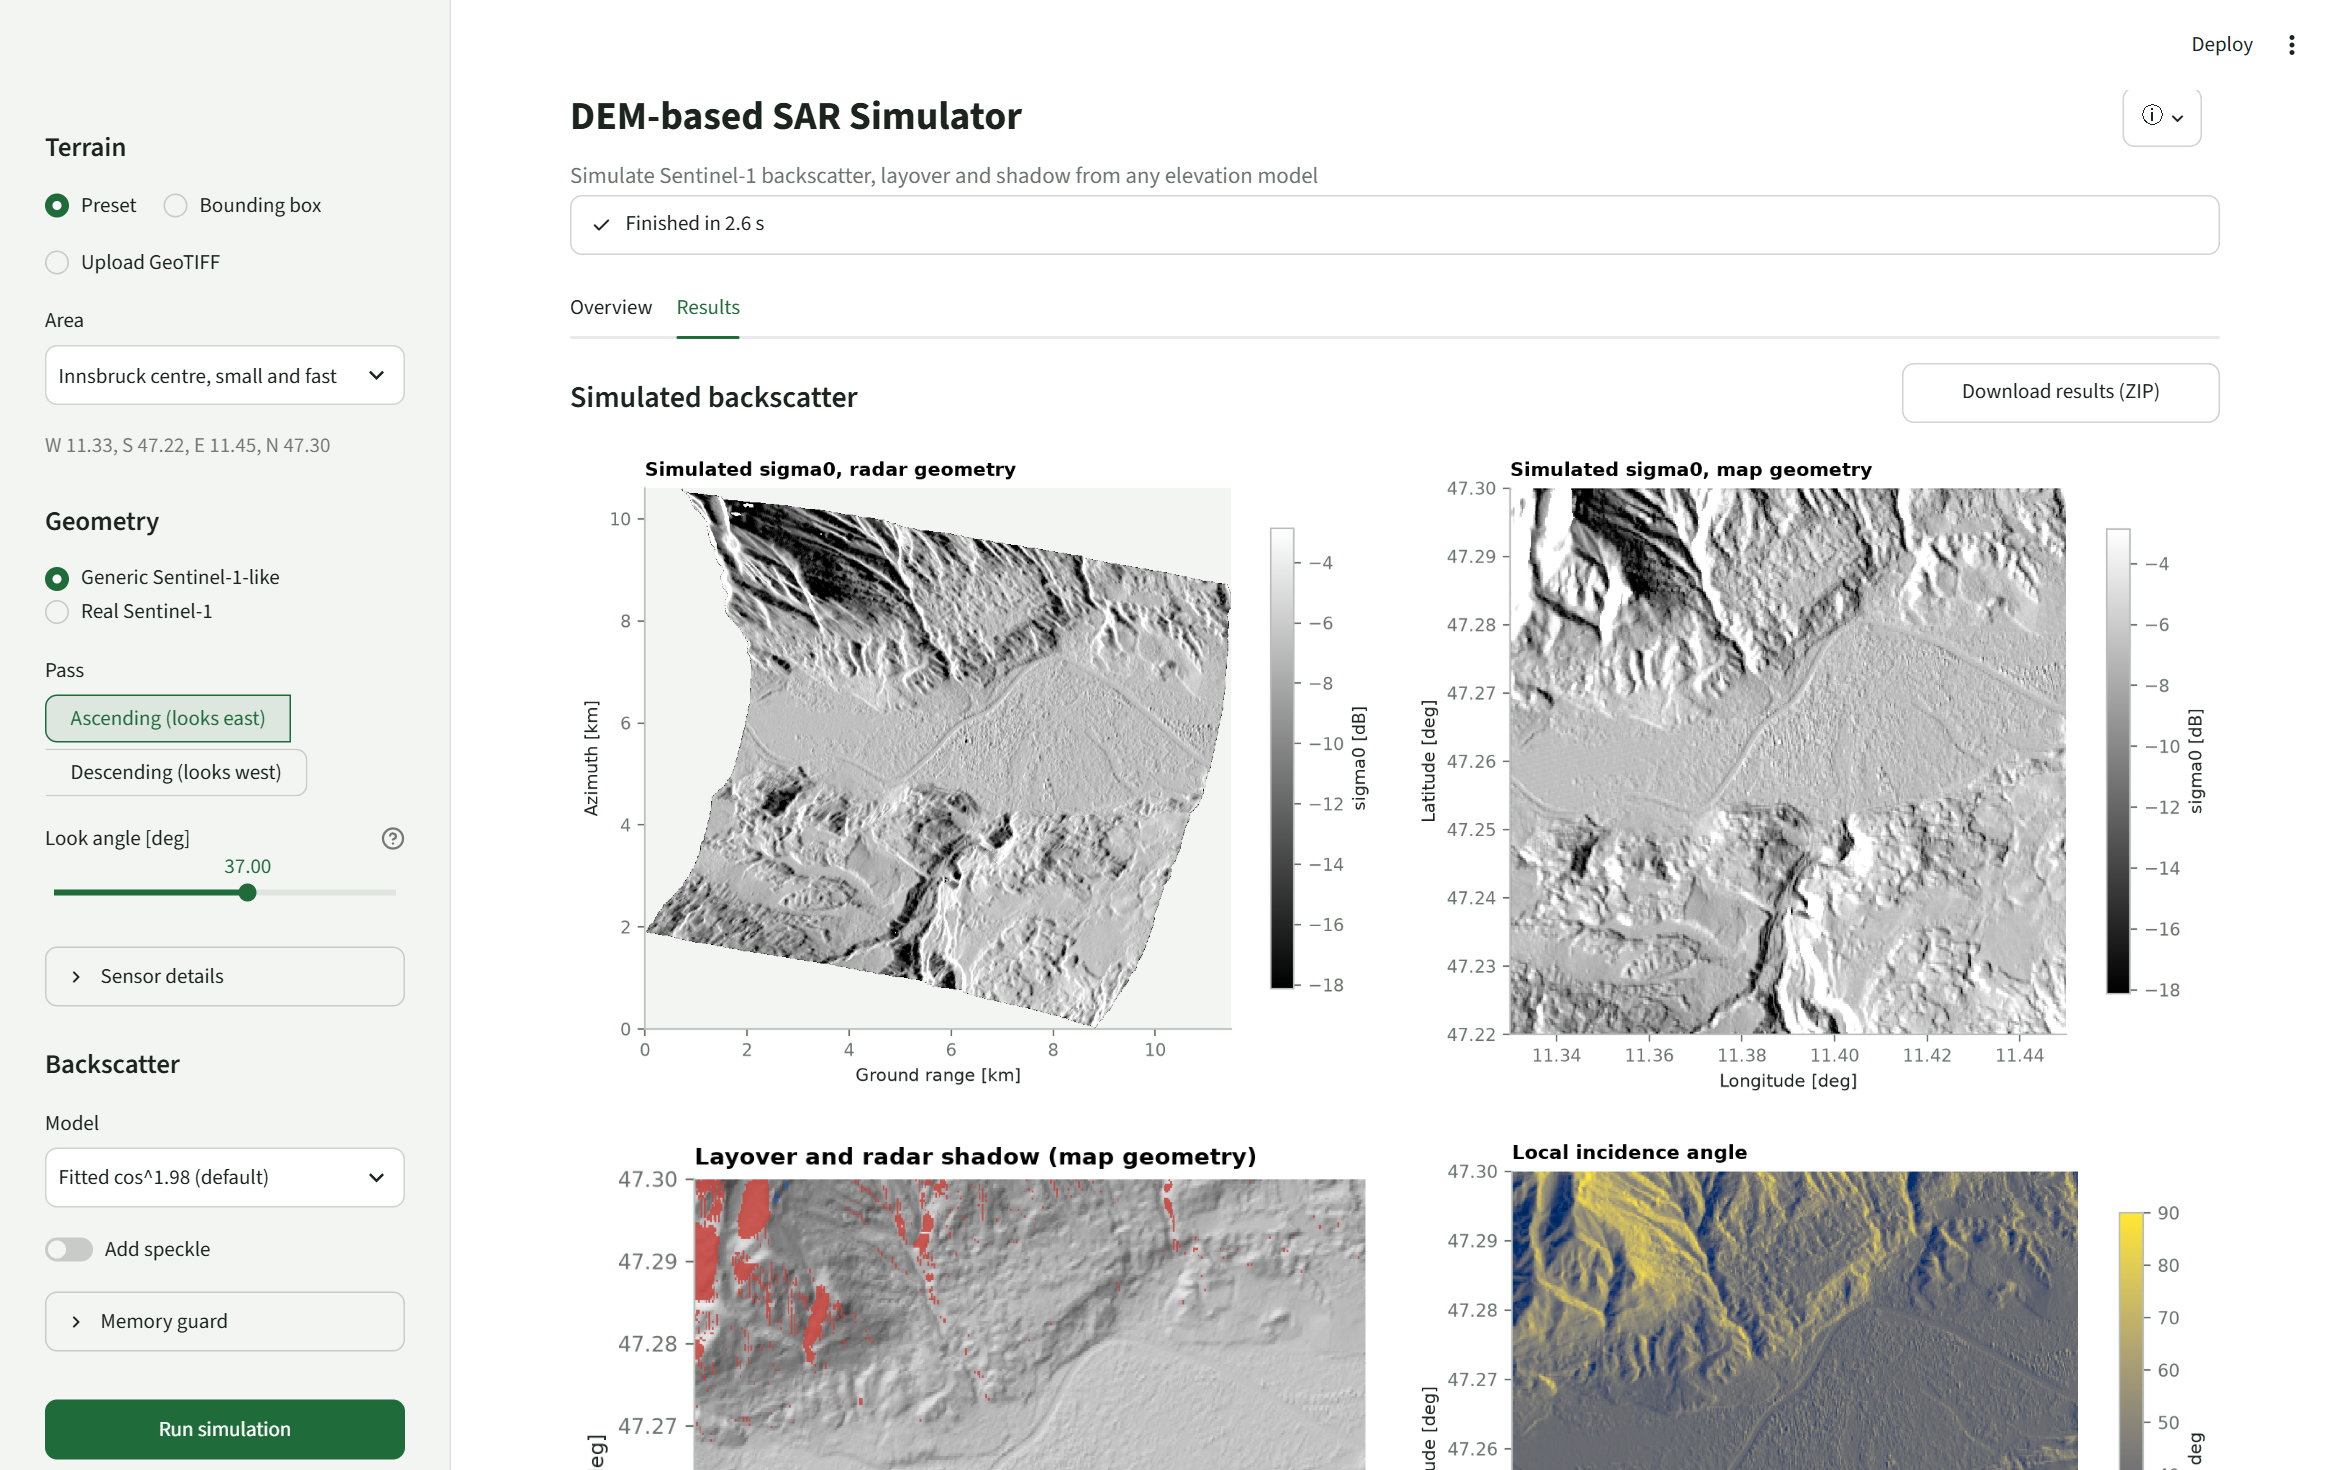
\includegraphics[width=\textwidth]{gui_04_results.png}
\caption[Graphical application: Results tab]{Graphical application: Results tab with the download button, the simulated
$\sigma^0$ in radar and map geometry, the layover and shadow masks and the local incidence angle.}
\label{fig:gui-results}
\end{figure}

\chapter{Conclusions and Scope for Future Work}
\label{ch:conclusions}

\section{Conclusions}
This study developed a SAR simulator from first principles and assessed how far a simulation driven only by a DEM and
the annotated orbit of the product predicts real Sentinel-1 images of Alpine terrain. A raw-signal simulator, verified
against theory from the impulse response of a point target to a real DEM, validated a fast image-domain simulator
($r=0.97$). Range-Doppler geocoding with the annotated orbit reproduced the geolocation grid of the products to
\geoDpixMax{} pixels, provided that the slant-to-ground-range polynomials are applied piece-wise rather than
interpolated; interpolation caused errors of up to 3.3 pixels. Predicted shadow and layover coincided with the darkest
and brightest real pixels in both viewing geometries. A local-incidence-angle law $k\cos^{n}\theta_{loc}$ fitted to
the ascending scene, with $n=\nFit$ (close to Lambert's law), reproduced the real $\sigma^0$ with $r=\rAsc$ and
transferred unchanged to the descending scene ($r=\rDesc$). Geoid correction and DEM oversampling proved essential for
products at full resolution, while a 90\,m DEM sufficed at the 50\,m scale of the comparison. The remaining
disagreement is dominated by land cover: forest was reproduced without bias, whereas built-up areas and bare rock were
about 3\,dB brighter and water about 4\,dB darker than predicted.

\section{Scope for Future Work}
Several extensions follow directly from the limitations of this study. First, land-cover-dependent backscatter laws,
for example one law per WorldCover class, would address the largest part of the remaining radiometric disagreement.
Second, a double-bounce term for built-up areas, derived from building footprints and heights, would explain the
residuals over the city. Third, thermal-noise removal would allow predicted shadow to be compared with zero rather than
with the noise floor. Fourth, multi-temporal stacks of Sentinel-1 images would separate seasonal effects such as snow
cover and soil moisture from the terrain signal. Finally, the simulated illuminated-area image and the layover and
shadow masks can be used directly for radiometric terrain flattening and for automatic simulation-based
co-registration of Sentinel-1 products.


% REFERENCES
\cleardoublepage
\bibliographystyle{unsrtnat}
\bibliography{references}

% APPENDICES
\appendix
\chapter{Code and Data Availability}
\label{app:code}
\noindent\begin{minipage}{0.66\textwidth}
The \texttt{sarsim} package, the experiment pipeline \texttt{run\_all.py}, the unit tests, the tutorial notebook, the
graphical application, this report and the posters are available at\\[4pt]
\url{\repoURL}\\[4pt]
All input data are downloaded from the Microsoft Planetary Computer without registration and cached locally.
\end{minipage}\hfill
\begin{minipage}{0.30\textwidth}\centering

\includegraphics[width=\textwidth]{qr_repo.png}\\[2pt]
{\small Repository}
\end{minipage}

\section*{Reproducing the Results}
The environment is pinned with \texttt{uv} (Python 3.12). Every number and figure of this report is reproduced by:
\begin{verbatim}
uv sync
uv run pytest -q tests
uv run python run_all.py
uv run python report/make_tables.py
\end{verbatim}

\section*{Sentinel-1 Products}
{\scriptsize\ttfamily \sceneAsc\\ \sceneDesc\par}

\chapter{Simulation Parameters and Repository Structure}
\label{app:structure}

\section*{Parameters of the Raw-Signal Simulator}
\begin{table}[H]
\centering\small
\caption{Parameters of the Sentinel-1-like sensor used by the raw-signal simulator.}
\label{tab:sensor}
\resizebox{\textwidth}{!}{%
\begin{tabular}{lr@{\hspace{1.2cm}}lr}
\toprule
wavelength & 5.55\,cm & synthetic aperture $L_{sa}$ & 3.81\,km\\
orbit height & 693\,km & processed aperture & $\pm0.6\,L_{sa}$\\
look angle & 35$^\circ$ & slant / ground-range resolution & 3.00 / 5.23\,m\\
slant range (centre) & 846.0\,km & azimuth resolution $L/2$ & 6.15\,m\\
chirp bandwidth / length & 50\,MHz / 10\,$\mu$s & range sampling & 60\,MHz (2.50\,m)\\
PRF / pulse spacing & 1700\,Hz / 4.47\,m & antenna & $12.3\times0.821$\,m\\
\bottomrule
\end{tabular}}
\end{table}

\section*{Repository Structure}
{\small
\begin{tabularx}{\textwidth}{lX}\toprule
\texttt{sarsim/s1.py} & annotation parser, orbit fit, zero-Doppler geocoding, SRGR conversion, calibration\\
\texttt{sarsim/rdsim.py} & facet geometry, shadow and layover, backscatter laws, rendering\\
\texttt{sarsim/compare.py} & multilooking, co-registration, metrics, back-geocoding\\
\texttt{sarsim/data.py} & cached access to GLO-30, Sentinel-1 GRD windows and WorldCover\\
\texttt{sarsim/geodesy.py} & geodetic and ECEF conversions, EGM2008 geoid undulation\\
\texttt{run\_all.py} & experiments E1 to E5; figures in \texttt{figures/pipeline/}, results in \texttt{results/}\\
\texttt{notebooks/} & tutorial notebook (executed \texttt{.ipynb} and jupytext \texttt{.py} source)\\
\texttt{tests/} & unit tests\\
\texttt{report/} & article-style manuscript and this report (\texttt{report/btp/})\\
\texttt{poster/} & A3 academic poster, A1 newspaper-style poster and Canva package\\
\bottomrule\end{tabularx}\par}


\end{document}
